\documentclass[pfe ,titlesmallcaps]{isipfe}
\usepackage[T1]{fontenc}
\usepackage[utf8]{inputenc}
\graphicspath{{./Figures/}}

\usepackage{hyperref}
\hypersetup{hidelinks}

\usepackage{algorithm}
\usepackage{algorithmic}
\usepackage{float}
\usepackage{listings}
\usepackage{acronym}
\usepackage{textcomp}
% \usepackage[french]{babel}
\usepackage{enumitem}
\usepackage{longtable}
\setlength{\LTpre}{0pt}
\setlength{\LTpost}{0pt}
\usepackage{multirow}

\usepackage[table]{xcolor}
\usepackage{tcolorbox}
\usepackage{geometry}
\geometry{
  a4paper,
  left=25mm,
  right=25mm,
  top=25mm,
  bottom=25mm
}


\usepackage{array}
\definecolor{codebg}{HTML}{F7F9FC}
\definecolor{codetitle}{HTML}{1F4E79}
\definecolor{codekeyword}{HTML}{005A9E}
\definecolor{codestring}{HTML}{A31515}
\definecolor{codecomment}{HTML}{008000}
\definecolor{codeframe}{HTML}{D0D7DE}
\lstdefinelanguage{YAML}{
  sensitive=false,
  morecomment=[l]{\#},
  morestring=[b]",
  morestring=[b]'
}
\lstset{
  language=Java,
  basicstyle=\ttfamily\small,
  breaklines=true,
  columns=fullflexible,
  keepspaces=true,
  showstringspaces=false,
  frame=single,
  captionpos=b,
  rulecolor=\color{codeframe},
  backgroundcolor=\color{codebg},
  keywordstyle=\color{codekeyword}\bfseries,
  commentstyle=\color{codecomment}\itshape,
  stringstyle=\color{codestring},
  numbers=left,
  numberstyle=\tiny\color{black!55},
  numbersep=6pt,
  xleftmargin=1.8em,
  framexleftmargin=1.2em
}
\definecolor{niveauCritique}{HTML}{F8CBAD}
\definecolor{niveauEleve}{HTML}{B7DEE8}
\definecolor{niveauMoyen}{HTML}{FFF2CC}
\definecolor{niveauFaible}{HTML}{E2F0D9}

\usepackage{fontspec}
\usepackage{polyglossia}
\setmainlanguage{french}
\setotherlanguages{english,arabic}
\newfontfamily\arabicfont[Script=Arabic]{Arial}

\begin{document}

\frontmatter

\definecolor{isiBlue}{RGB}{79,129,189}

\newgeometry{bottom=20mm,left=20mm,top=15mm,right=20mm}

\begin{titlepage}
  \begin{center}

    %------------------------------------------------
    % Logos + Institution
    %------------------------------------------------

    \begin{center}
      \begin{minipage}{0.55\textwidth}
        \centering
        \footnotesize\textbf{
          RÉPUBLIQUE TUNISIENNE\\
          Ministère de l'Enseignement Supérieur et de la Recherche Scientifique\\
          Établissement d'enseignement supérieur privé\\
          Ecole Supérieure Privée de Technologie et Ingénierie
        }
      \end{minipage}
    \end{center}

    \vspace{2cm}

    %------------------------------------------------
    % Report Type
    %------------------------------------------------

    {\Large\textbf{\textsc{RAPPORT DE PROJET DE DÉVELOPPEMENT}}}

    \vspace{1cm}

    {\small\textbf{Spécialité : Génie Logiciel et Systèmes d'Information}}

    \vspace{0.7cm}

    \textit{Réalisé par}

    \vspace{0.3cm}

    {\Large\textbf{Wassim Masmoudi}}\\
    {\Large\textbf{Souheil Moussa}}\\
    {\Large\textbf{Maila Kdous}}\\
    {\Large\textbf{Yasmine Riahi}}

    \vspace{0.6cm}

    %------------------------------------------------
    % Project Title
    %------------------------------------------------

    \begin{tcolorbox}[
        colframe=isiBlue,
        colback=white,
        boxrule=1.5pt,
        arc=3pt,
        width=0.95\textwidth,
        center title
      ]

      \centering
      {\large\bfseries PLANORA}

    \end{tcolorbox}

    \vspace{0.4cm}

    %------------------------------------------------
    % Supervisors
    %------------------------------------------------

    \textbf{Supervisé par:}\\
    Mme. Sonia Gharsalli \\
    Mr. Mohamed Alouani


      %------------------------------------------------
      % Company Logo
      %------------------------------------------------

      {\large\textbf{Réalisé au sein de TEKUP}}\\[0.6cm]
    
\includegraphics[width=0.5\textwidth]{tek_up_logo.jpg}

    \vfill

    %------------------------------------------------
    % Year
    %------------------------------------------------

    {\large Année Universitaire : 2025 / 2026}

  \end{center}
\end{titlepage}

\restoregeometry

\setcounter{secnumdepth}{3}
\setcounter{tocdepth}{2}
\tableofcontents

\listoffigures
\listoftables
\cleardoublepage
\markboth{}{}
\chapter*{Liste des abréviations}

\begingroup
\small
\begin{acronym}[PLANORA]
  \setlength{\itemsep}{0pt}
  \setlength{\parskip}{0pt}
  \acro{SSMS}{SQL Server Management Studio}
  \acro{VS}{Visual Studio}
  \acro{VSCode}{Visual Studio Code}
  \acro{API}{Application Programming Interface}
  \acro{JWT}{JSON Web Token}
  \acro{SQL}{Structured Query Language}
  \acro{JSON}{JavaScript Object Notation}
  \acro{REST}{Representational State Transfer}
  \acro{ASPNET}{ASP.NET}
  \acro{DOTNET}{.NET}
  \acro{DTO}{Data Transfer Object}
  \acro{EF}{Entity Framework}
  \acro{SignalR}{SignalR}
  \acro{IA}{Intelligence Artificielle}
  \acro{UML}{Unified Modeling Language}
\end{acronym}
\endgroup

\mainmatter
\chapter*{}
\vspace{-3em}
{\raggedleft\huge\bfseries Introduction générale\par}
\vspace{2em}
\label{chap:intro}

De nos jours, la gestion de projet et la collaboration au sein des équipes constituent des enjeux essentiels pour les organisations. Face à la complexité croissante des projets, à la multiplication des tâches et à la nécessité d'assurer une bonne coordination entre les membres, l'utilisation d'outils numériques adaptés devient indispensable. Les équipes de développement logiciel, en particulier, ont besoin de solutions permettant de planifier les travaux, suivre l'avancement, gérer les priorités et favoriser une communication efficace.

Planora se présente comme une application web de gestion de projet conçue pour répondre aux besoins des équipes travaillant selon une approche collaborative et agile. Elle permet de centraliser les projets, les espaces de travail, les tâches, les backlogs, les sprints, les réunions et les échanges entre les membres. L'application intègre également des fonctionnalités intelligentes liées à l'analyse de la santé de l'équipe, afin d'aider les responsables à mieux comprendre l'état général du groupe et à détecter les signes de stress ou de frustration.

C'est dans ce cadre que s'inscrit ce projet de fin d'études, visant à concevoir et développer une plateforme complète de gestion de projet nommée Planora. Ce projet englobe la mise en place d'une architecture web basée sur un backend \ac{DOTNET}, un frontend Angular, ainsi qu'un module d'intelligence artificielle dédié à l'analyse des sentiments à partir des messages échangés entre les membres de l'équipe. L'objectif principal est de proposer une solution centralisée, ergonomique et évolutive permettant d'améliorer l'organisation, le suivi et la collaboration au sein des projets.

Le présent rapport est articulé autour des chapitres suivants :
\begin{itemize}
  \item Dans le premier chapitre, intitulé « Contexte général », nous présentons le cadre général du projet Planora, son domaine d'application, l'étude de l'existant ainsi que la méthodologie de gestion de projet retenue.
  \item Dans le deuxième chapitre, nommé « Analyse et spécification des besoins », nous identifions les acteurs du système et définissons les besoins fonctionnels et non fonctionnels. Nous y détaillons les principales fonctionnalités de l'application à travers des diagrammes de cas d'utilisation.
  \item Dans le troisième chapitre, « Conception », nous présentons l'architecture générale de la solution, la modélisation des données, les diagrammes de classes et les principaux scénarios d'interaction entre les différents composants du système.
  \item Dans le quatrième et dernier chapitre, intitulé « Réalisation », nous décrivons l'environnement de développement, les outils et technologies employés, ainsi que les interfaces les plus représentatives de l'application réalisée.
\end{itemize}

Ce rapport se clôturera par une conclusion synthétisant les acquis du projet et mettant en lumière les perspectives d'amélioration envisageables pour enrichir davantage les fonctionnalités de Planora.

%%%%% Chapter one
\chapter{Contexte général}

\section*{Introduction}
Ce chapitre introductif détaillera l'étude de l'existant, la problématique associée, ainsi qu'une évaluation approfondie de la solution proposée et des objectifs globaux du projet. Enfin, la dernière partie définira la méthodologie de gestion de projet adoptée.

\section{Présentation du cadre du projet}
Dans cette section, nous fournirons une analyse critique de l'existant, ainsi qu'une présentation détaillée de la solution proposée.
\subsection{Etude de l'existant}
Avant le développement de l'application Planora, une étude de l'existant a été réalisée afin d'analyser les solutions déjà disponibles sur le marché dans le domaine de la gestion de projets et du suivi collaboratif.Plusieurs plateformes et applications web proposent des fonctionnalités similaires, telles que la création de projets, la gestion des tâches, l'organisation des sprints, le suivi du backlog ou encore la collaboration entre les membres d'une équipe.\\
Parmi les solutions existantes, on retrouve des outils de gestion de projet comme Jira, Trello, Asana ou Monday.com, ainsi que des plateformes orientées vers les méthodes agiles et la communication d'équipe. Certaines de ces solutions intègrent également des tableaux de bord, des calendriers, des espaces de discussion, des systèmes de notification et des fonctionnalités d'analyse pour accompagner les équipes dans le suivi de leur avancement.\\
Cette étude a permis d'identifier les fonctionnalités communes, les bonnes pratiques ainsi que les limites techniques et fonctionnelles des solutions existantes, notamment en matière de centralisation des données, de suivi de la santé de l'équipe et d'intégration de fonctionnalités intelligentes d'aide à la décision.

\subsection{Tableau comparatif des solutions existantes}

Le tableau \ref{tab:comparaisonSolutions} présente une comparaison entre quelques solutions existantes de gestion de projet et la solution proposée Planora.

Dans ce tableau, la mention « Partiel » indique que la fonctionnalité existe de manière limitée ou nécessite une intégration avec un outil externe.

\begin{longtable}[c]{|p{0.14\textwidth}|p{0.22\textwidth}|p{0.20\textwidth}|p{0.20\textwidth}|p{0.18\textwidth}|}
  \caption{Comparaison entre les solutions existantes et Planora}
  \label{tab:comparaisonSolutions}                                                                                                                                                                                                                                                                                       \\

  \hline
  \textbf{Solution} & \textbf{Tâches, backlog et sprints}                                            & \textbf{Chat}                                       & \textbf{Réunions et calendrier}                              & \textbf{Analyse intelligente}                                                                \\
  \hline
  \endfirsthead

  \hline
  \textbf{Solution} & \textbf{Tâches, backlog et sprints}                                            & \textbf{Chat}                                       & \textbf{Réunions et calendrier}                              & \textbf{Analyse intelligente}                                                                \\
  \hline
  \endhead

  \hline
  \endlastfoot

  Jira              & Oui                                                                            & Partiel : via intégration avec Slack ou Teams       & Partiel : via intégration avec Google Calendar ou Outlook    & Non                                                                                          \\
  \hline
  Trello            & Partielle : gestion simple des cartes, sans sprints avancés natifs             & Partiel : via commentaires ou intégrations externes & Limitée : calendrier disponible selon les vues et extensions & Non                                                                                          \\
  \hline
  Asana             & Partielle : gestion des tâches avancée mais backlog et sprints non spécialisés & Partiel : via commentaires ou intégrations externes & Oui                                                          & Non                                                                                          \\
  \hline
  Monday.com        & Partielle : gestion personnalisable mais agile avancé selon configuration      & Oui                                                 & Oui                                                          & Non                                                                                          \\
  \hline
  Planora           & Oui                                                                            & Oui                                                 & Oui                                                          & Oui : analyse des messages pour détecter le stress, la frustration et l'ambiance de l'équipe \\
  \hline
\end{longtable}

\subsection{Critique de l'existant}
Malgré la diversité des solutions existantes, plusieurs insuffisances ont été constatées. La majorité des plateformes de gestion de projet proposent des fonctionnalités intéressantes, telles que la gestion des tâches, la planification des sprints ou le suivi de l'avancement, mais elles restent parfois dispersées entre plusieurs outils, ce qui complique le travail des équipes et limite la centralisation des informations.\\
De plus, certaines applications manquent de simplicité dans leur utilisation, notamment pour les équipes qui souhaitent adopter rapidement une méthode agile sans configuration complexe. L'absence d'un suivi précis de la santé de l'équipe constitue également une limite importante, car la plupart des solutions se concentrent principalement sur l'avancement technique du projet sans prendre en compte l'état général des membres, le stress ou la frustration exprimés pendant la collaboration.\\
Par ailleurs, les fonctionnalités de communication, de gestion des réunions et d'aide intelligente à la décision ne sont pas toujours intégrées dans une même plateforme, ce qui oblige les utilisateurs à utiliser plusieurs outils en parallèle. Ces limites soulignent la nécessité de concevoir une solution plus complète, centralisée et centrée sur les besoins réels des équipes de projet.

\subsection{Solution proposée}
Afin de remédier aux limites identifiées, le projet Planora propose une solution web complète regroupant plusieurs services de gestion de projet au sein d'une seule plateforme.\\
L'application permet aux utilisateurs de créer un compte sécurisé, de gérer des espaces de travail, de créer des projets, d'inviter des membres et d'organiser les tâches selon une approche collaborative et agile. Elle offre également la possibilité de gérer le backlog, les sprints, les sous-tâches, les réunions ainsi que le suivi de l'avancement à travers des tableaux de bord.\\
L'intégration d'un module basé sur l'intelligence artificielle constitue un élément différenciateur majeur, permettant d'analyser les messages échangés entre les membres afin d'évaluer la santé de l'équipe et de détecter les signes de stress ou de frustration. De plus, la plateforme intègre un espace de messagerie favorisant la communication et la coordination entre les membres du projet.\\
Cette solution vise à améliorer l'organisation, la collaboration et le suivi des projets tout en assurant une expérience utilisateur cohérente, centralisée et adaptée aux besoins réels des équipes.

\section{Choix Méthodologique}
Il est primordial d'opter pour la bonne méthodologie avant de débuter un projet informatique. En effet, aucune méthode universelle ne peut garantir à elle seule
l'exécution adéquate de l'ensemble des tâches d'un projet, tant les contextes et les objectifs varient d'un projet à l'autre.\\
La méthode sélectionnée doit donc être adaptée aux spécificités et aux contraintes de chaque projet. Ainsi, il est essentiel de retenir une approche qui réponde aux
besoins réels des parties prenantes, afin de garantir un résultat optimal et conforme aux attentes.\\
Dans le présent contexte, nous avons opté pour une approche de gestion de projet hybride, connue sous le nom de modèle \textbf{Water-Scrum-Fall}, qui combine les avantages des deux méthodologies les plus répandues :
\begin{itemize}
  \item La planification rigoureuse et la documentation exhaustive du \textbf{modèle
          en cascade} lors des phases d'audit et de conception, en s'appuyant sur \ac{UML}
        comme langage de modélisation.
  \item Le développement itératif et incrémental de la méthodologie \textbf{Scrum}
        lors des phases de mise en place et de développement, organisé en sprints permettant des livraisons régulières et une adaptation continue aux retours obtenus.
\end{itemize}

La figure \ref{MethHybride} ci-dessous illustre la méthodologie hybride adoptée :
\begin{figure}[H]
  \centering
  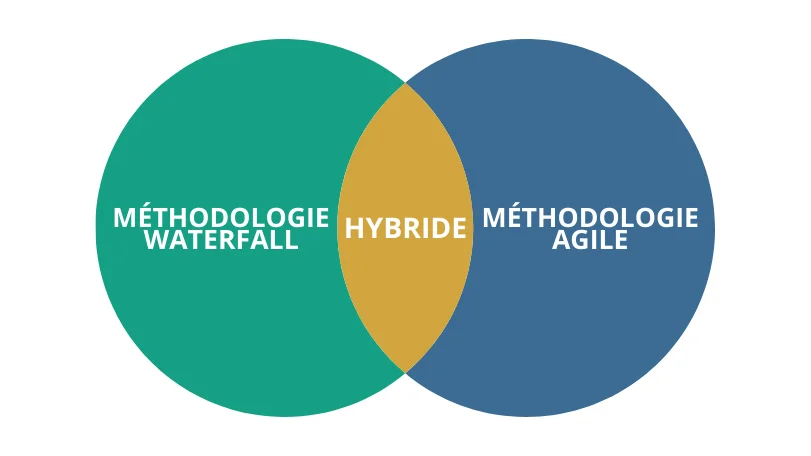
\includegraphics[width=0.6\columnwidth]{MethHybride.png}
  \caption{Méthodologie Hybride adoptée\cite{HybridMeth}}
  \label{MethHybride}
\end{figure}

En tirant parti des forces de chaque méthodologie, cette approche hybride vise à maximiser l'efficacité, à atténuer les risques et à assurer une livraison progressive et contrôlée des différents composants du projet.

\subsection{Méthodologie du modèle en cascade}
Le modèle en cascade, caractérisé par son approche séquentielle, est souvent associé lors de la phase de conception dans nombreux projets. Cette approche garantit une analyse approfondie des exigences et des objectifs du projet, suivie par la conception d'une solution complète et détaillée répondant à ces exigences. \\
Cette conception est ensuite examinée et validée avant de passer à la phase de développement proprement dite.\\
La linéarité du processus en cascade permet une gestion efficace des ressources et une planification minutieuse des étapes, offrant une structure et une prévisibilité précieuses dans la phase d'analyse des besoins et de conception\cite{Waterfall}
\subsection{Méthodologie agile}
La méthodologie Agile adoptée durant le cycle de vie de développement se distingue
des approches traditionnelles telles que le cycle en V ou le modèle en cascade, qui nécessitent une planification complète du projet avant le début du développement, par sa flexibilité et son adaptabilité en se concentrent sur des objectifs à court terme. \\
Plaçant le client au cœur du processus, cette approche favorise une collaboration étroite et des retours réguliers, ce qui permet à l'équipe de développement d'intégrer rapidement les modifications nécessaires pour répondre aux évolutions du projet\cite{MethAgile}.
La figure \ref{CycleDevAgile} ci-dessous illustre le cycle de vie de développement d'un logiciel agile :
\begin{figure}[H]
  \centering
  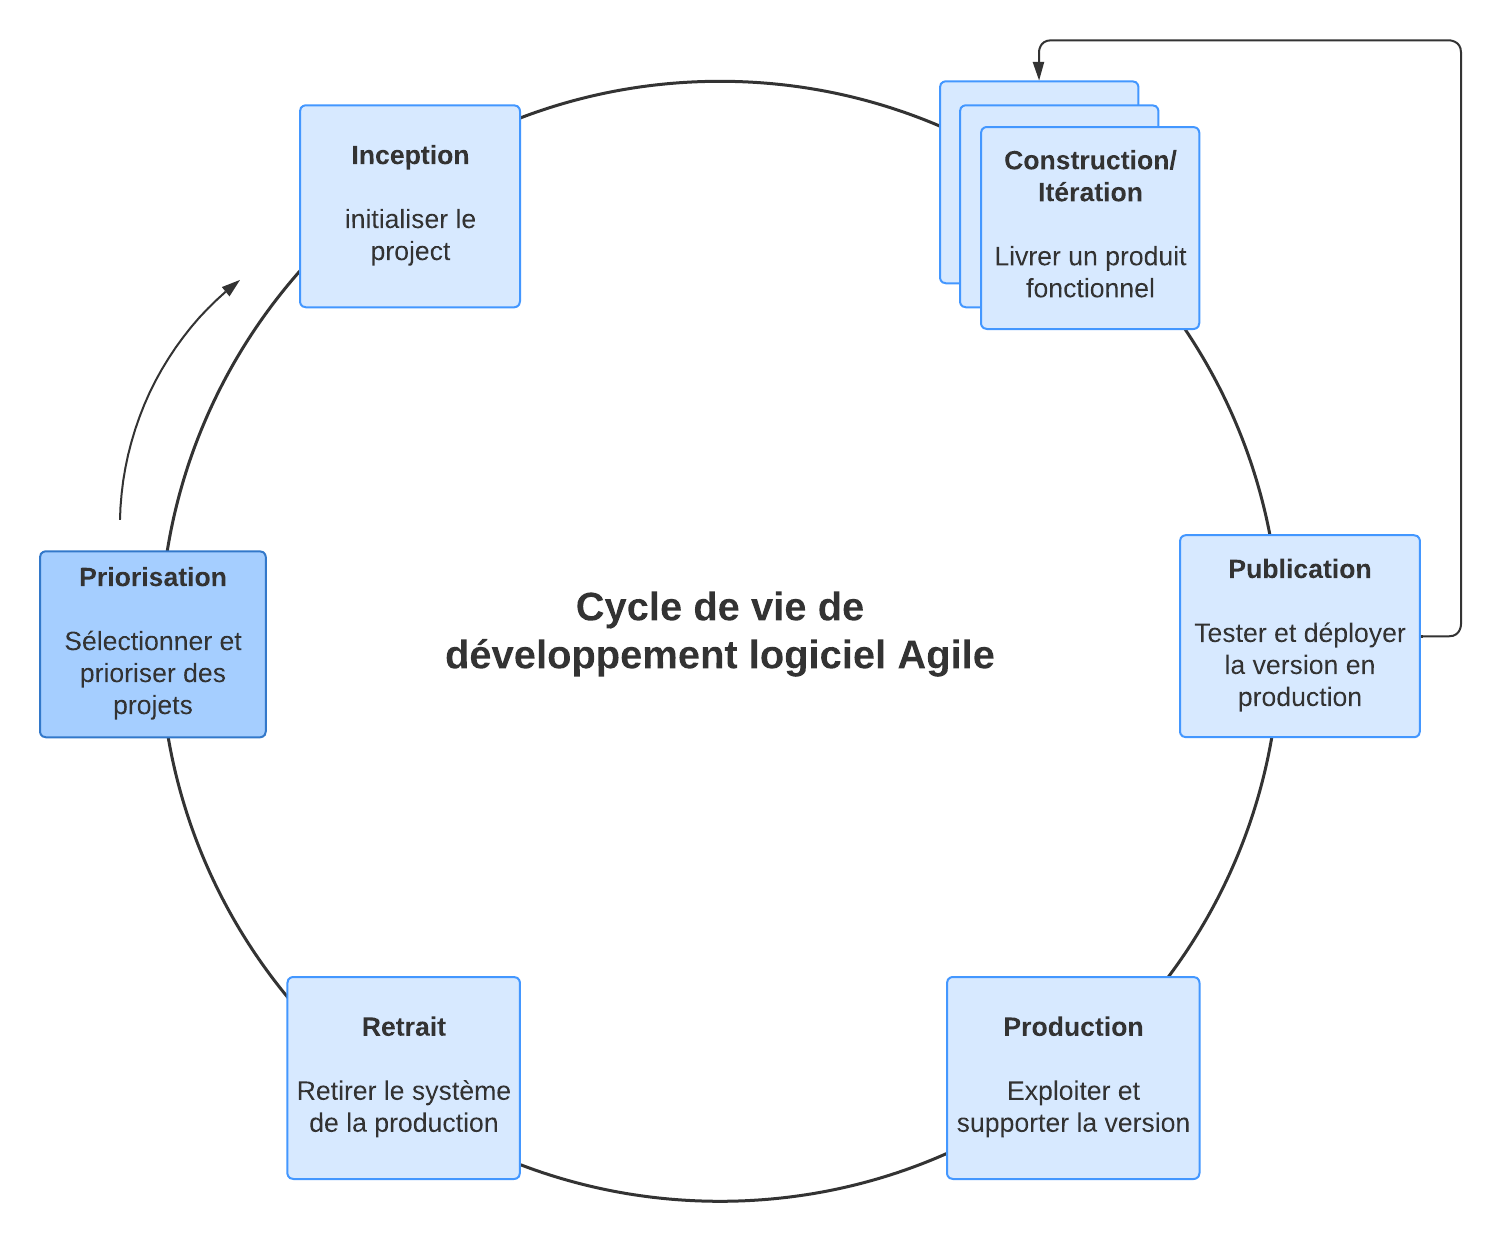
\includegraphics[width=0.85\columnwidth]{Agile Software Development Life Cycle.png}
  \caption{Cycle de vie de développement d'un logiciel agile}
  \label{CycleDevAgile}
\end{figure}
\subsubsection{Méthodologie Scrum}
La méthodologie Scrum est de loin la méthode Agile la plus utilisée dans le monde, offrant un cadre organisé pour superviser la création d'applications complexes. Cette approche intègre de différentes pratiques centralisées sur la flexibilité et la collaboration avec le client afin de s'adapter aux exigences changeantes tout en reposant sur la maintenance d'un « Backlog », qui décrit les changements ou améliorations à apporter sous forme des « user stories ».
\subsubsection{Caractéristiques de Scrum}
Les livraisons fréquentes sont une caractéristique clé de Scrum. Pour atteindre cet objectif, Scrum emploie des itérations de développement, connues sous le nom de « sprints », qui durent généralement de 2 à 4 semaines. Durant ces sprints, les opérations de développement traite activement les problématiques métier en cours, abordant les dossiers d'analyse et de conception afin de réaliser les phases de développement, de test et de déploiement\cite{ScrumCarac}.
\subsubsection{Rôles dans Scrum}
La méthodologie Scrum repose sur trois rôles essentiels :
\begin{itemize}
  \item Product Owner : chargé de déterminer et de donner la priorité aux éléments du backlog du produit. Celle-ci informe l'équipe de développement des besoins et des exigences du client et prend les décisions concernant les fonctionnalités à fournir.
  \item Scrum Master : garantir que l'équipe comprend et suit les principes et les méthodes de Scrum. Celui-ci facilite la communication des membres de l'équipe et soutient l'équipe dans l'accomplissement de ses objectifs.
  \item Équipe de développement : sont chargés de transférer les éléments du backlog produit en fonctionnalités livrables, celles-ci collaborent pour atteindre les objectifs du sprint et sont autonomes dans leur approche de travail.
\end{itemize}
La figure \ref{ProcScrum} ci-dessous illustre le processus de la méthode Scrum :
\begin{figure}[H]
  \centering
  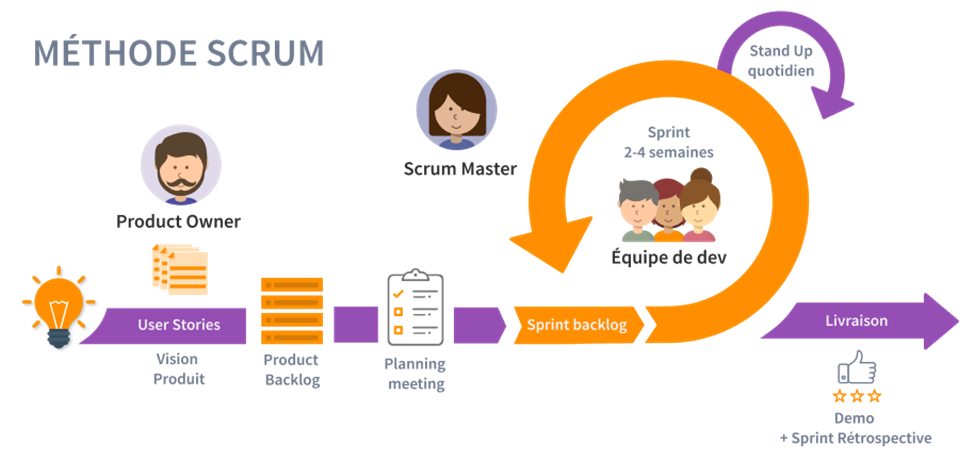
\includegraphics[width=1\columnwidth]{ProcScrum.png}
  \caption{Processus de la méthode Scrum}
  \label{ProcScrum}
\end{figure}
\section{Langage de Modélisation}
Le choix du langage de modélisation dans le présent projet a été porté sur \ac{UML}. Il est justifié par sa standardisation, sa capacité à clarifier et à documenter les spécifications du système, ainsi que par son utilité dans l'analyse, la conception, la maintenance et la validation du système logiciel.\\
En effet, \ac{UML} offre un ensemble de conventions visuelles pour représenter les systèmes et les processus à l'aide de diagrammes et de représentations graphiques. Cette approche simplifie la communication des concepts complexes, favorisant ainsi une collaboration fluide et une compréhension approfondie à chaque étape du développement et de la conception.
\subsection{Présentation de UML}
Le langage de modélisation \ac{UML} est l'un des langages de modélisation les plus couramment employés dans le domaine de l'ingénierie logicielle. \ac{UML} propose une méthode efficace pour représenter visuellement la structure, le comportement et les interactions d'un système logiciel en utilisant des diagrammes standardisés tels que les diagrammes de classes, de cas d'utilisation, de séquence et bien d'autres\cite{UML}.
\subsection{Diagrammes UML}
Le langage de modélisation \ac{UML} est défini par 14 types de diagrammes, distingués en deux catégories : "structure" et "comportement", afin de garantir une modélisation appropriée des caractéristiques de tout système.
Afin de garantir une modélisation complète et précise des fonctionnalités de la future application, nous avons choisi d'utiliser les diagrammes UML répertoriés dans le tableau \ref{tab:diagUmlTab} ci-dessous :

\begin{longtable}[c]{|p{0.25\textwidth}|p{0.65\textwidth}|}
  \caption{Types des diagrammes UML}
  \label{tab:diagUmlTab}                                                                                                                                                                                                                                                                                                                                                                                                                               \\

  \hline
  \textbf{Diagramme}             & \textbf{Description}                                                                                                                                                                                                                                                                                                                                                                                                \\
  \hline
  \endfirsthead
  \hline
  \textbf{Diagramme}             & \textbf{Description}                                                                                                                                                                                                                                                                                                                                                                                                \\
  \hline
  \endhead
  \hline
  \endlastfoot
  Diagramme de classe            & Le diagramme UML le plus largement utilisé, essentiel à toute approche orientée objet, est le diagramme de classe. Ce diagramme représente des entités spécifiques du système applicatif sous forme de classes. Chaque classe est composée d'attributs, définissant les caractéristiques des objets créés à partir de ces classes, ainsi que de méthodes, définissant les actions que ces objets peuvent effectuer. \\
  \hline
  Diagramme de cas d'utilisation & Le diagramme de cas d'utilisation représente une fonctionnalité spécifique dans un système applicatif et met en évidence les liens et les interactions avec ses différentes fonctionnalités à l'aide d'acteurs internes et externes.                                                                                                                                                                                \\
  \hline
  Diagramme de séquence          &
  Le diagramme de séquence illustre comment les objets d'un scénario spécifique interagissent les uns avec les autres dans un ordre chronologique.                                                                                                                                                                                                                                                                                                     \\
  \hline
\end{longtable}

\section*{Conclusion}
Dans ce premier chapitre, nous avons présenté le contexte général du projet Planora, en mettant en lumière l'étude de l'existant, la critique des solutions disponibles ainsi que la solution proposée. Nous avons également exposé le choix méthodologique adopté, basé sur une approche hybride Water-Scrum-Fall, ainsi que le langage de modélisation UML retenu pour la conception du système. Dans le chapitre suivant, nous approfondirons l'analyse et la spécification des besoins fonctionnels et non fonctionnels de l'application.

%%%%% Chapter two
\chapter{Analyse et Spécification des besoins}

\section*{Introduction}
Dans ce chapitre, nous identifierons les acteurs du projet et définirons les besoins fonctionnels et non fonctionnels. Ensuite, nous détaillerons toutes les fonctionnalités du projet à l'aide d'un diagramme de cas d'utilisation global et de ses raffinements. Enfin, nous présenterons le planning sous la forme d'un diagramme de Gantt et décrirons l'approche Scrum adoptée pour la gestion du projet.

\section{Spécification des besoins}
Dans cette section, nous présenterons les différents acteurs de l'application, ainsi que les besoins fonctionnels et non fonctionnels identifiés pour le projet.

\subsection{Identification des acteurs}
L'acteur, qu'il soit interne ou externe, physique ou logiciel, est une entité capable d'interagir directement avec le système applicatif. Dans ce cadre, nous avons identifié quatre acteurs, comme présenté dans le tableau \ref{tab:acteurIdent} ci-dessous :

\begin{longtable}[c]{|p{0.3\linewidth}|p{0.65\linewidth}|}
  \hline
  \textbf{Acteurs}            & \textbf{Description}                                                                                                                                                                                                                                                                                           \\
  \hline
  \endfirsthead

  \hline
  \textbf{Acteurs}            & \textbf{Description}                                                                                                                                                                                                                                                                                           \\
  \hline
  \endhead

  \hline
  \endfoot

  \hline
  \endlastfoot

  Administrateur              & Dispose d'un accès aux fonctionnalités d'administration de la plateforme. Il peut gérer les utilisateurs, attribuer les rôles, activer ou désactiver les comptes, créer et supprimer des espaces de travail, inviter des membres et supprimer des projets.                                                     \\
  \hline

  Chef de projet              & Responsable de la gestion des projets et de la collaboration au sein des espaces de travail auxquels il appartient. Il peut consulter les espaces accessibles, créer et modifier des projets, inviter des membres, gérer les tâches, le backlog, les sprints, les réunions et suivre l'avancement du projet.   \\
  \hline

  Membre                      & Représente un utilisateur appartenant à un espace de travail ou à un projet. Il peut consulter les projets auxquels il est affecté, participer aux discussions, consulter et mettre à jour les tâches, commenter les éléments du backlog, suivre les sprints et accéder aux réunions selon ses droits d'accès. \\
  \hline

  Utilisateur non authentifié & Peut accéder aux interfaces d'inscription et de connexion afin de créer un compte ou de s'authentifier pour accéder aux fonctionnalités de l'application.                                                                                                                                                      \\
  \hline

  \caption{\centering Identification des Acteurs et leurs Fonctions dans le Système Applicatif}
  \label{tab:acteurIdent}
\end{longtable}

\underline{\textbf{Remarque}}: Les fonctionnalités accessibles dépendent du rôle de l'utilisateur ainsi que de son appartenance à un espace de travail ou à un projet.

\subsection{Besoins fonctionnels}

La mise en \oe{}uvre de la future application Planora doit répondre aux besoins fonctionnels suivants :
\begin{itemize}
  \item[$\bullet$] \textbf{Gestion d'inscription :}
        \begin{itemize}
          \item[$\circ$] Création d'un nouveau compte utilisateur.
          \item[$\circ$] Enregistrement des informations personnelles de l'utilisateur.
        \end{itemize}

  \item[$\bullet$] \textbf{Gestion de l'authentification :}
        \begin{itemize}
          \item[$\circ$] Connexion sécurisée à l'application.
          \item[$\circ$] Gestion de la session utilisateur.
        \end{itemize}

  \item[$\bullet$] \textbf{Gestion des utilisateurs et de leurs droits d'accès :}
        \begin{itemize}
          \item[$\circ$] Consultation de la liste des utilisateurs.
          \item[$\circ$] Attribution des rôles aux utilisateurs.
          \item[$\circ$] Activation et désactivation des comptes utilisateurs.
        \end{itemize}

  \item[$\bullet$] \textbf{Gestion des espaces de travail :}
        \begin{itemize}
          \item[$\circ$] Création et consultation des espaces de travail.
          \item[$\circ$] Invitation des membres à rejoindre un espace de travail.
          \item[$\circ$] Acceptation ou refus des invitations reçues.
          \item[$\circ$] Suppression des membres d'un espace de travail.
        \end{itemize}

  \item[$\bullet$] \textbf{Gestion des projets :}
        \begin{itemize}
          \item[$\circ$] Création, consultation, modification et suppression des projets.
          \item[$\circ$] Ajout et suppression des membres d'un projet.
          \item[$\circ$] Invitation des membres à rejoindre un projet.
        \end{itemize}

  \item[$\bullet$] \textbf{Gestion du backlog :}
        \begin{itemize}
          \item[$\circ$] Création, modification et suppression des éléments du backlog.
          \item[$\circ$] Affectation des éléments du backlog aux membres.
          \item[$\circ$] Définition de la priorité, de la complexité, des story points et de la date d'échéance.
          \item[$\circ$] Ajout de commentaires, de liens, de branches, de commits et de pièces jointes.
        \end{itemize}

  \item[$\bullet$] \textbf{Gestion des tâches et sous-tâches :}
        \begin{itemize}
          \item[$\circ$] Création, consultation, modification et suppression des tâches.
          \item[$\circ$] Affectation des tâches aux membres du projet.
          \item[$\circ$] Suivi de l'état d'avancement des tâches et des sous-tâches.
        \end{itemize}

  \item[$\bullet$] \textbf{Gestion des sprints :}
        \begin{itemize}
          \item[$\circ$] Création, consultation, modification et suppression des sprints.
          \item[$\circ$] Association des éléments du backlog à un sprint.
          \item[$\circ$] Suivi de l'avancement des sprints à travers un tableau de bord agile.
        \end{itemize}

  \item[$\bullet$] \textbf{Gestion de la collaboration :}
        \begin{itemize}
          \item[$\circ$] Échange de messages entre les membres d'un projet.
          \item[$\circ$] Consultation des conversations liées aux projets.
          \item[$\circ$] Épinglage des messages importants.
        \end{itemize}

  \item[$\bullet$] \textbf{Gestion des réunions :}
        \begin{itemize}
          \item[$\circ$] Création et consultation des réunions.
          \item[$\circ$] Planification des réunions dans un calendrier.
          \item[$\circ$] Définition des membres concernés par chaque réunion.
        \end{itemize}

  \item[$\bullet$] \textbf{Suivi et analyse de la santé de l'équipe :}
        \begin{itemize}
          \item[$\circ$] Analyse des messages échangés entre les membres.
          \item[$\circ$] Détection du stress, de la frustration et de l'ambiance générale.
          \item[$\circ$] Génération d'indicateurs et d'alertes liés à la santé de l'équipe.
        \end{itemize}

  \item[$\bullet$] \textbf{Consultation du tableau de bord :}
        \begin{itemize}
          \item[$\circ$] Visualisation de l'avancement des projets.
          \item[$\circ$] Consultation des statistiques globales et des indicateurs de suivi.
        \end{itemize}
\end{itemize}

\subsection{Besoins non fonctionnels}
Les besoins non fonctionnels sont tout aussi cruciaux que les besoins fonctionnels dans tout projet, affectant la qualité, la sécurité et l'expérience utilisateur globale. Ils sont essentiels pour garantir la performance et la satisfaction des utilisateurs finaux.

\begin{itemize}[label=\textbullet]
  \item \textbf{Ergonomie :} L'application doit disposer d'une interface ergonomique, intuitive et conforme aux bonnes pratiques UI/UX, afin d'offrir une expérience utilisateur optimale.

  \item \textbf{Fiabilité :} L'application doit garantir une disponibilité élevée, des temps de réponse réduits et une gestion efficace des erreurs.

  \item \textbf{Maintenabilité :} Le code doit être organisé de manière claire, modulaire et documentée, afin de faciliter sa compréhension, son évolution et sa maintenance par d'autres développeurs.

  \item \textbf{Sécurité :} L'application doit intégrer un dispositif de sécurité cohérent garantissant l'intégrité, la disponibilité et la confidentialité des données, ainsi que l'authentification des utilisateurs.
\end{itemize}

\section {Diagramme de cas d'utilisation global}
Le diagramme de cas d'utilisation global présenté dans la figure \ref{fig:Use Case} offre une vue d'ensemble des interactions des acteurs avec les diverses fonctionnalités de l'application cible, permettant ainsi une compréhension rapide des fonctionnalités et des besoins des utilisateurs.

\begin{figure}[H]
  \centering
  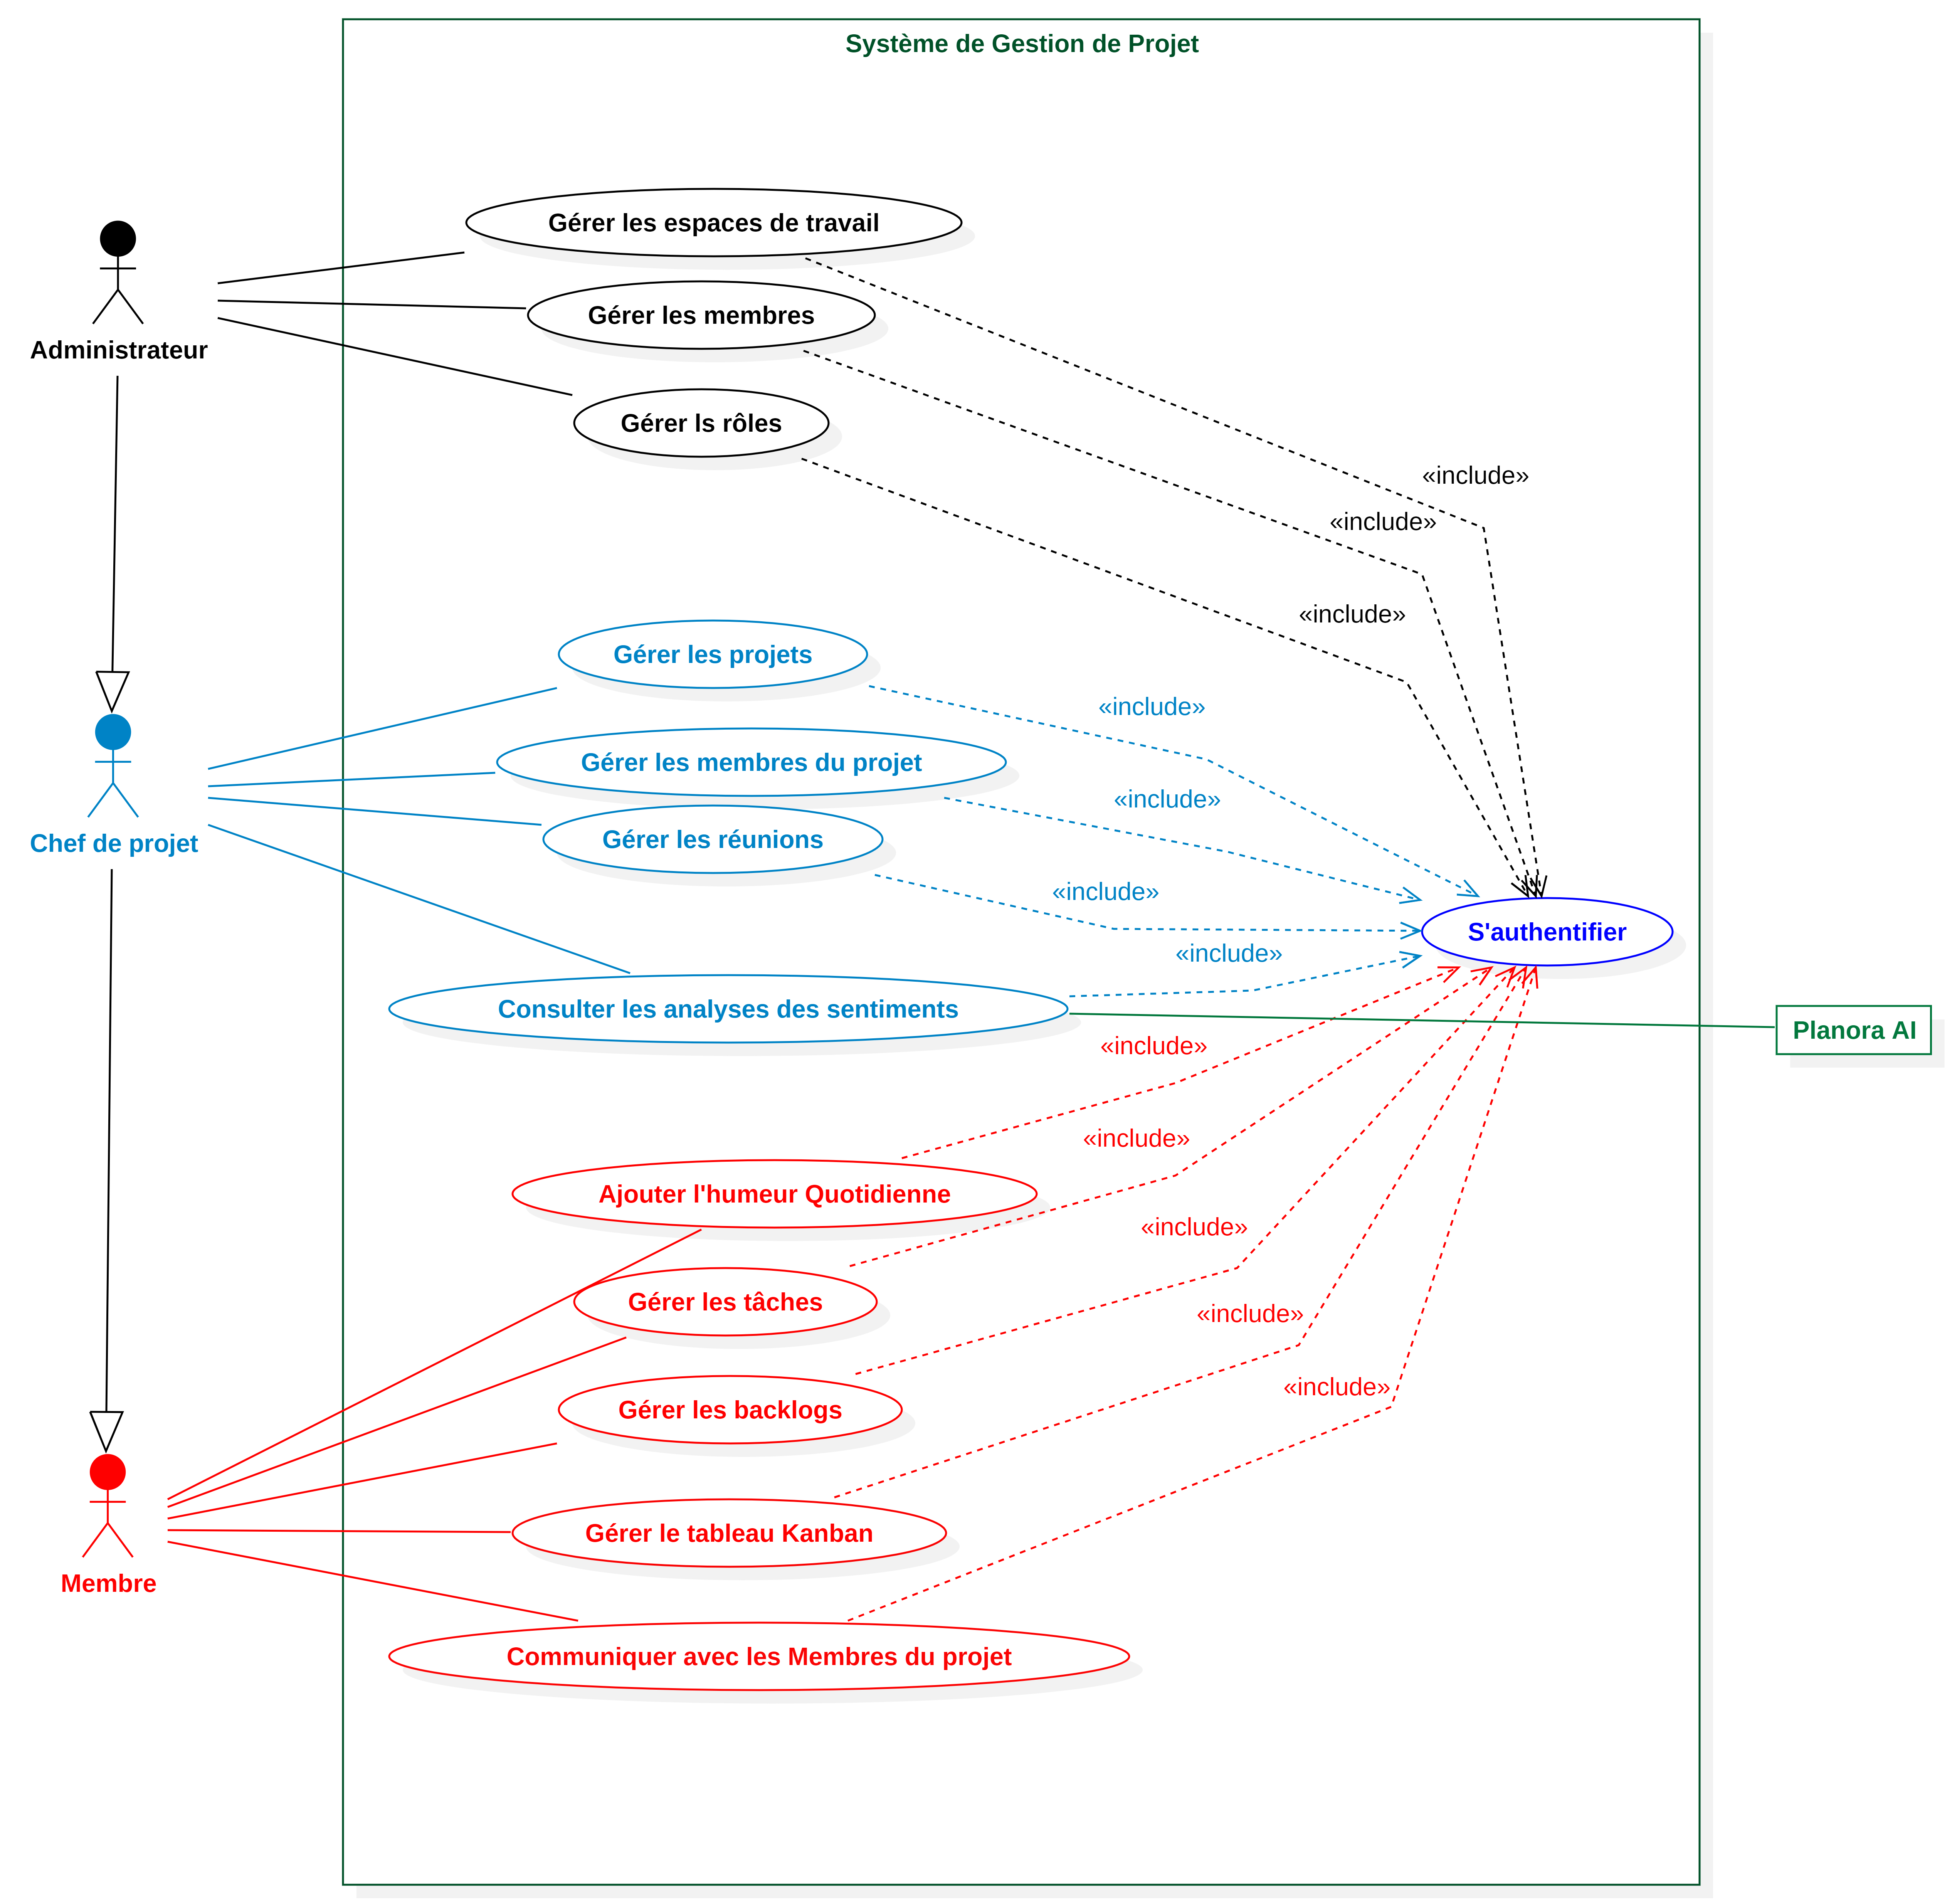
\includegraphics[width=1\linewidth]{UseCaseDiagram1.png}
  \caption{Diagramme de cas d'utilisation globale}
  \label{fig:Use Case}
\end{figure}

\section{Raffinement des cas d'utilisation}
\subsection{Gestion des membres et authentification}

 %La figure \ref{fig:GestionUtilisateurUseCase} ci-dessous illustre le diagramme de raffinement de la gestion des membres et de l'authentification.

 %\begin{figure}[H]
  % \centering
   % 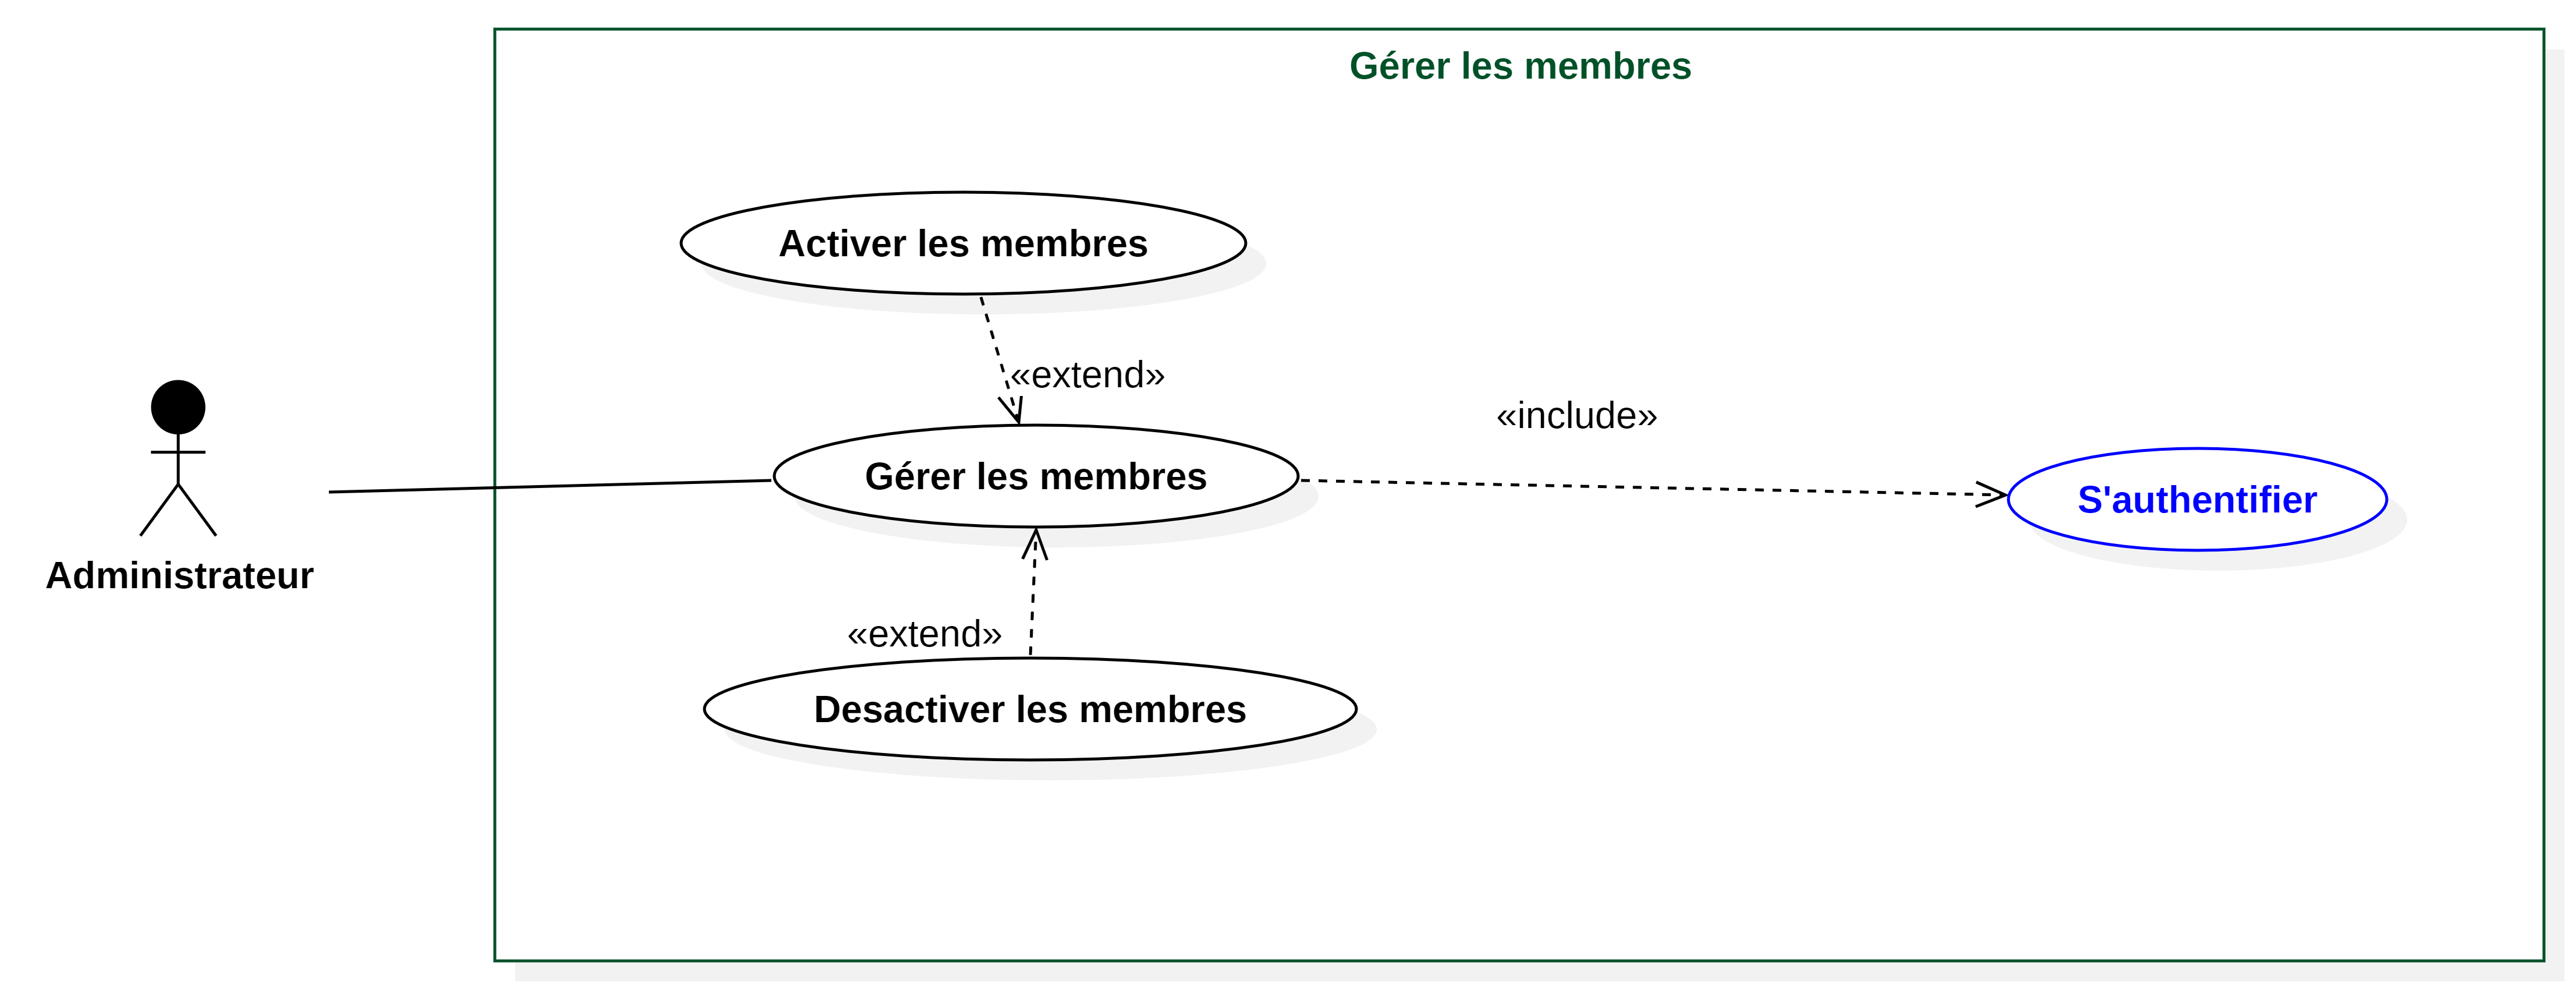
\includegraphics[width=1\columnwidth]{gererM.png}
   %\caption{Diagramme de cas d'utilisation « Gestion des utilisateurs et authentification »}
   % %\label{fig:GestionUtilisateurUseCase}
 %\end{figure}

Les tableaux ci-dessous présentent une description textuelle des cas d'utilisation liés à la gestion des utilisateurs.

\subsubsection{Utilisateur}

\begin{longtable}[c]{|p{0.3\linewidth}|p{0.65\linewidth}|}
  \hline
  \multicolumn{2}{|c|}{\textbf{S'authentifier}}                                                                                                  \\
  \hline
  \endfirsthead

  \hline
  \multicolumn{2}{|c|}{\textbf{S'authentifier}}                                                                                                  \\
  \hline
  \endhead

  \hline
  \endfoot

  \hline
  \endlastfoot

  \textbf{Objectif}      & Permettre à l'utilisateur d'accéder à l'application Planora selon son rôle.                                           \\
  \hline
  \textbf{Acteur(s)}     & Administrateur, ProjectManager, Membre                                                                                \\
  \hline
  \textbf{Précondition}  & L'utilisateur doit posséder un compte valide.                                                                         \\
  \hline
  \textbf{Scénario}      &
  1. L'utilisateur accède à la page de connexion.                                                                                                \\
                         & 2. L'utilisateur saisit son adresse email et son mot de passe.                                                        \\
                         & 3. Le système vérifie les informations d'identification.                                                              \\
                         & 4. Si les informations sont valides, le système génère une session et redirige l'utilisateur vers le tableau de bord. \\
                         & 5. Si les informations sont incorrectes, le système affiche un message d'erreur.                                      \\
  \hline
  \textbf{Postcondition} & L'utilisateur est authentifié et accède aux fonctionnalités autorisées selon son rôle.                                \\
  \hline
  \caption{\centering Description textuelle du cas d'utilisation « S'authentifier »}
\end{longtable}

\subsubsection{Administrateur}

\begin{longtable}[c]{|p{0.3\linewidth}|p{0.65\linewidth}|}
  \hline
  \multicolumn{2}{|c|}{\textbf{Gérer les utilisateurs}}                                                                                 \\
  \hline
  \endfirsthead

  \hline
  \multicolumn{2}{|c|}{\textbf{Gérer les utilisateurs}}                                                                                 \\
  \hline
  \endhead

  \hline
  \endfoot

  \hline
  \endlastfoot

  \textbf{Objectif}      & Administrer les comptes utilisateurs et gérer leurs rôles dans l'application.                                \\
  \hline
  \textbf{Acteur(s)}     & Administrateur                                                                                               \\
  \hline
  \textbf{Précondition}  & L'administrateur doit être authentifié.                                                                      \\
  \hline
  \textbf{Scénario}      &
  1. L'administrateur accède à la liste des utilisateurs.                                                                               \\
                         & 2. Le système affiche les comptes enregistrés dans l'application.                                            \\
                         & 3. L'administrateur sélectionne un utilisateur.                                                              \\
                         & 4. L'administrateur peut modifier ses informations, lui attribuer un rôle, activer ou désactiver son compte. \\
                         & 5. Le système enregistre les modifications effectuées.                                                       \\
  \hline
  \textbf{Postcondition} & Les informations ou les droits d'accès de l'utilisateur sont mis à jour.                                     \\
  \hline
  \caption{\centering Description textuelle du cas d'utilisation « Gérer les utilisateurs »}
\end{longtable}
\subsection{Gestion des espaces de travail}

La figure \ref{fig:GestionWorkspaceUseCase} ci-dessous illustre le diagramme de raffinement de la gestion des espaces de travail.

\begin{figure}[H]
  \centering
  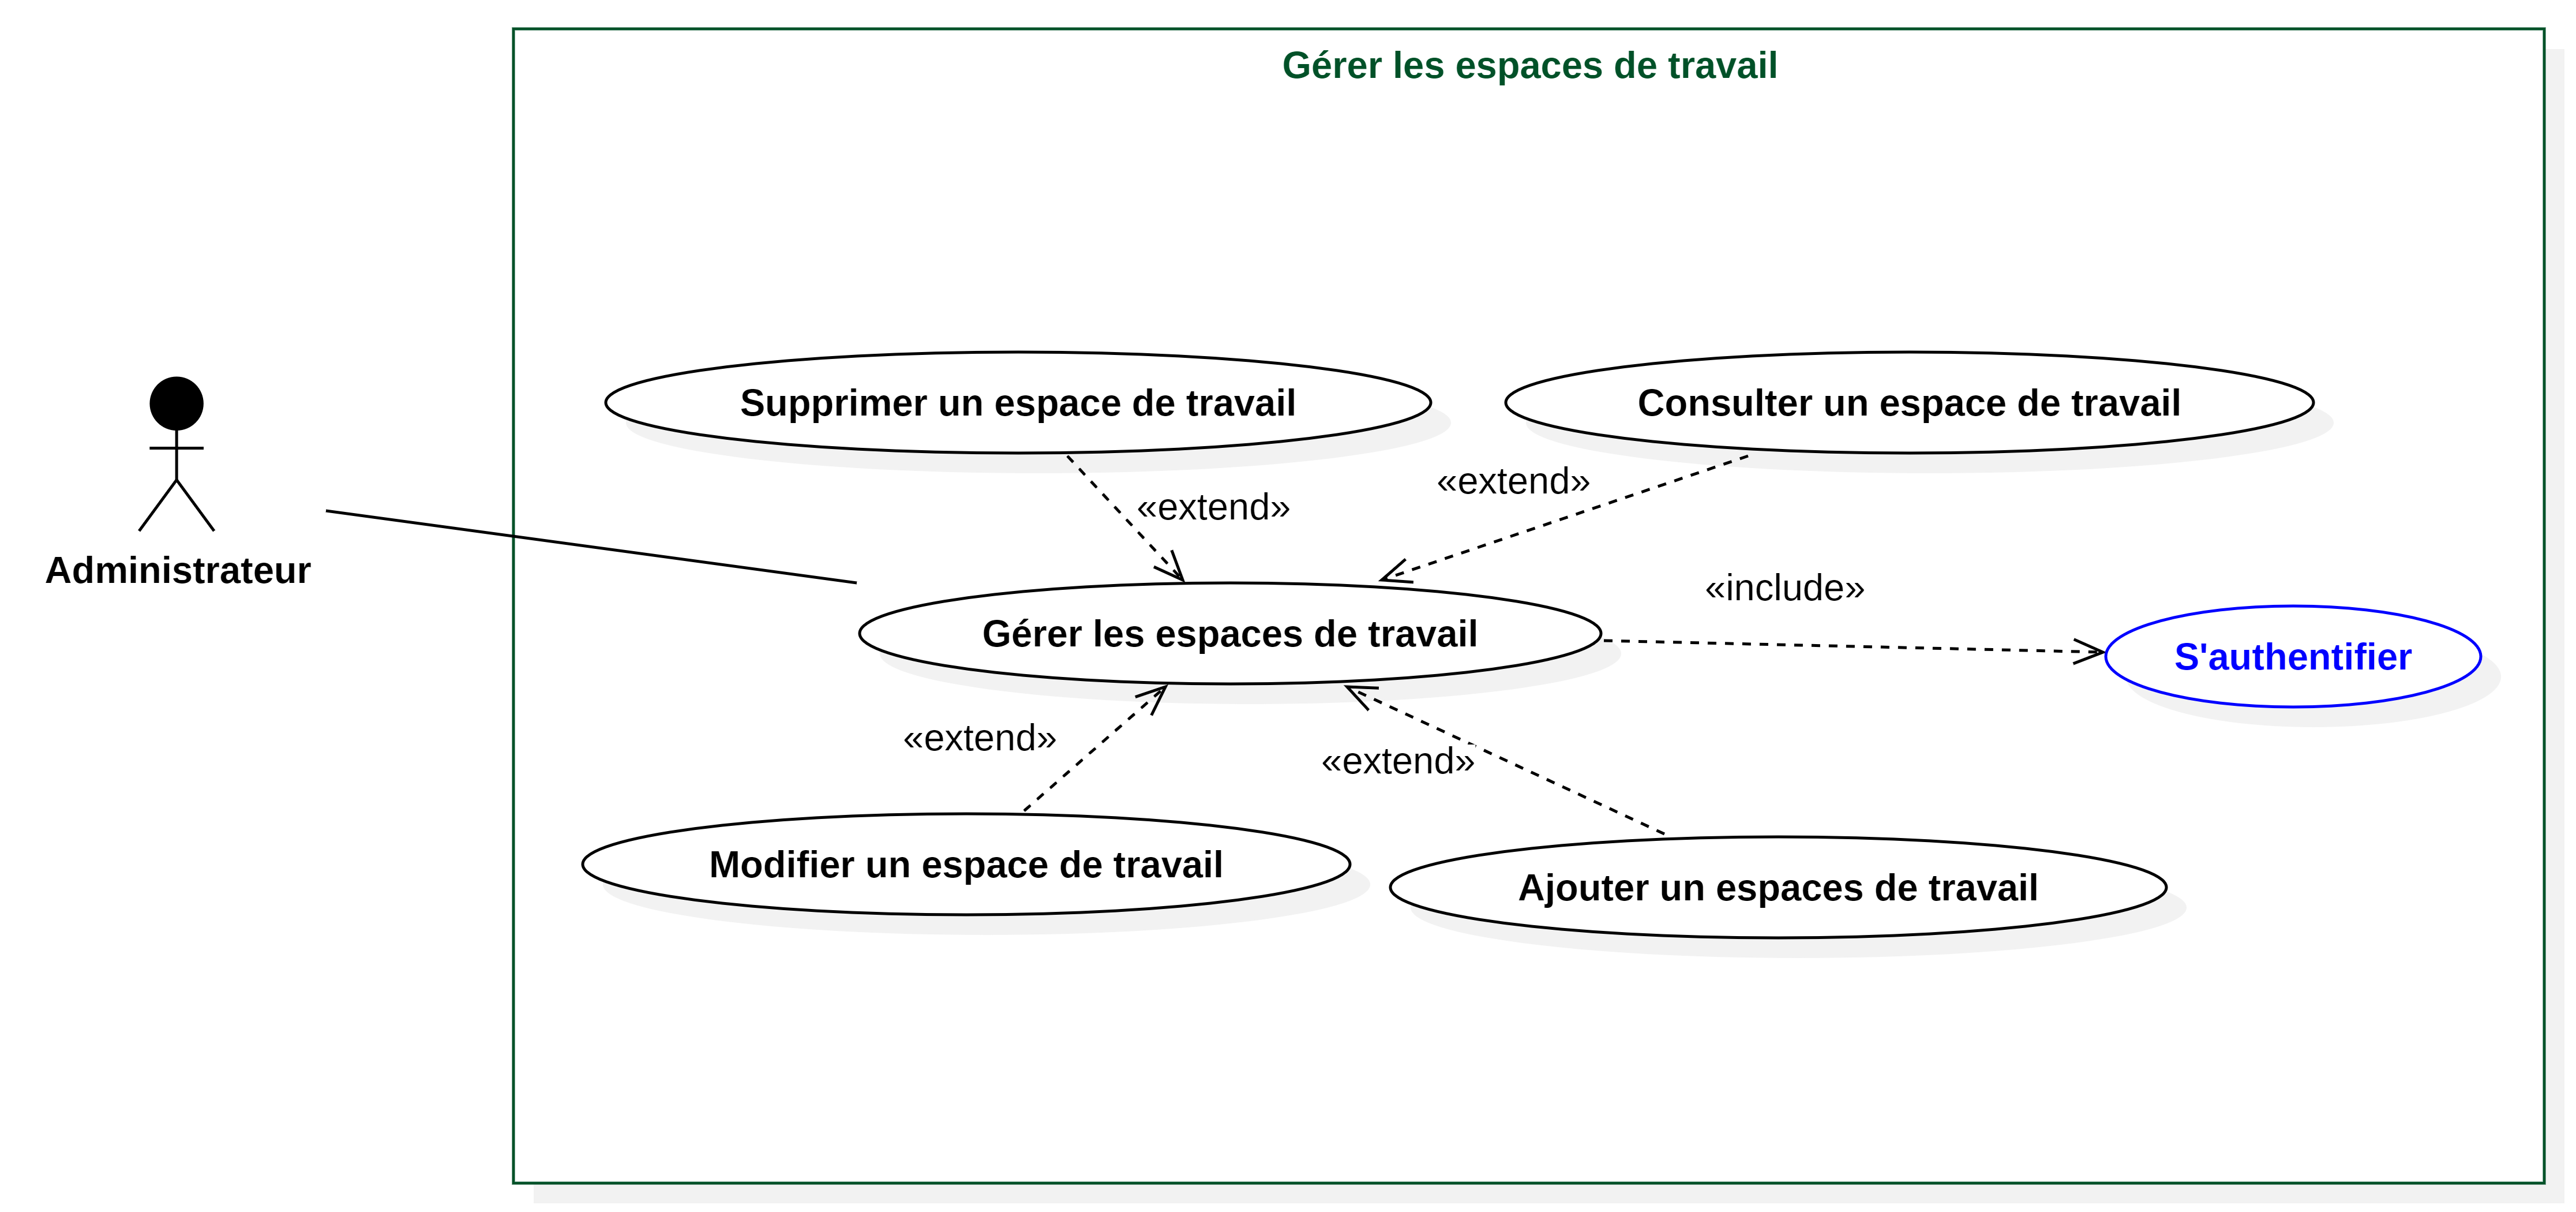
\includegraphics[width=1\columnwidth]{gereE.png}
  \caption{Diagramme de cas d'utilisation « Gestion des espaces de travail »}
  \label{fig:GestionWorkspaceUseCase}
\end{figure}

\begin{longtable}[c]{|p{0.3\linewidth}|p{0.65\linewidth}|}
  \hline
  \multicolumn{2}{|c|}{\textbf{Gérer un espace de travail}}                                                             \\
  \hline
  \endfirsthead

  \hline
  \multicolumn{2}{|c|}{\textbf{Gérer un espace de travail}}                                                             \\
  \hline
  \endhead

  \hline
  \endfoot

  \hline
  \endlastfoot

  \textbf{Objectif}      & Créer, consulter et organiser les espaces de travail de l'application.                       \\
  \hline
  \textbf{Acteur(s)}     & Administrateur, ProjectManager, Membre                                                       \\
  \hline
  \textbf{Précondition}  & L'utilisateur doit être authentifié.                                                         \\
  \hline
  \textbf{Scénario}      &
  1. L'utilisateur accède à la section des espaces de travail.                                                          \\
                         & 2. Le système affiche les espaces de travail accessibles.                                    \\
                         & 3. L'administrateur peut créer un nouvel espace de travail.                                  \\
                         & 4. L'administrateur ou le ProjectManager peut inviter des membres selon les droits accordés. \\
                         & 5. Le membre invité peut accepter ou refuser l'invitation reçue.                             \\
                         & 6. Le système met à jour la liste des membres de l'espace de travail.                        \\
  \hline
  \textbf{Postcondition} & L'espace de travail est créé ou mis à jour avec les membres concernés.                       \\
  \hline
  \caption{\centering Description textuelle du cas d'utilisation « Gérer un espace de travail »}
\end{longtable}
\subsection{Gestion des projets}

La figure \ref{fig:GestionProjetUseCase} ci-dessous illustre le diagramme de raffinement de la gestion des projets.

\begin{figure}[H]
  \centering
   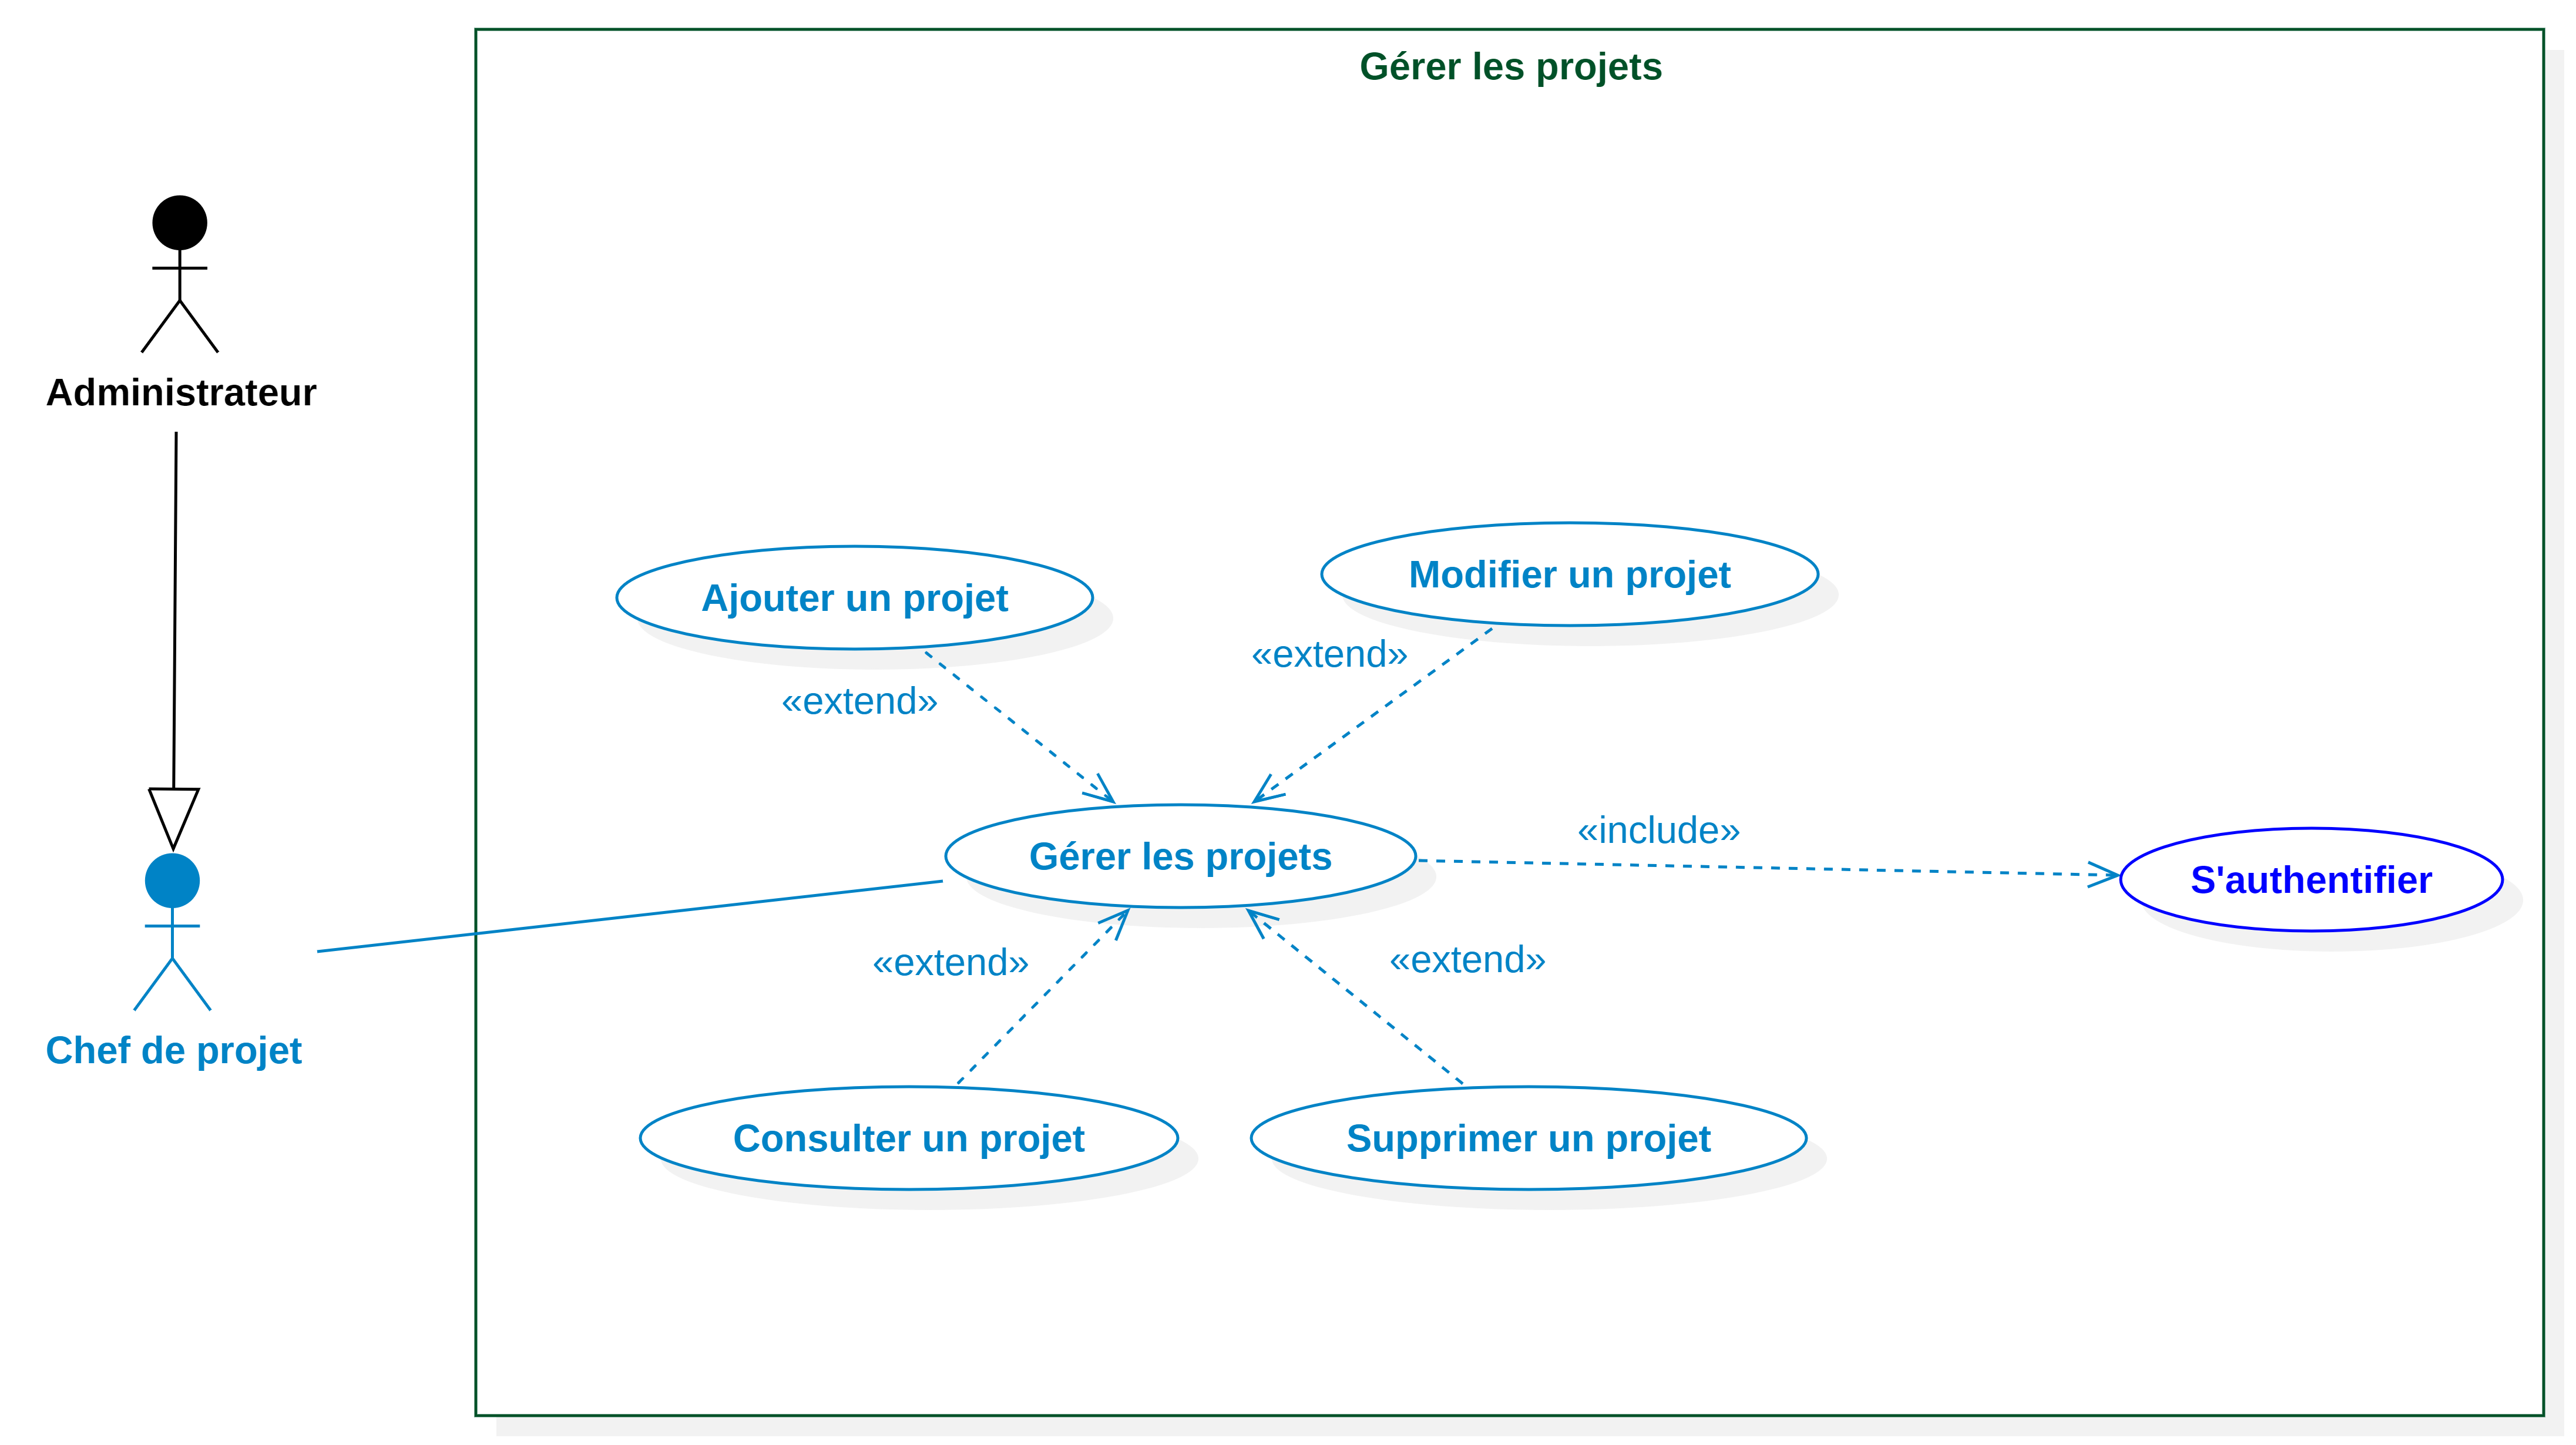
\includegraphics[width=1\columnwidth]{gereP.png}
  \caption{Diagramme de cas d'utilisation « Gestion des projets »}
  \label{fig:GestionProjetUseCase}
\end{figure}

\begin{longtable}[c]{|p{0.3\linewidth}|p{0.65\linewidth}|}
  \hline
  \multicolumn{2}{|c|}{\textbf{Gérer un projet}}                                                             \\
  \hline
  \endfirsthead

  \hline
  \multicolumn{2}{|c|}{\textbf{Gérer un projet}}                                                             \\
  \hline
  \endhead

  \hline
  \endfoot

  \hline
  \endlastfoot

  \textbf{Objectif}      & Permettre la création, la modification, la suppression et le suivi des projets.                   \\
  \hline
  \textbf{Acteur(s)}     & Administrateur, ProjectManager, Membre                                            \\
  \hline
  \textbf{Précondition}  & L'utilisateur doit être authentifié et appartenir à l'espace de travail concerné. \\
  \hline
  \textbf{Scénario}      &
  1. L'utilisateur accède à la liste des projets.                                                            \\
                         & 2. Le système affiche les projets accessibles.                                    \\
                         & 3. Le ProjectManager crée ou modifie un projet.                                   \\
                         & 4. Le ProjectManager invite des membres à rejoindre le projet.                    \\
                         & 5. Les membres acceptent ou refusent l'invitation.                                \\
                         & 6. Le système met à jour les informations du projet et sa liste des membres.      \\
  \hline
  \textbf{Postcondition} & Le projet est créé, modifié ou mis à jour avec les membres affectés.              \\
  \hline
  \caption{\centering Description textuelle du cas d'utilisation « Gérer un projet »}
\end{longtable}
\subsection{Gestion du backlog, des tâches et des sprints}

La figure \ref{fig:GestionBacklogSprintUseCase} ci-dessous illustre le diagramme de raffinement de la gestion du backlog, des tâches et des sprints.

\begin{figure}[H]
  \centering
  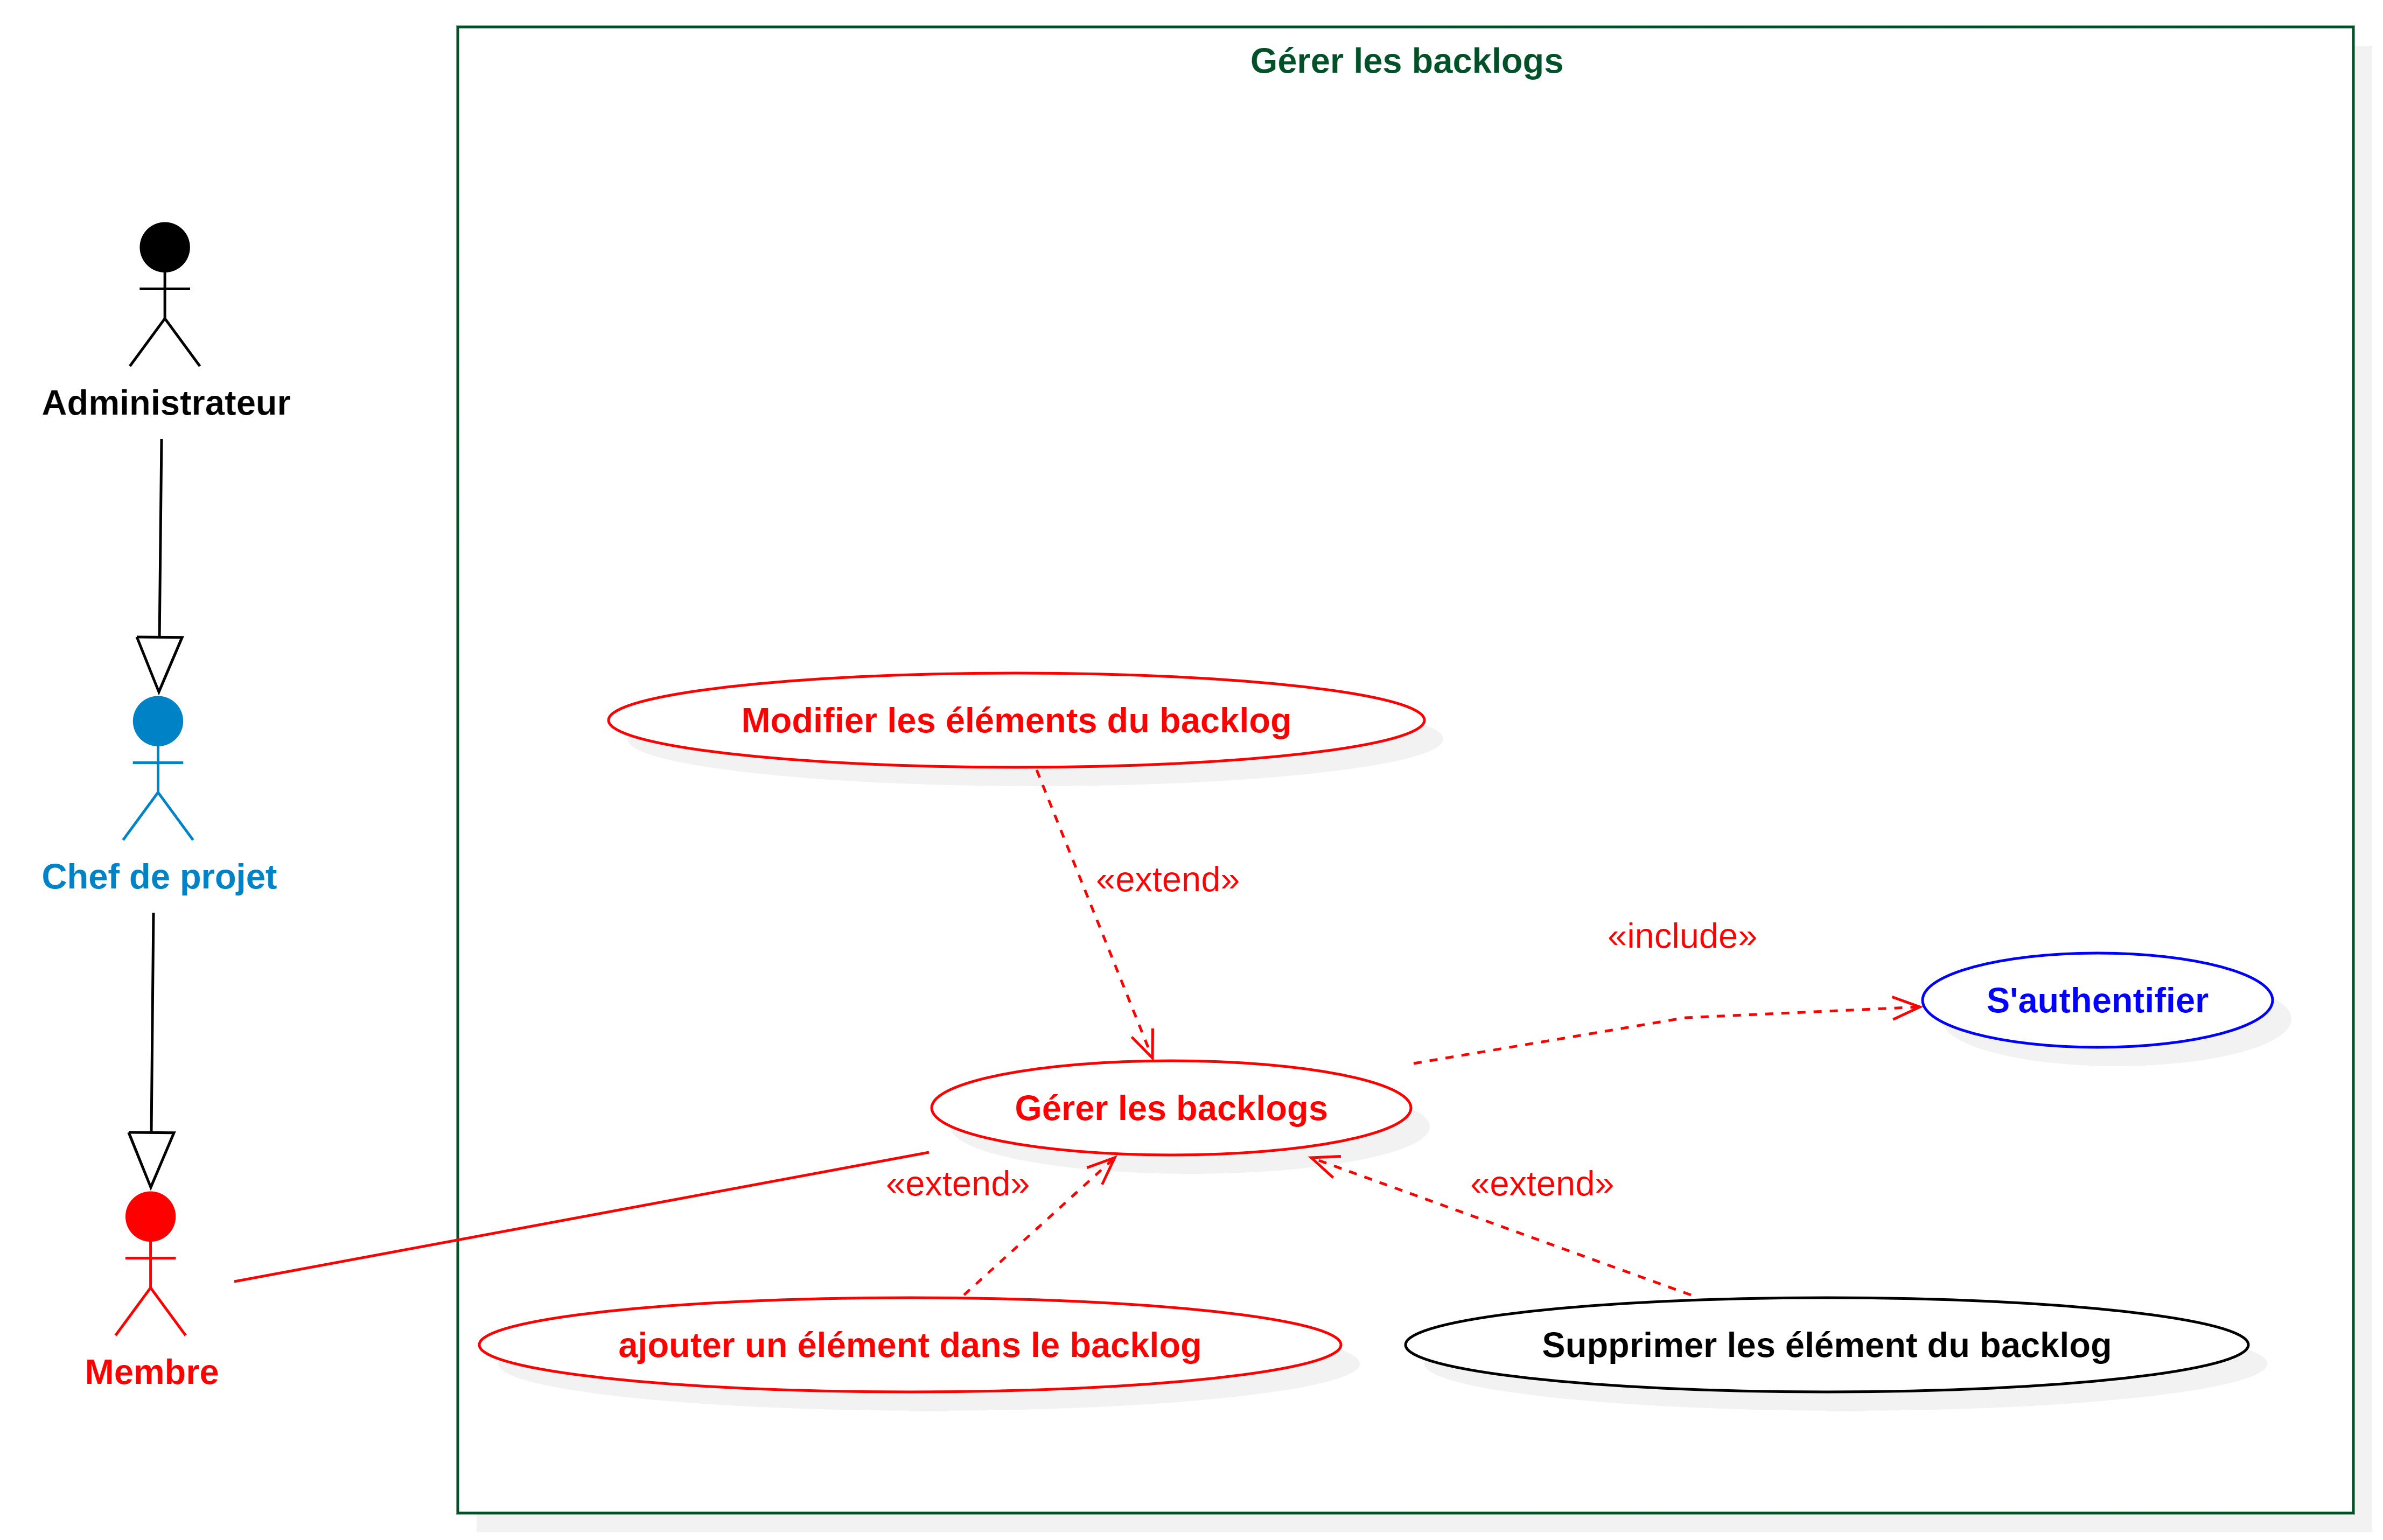
\includegraphics[width=1\columnwidth]{gereB.png}
  \caption{Diagramme de cas d'utilisation « Gestion du backlog, des tâches et des sprints »}
  \label{fig:GestionBacklogSprintUseCase}
\end{figure}

\begin{longtable}[c]{|p{0.3\linewidth}|p{0.65\linewidth}|}
  \hline
  \multicolumn{2}{|c|}{\textbf{Gérer le backlog et les sprints}}                                                                                              \\
  \hline
  \endfirsthead

  \hline
  \multicolumn{2}{|c|}{\textbf{Gérer le backlog et les sprints}}                                                                                              \\
  \hline
  \endhead

  \hline
  \endfoot

  \hline
  \endlastfoot

  \textbf{Objectif}      & Organiser les éléments du backlog, les tâches et les sprints d'un projet.                                                          \\
  \hline
  \textbf{Acteur(s)}     & ProjectManager, Membre                                                                                                             \\
  \hline
  \textbf{Précondition}  & L'utilisateur doit être authentifié et avoir accès au projet concerné.                                                             \\
  \hline
  \textbf{Scénario}      &
  1. L'utilisateur accède au backlog du projet.                                                                                                               \\
                         & 2. Le système affiche les éléments du backlog existants.                                                                           \\
                         & 3. L'utilisateur peut créer, modifier ou supprimer un élément du backlog.                                                          \\
                         & 4. L'utilisateur peut affecter un élément à un membre, définir sa priorité, sa complexité, ses story points et sa date d'échéance. \\
                         & 5. L'utilisateur crée un sprint et y associe des éléments du backlog.                                                              \\
                         & 6. Le système met à jour l'état d'avancement des tâches et des sprints.                                                            \\
  \hline
  \textbf{Postcondition} & Le backlog, les tâches ou les sprints sont mis à jour selon les actions effectuées.                                                \\
  \hline
  \caption{\centering Description textuelle du cas d'utilisation « Gérer le backlog et les sprints »}
\end{longtable}
\subsection{Gestion de la collaboration et des réunions}

La figure \ref{fig:GestionCollaborationUseCase} ci-dessous illustre le diagramme de raffinement de la gestion de la collaboration et des réunions.

\begin{figure}[H]
  \centering
   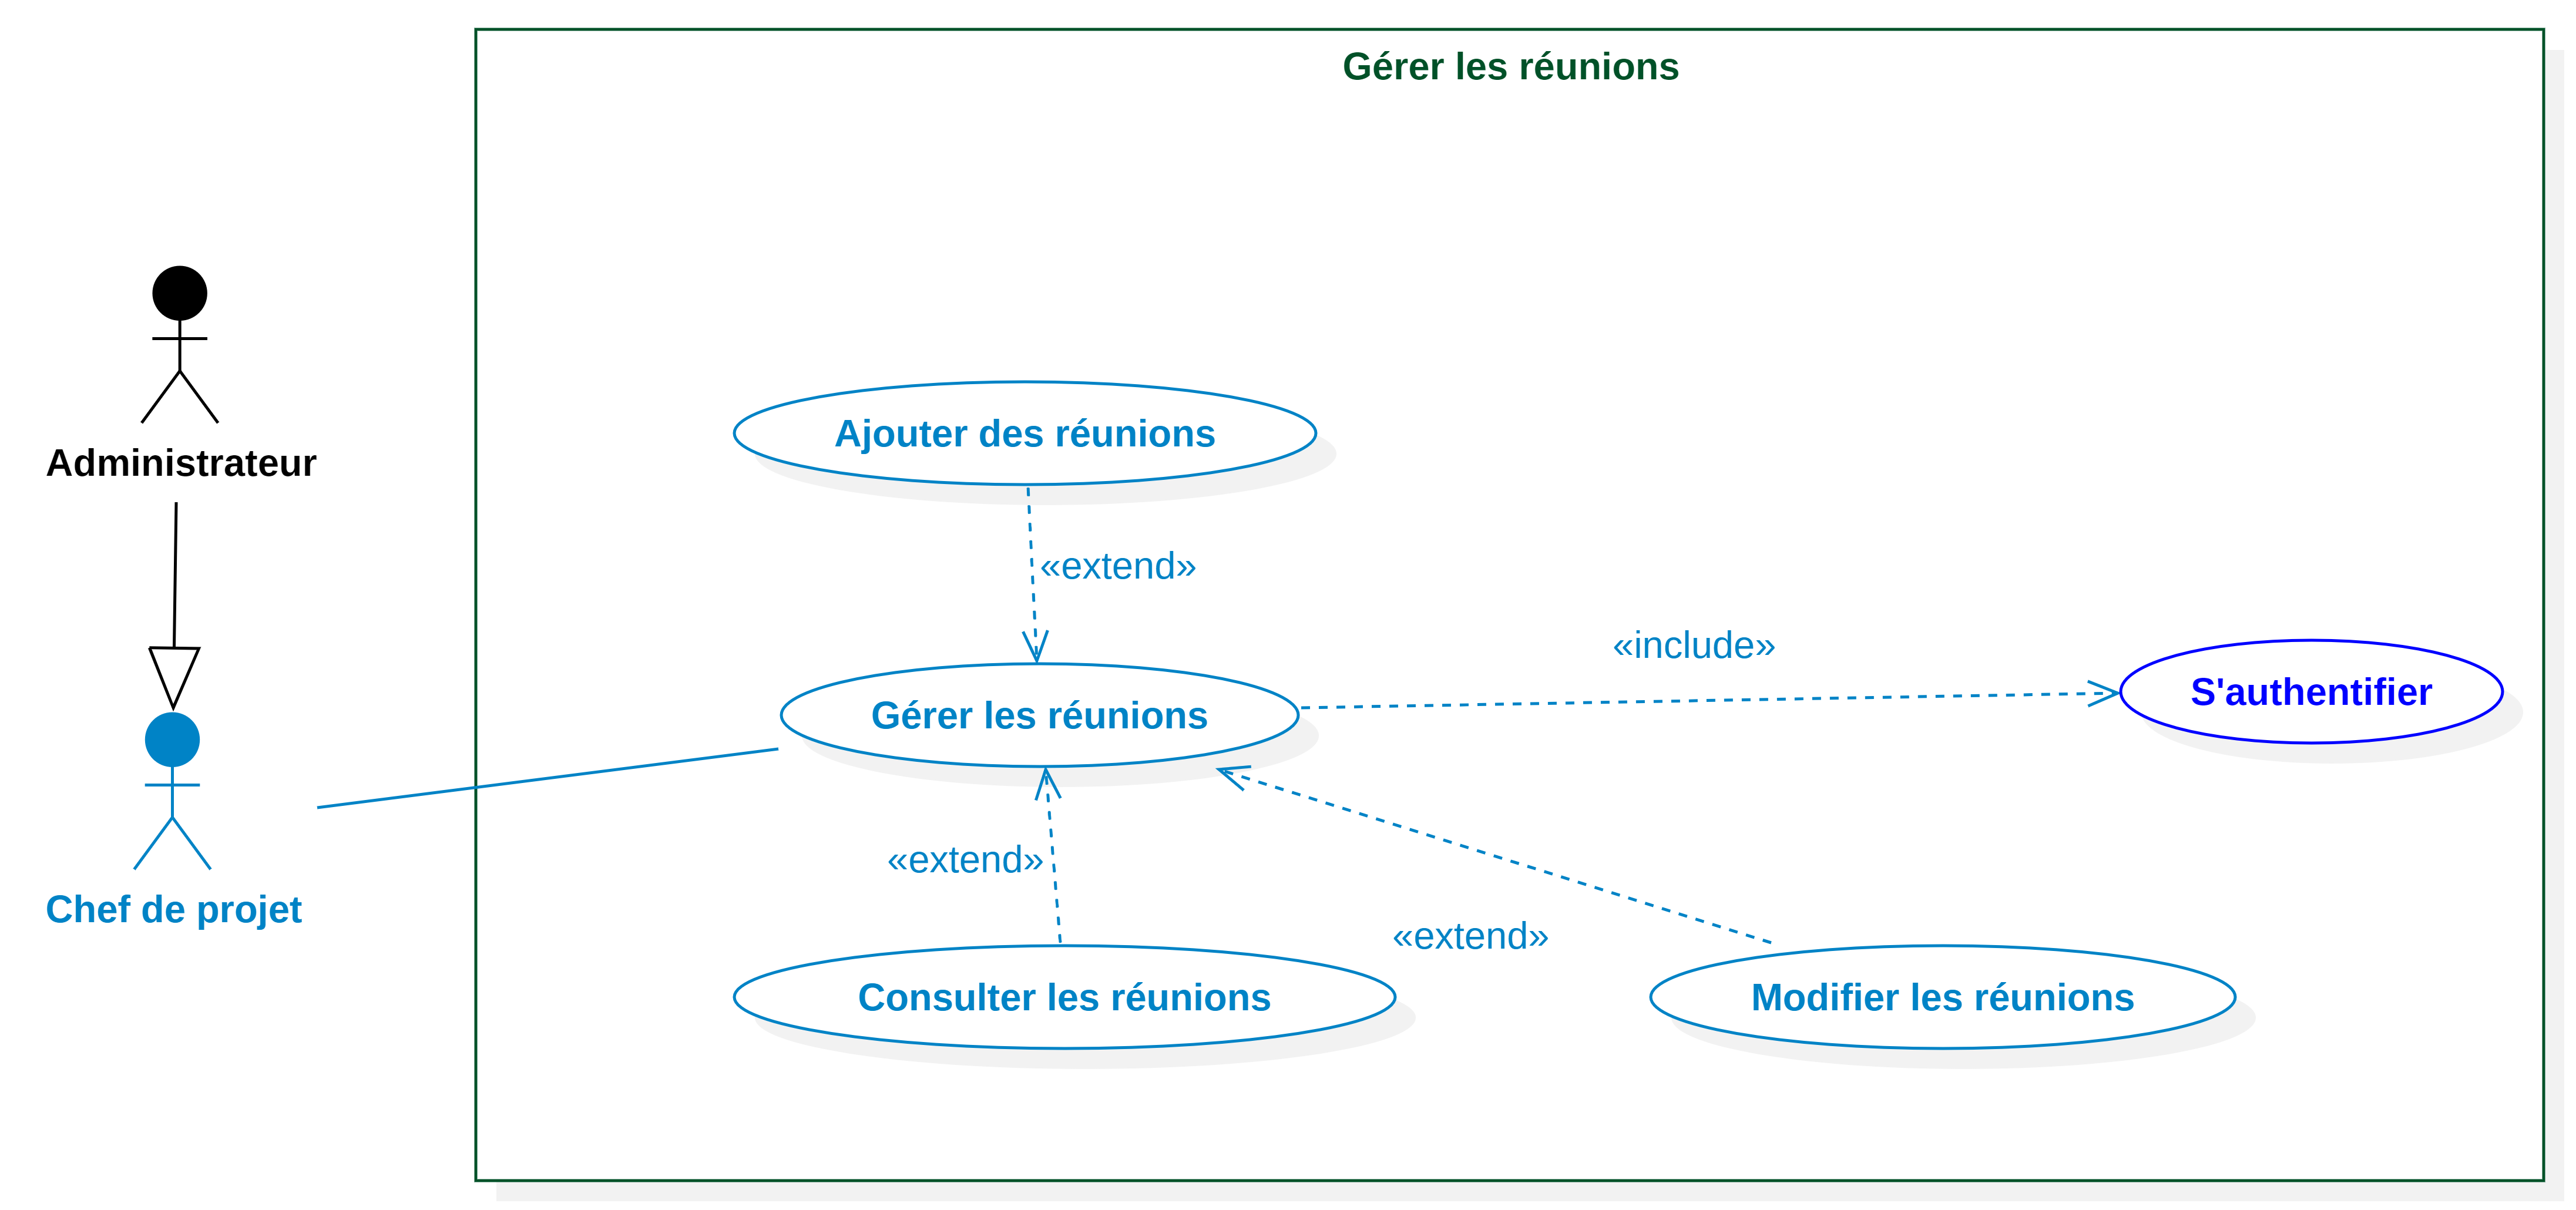
\includegraphics[width=1\columnwidth]{gereR.png}
  \caption{Diagramme de cas d'utilisation « Gestion de la collaboration et des réunions »}
  \label{fig:GestionCollaborationUseCase}
\end{figure}

\begin{longtable}[c]{|p{0.3\linewidth}|p{0.65\linewidth}|}
  \hline
  \multicolumn{2}{|c|}{\textbf{Collaborer au sein d'un projet}}                                                               \\
  \hline
  \endfirsthead

  \hline
  \multicolumn{2}{|c|}{\textbf{Collaborer au sein d'un projet}}                                                               \\
  \hline
  \endhead

  \hline
  \endfoot

  \hline
  \endlastfoot

  \textbf{Objectif}      & Faciliter la communication entre les membres d'un projet et organiser les réunions.                \\
  \hline
  \textbf{Acteur(s)}     & ProjectManager, Membre                                                                             \\
  \hline
  \textbf{Précondition}  & L'utilisateur doit être authentifié et appartenir au projet concerné.                              \\
  \hline
  \textbf{Scénario}      &
  1. L'utilisateur accède à l'espace de discussion du projet.                                                                 \\
                         & 2. Le système affiche les conversations associées au projet.                                       \\
                         & 3. L'utilisateur envoie ou consulte les messages échangés avec les membres.                        \\
                         & 4. L'utilisateur peut consulter les réunions planifiées dans le calendrier.                        \\
                         & 5. Le ProjectManager peut créer une réunion et définir les membres concernés.                      \\
                         & 6. Le système enregistre la réunion et l'affiche dans le calendrier.                               \\
  \hline
  \textbf{Postcondition} & Les messages ou les réunions du projet sont enregistrés et consultables par les membres concernés. \\
  \hline
  \caption{\centering Description textuelle du cas d'utilisation « Collaborer au sein d'un projet »}
\end{longtable}
\subsection{Suivi de la santé de l'équipe}

La figure \ref{fig:TeamHealthUseCase} ci-dessous illustre le diagramme de raffinement du suivi de la santé de l'équipe.

\begin{figure}[H]
  \centering
   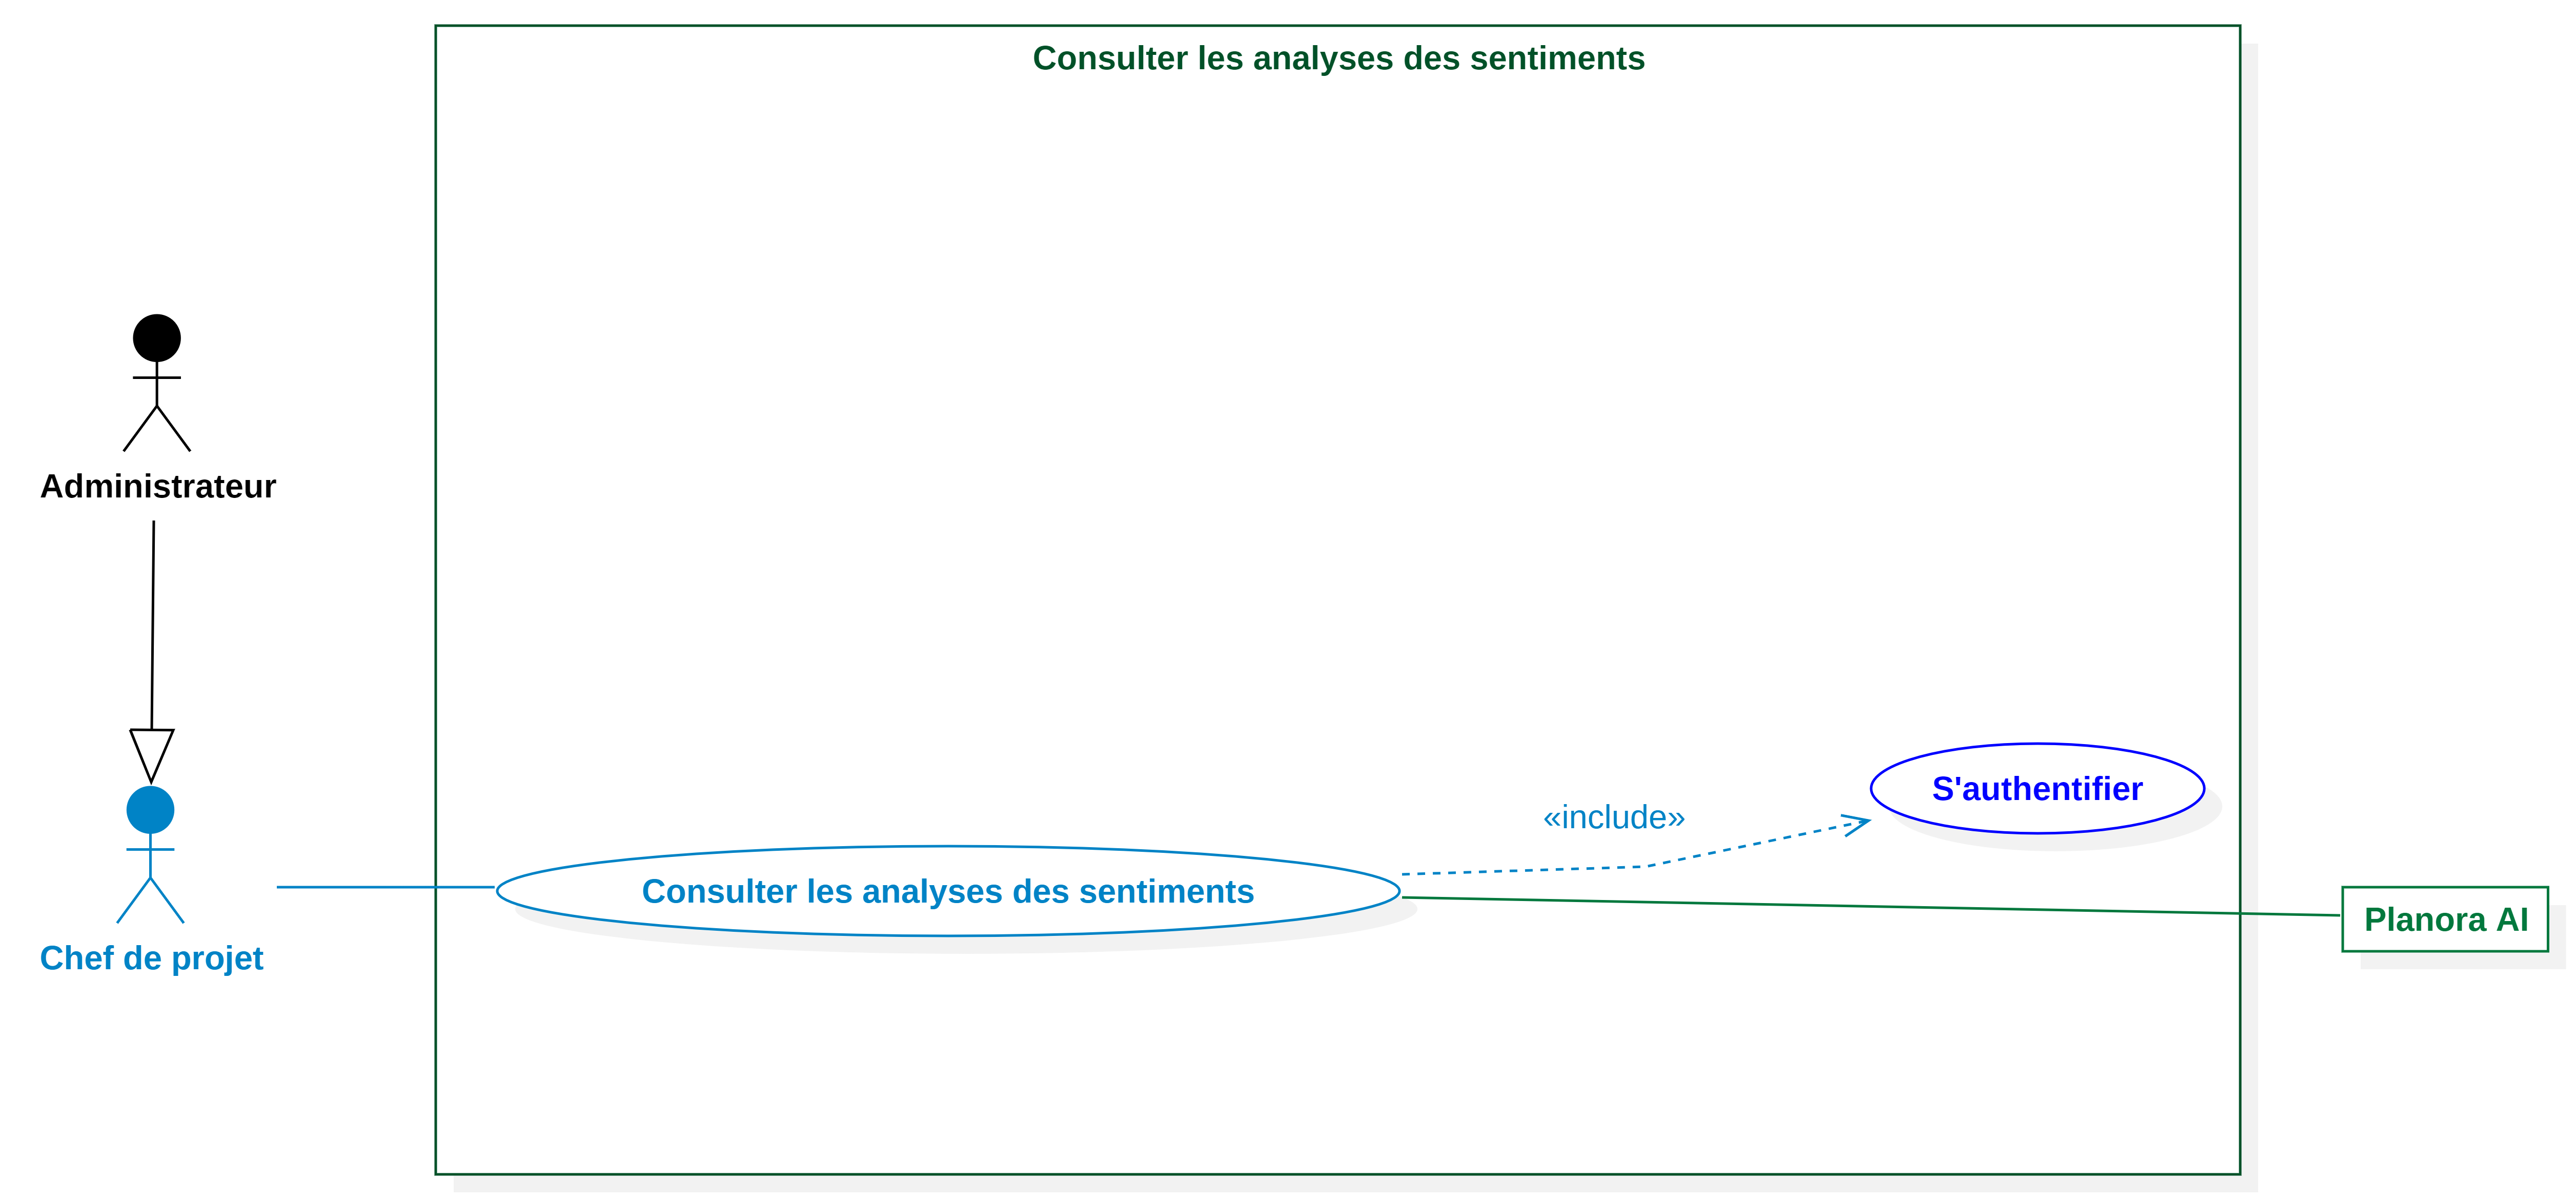
\includegraphics[width=1\columnwidth]{ConsAi.png}
  \caption{Diagramme de cas d'utilisation « Suivi de la santé de l'équipe »}
  \label{fig:TeamHealthUseCase}
\end{figure}

\begin{longtable}[c]{|p{0.3\linewidth}|p{0.65\linewidth}|}
  \hline
  \multicolumn{2}{|c|}{\textbf{Analyser la santé de l'équipe}}                                                           \\
  \hline
  \endfirsthead

  \hline
  \multicolumn{2}{|c|}{\textbf{Analyser la santé de l'équipe}}                                                           \\
  \hline
  \endhead

  \hline
  \endfoot

  \hline
  \endlastfoot

  \textbf{Objectif}      & Analyser les messages échangés afin d'évaluer l'ambiance générale de l'équipe.                \\
  \hline
  \textbf{Acteur(s)}     & ProjectManager, Membre                                                                        \\
  \hline
  \textbf{Précondition}  & L'utilisateur doit être authentifié et avoir accès au projet concerné.                        \\
  \hline
  \textbf{Scénario}      &
  1. L'utilisateur accède à la page de suivi de la santé de l'équipe.                                                    \\
                         & 2. Le système récupère les messages récents échangés dans le projet.                          \\
                         & 3. Le module d'intelligence artificielle analyse les messages.                                \\
                         & 4. Le système classe les messages selon leur sentiment : positif, neutre, stressé ou frustré. \\
                         & 5. Le système calcule un score global et affiche les indicateurs de santé de l'équipe.        \\
                         & 6. En cas de stress ou de frustration élevés, le système affiche des alertes.                 \\
  \hline
  \textbf{Postcondition} & Les indicateurs et alertes liés à la santé de l'équipe sont affichés à l'utilisateur.         \\
  \hline
  \caption{\centering Description textuelle du cas d'utilisation « Analyser la santé de l'équipe »}
\end{longtable}
\subsection{Communication entre les membres d'un projet}

La figure \ref{fig:TeamHealthUseCase} ci-dessous illustre le diagramme de raffinement du communication entre les memebres d'un projet.

\begin{figure}[H]
  \centering
   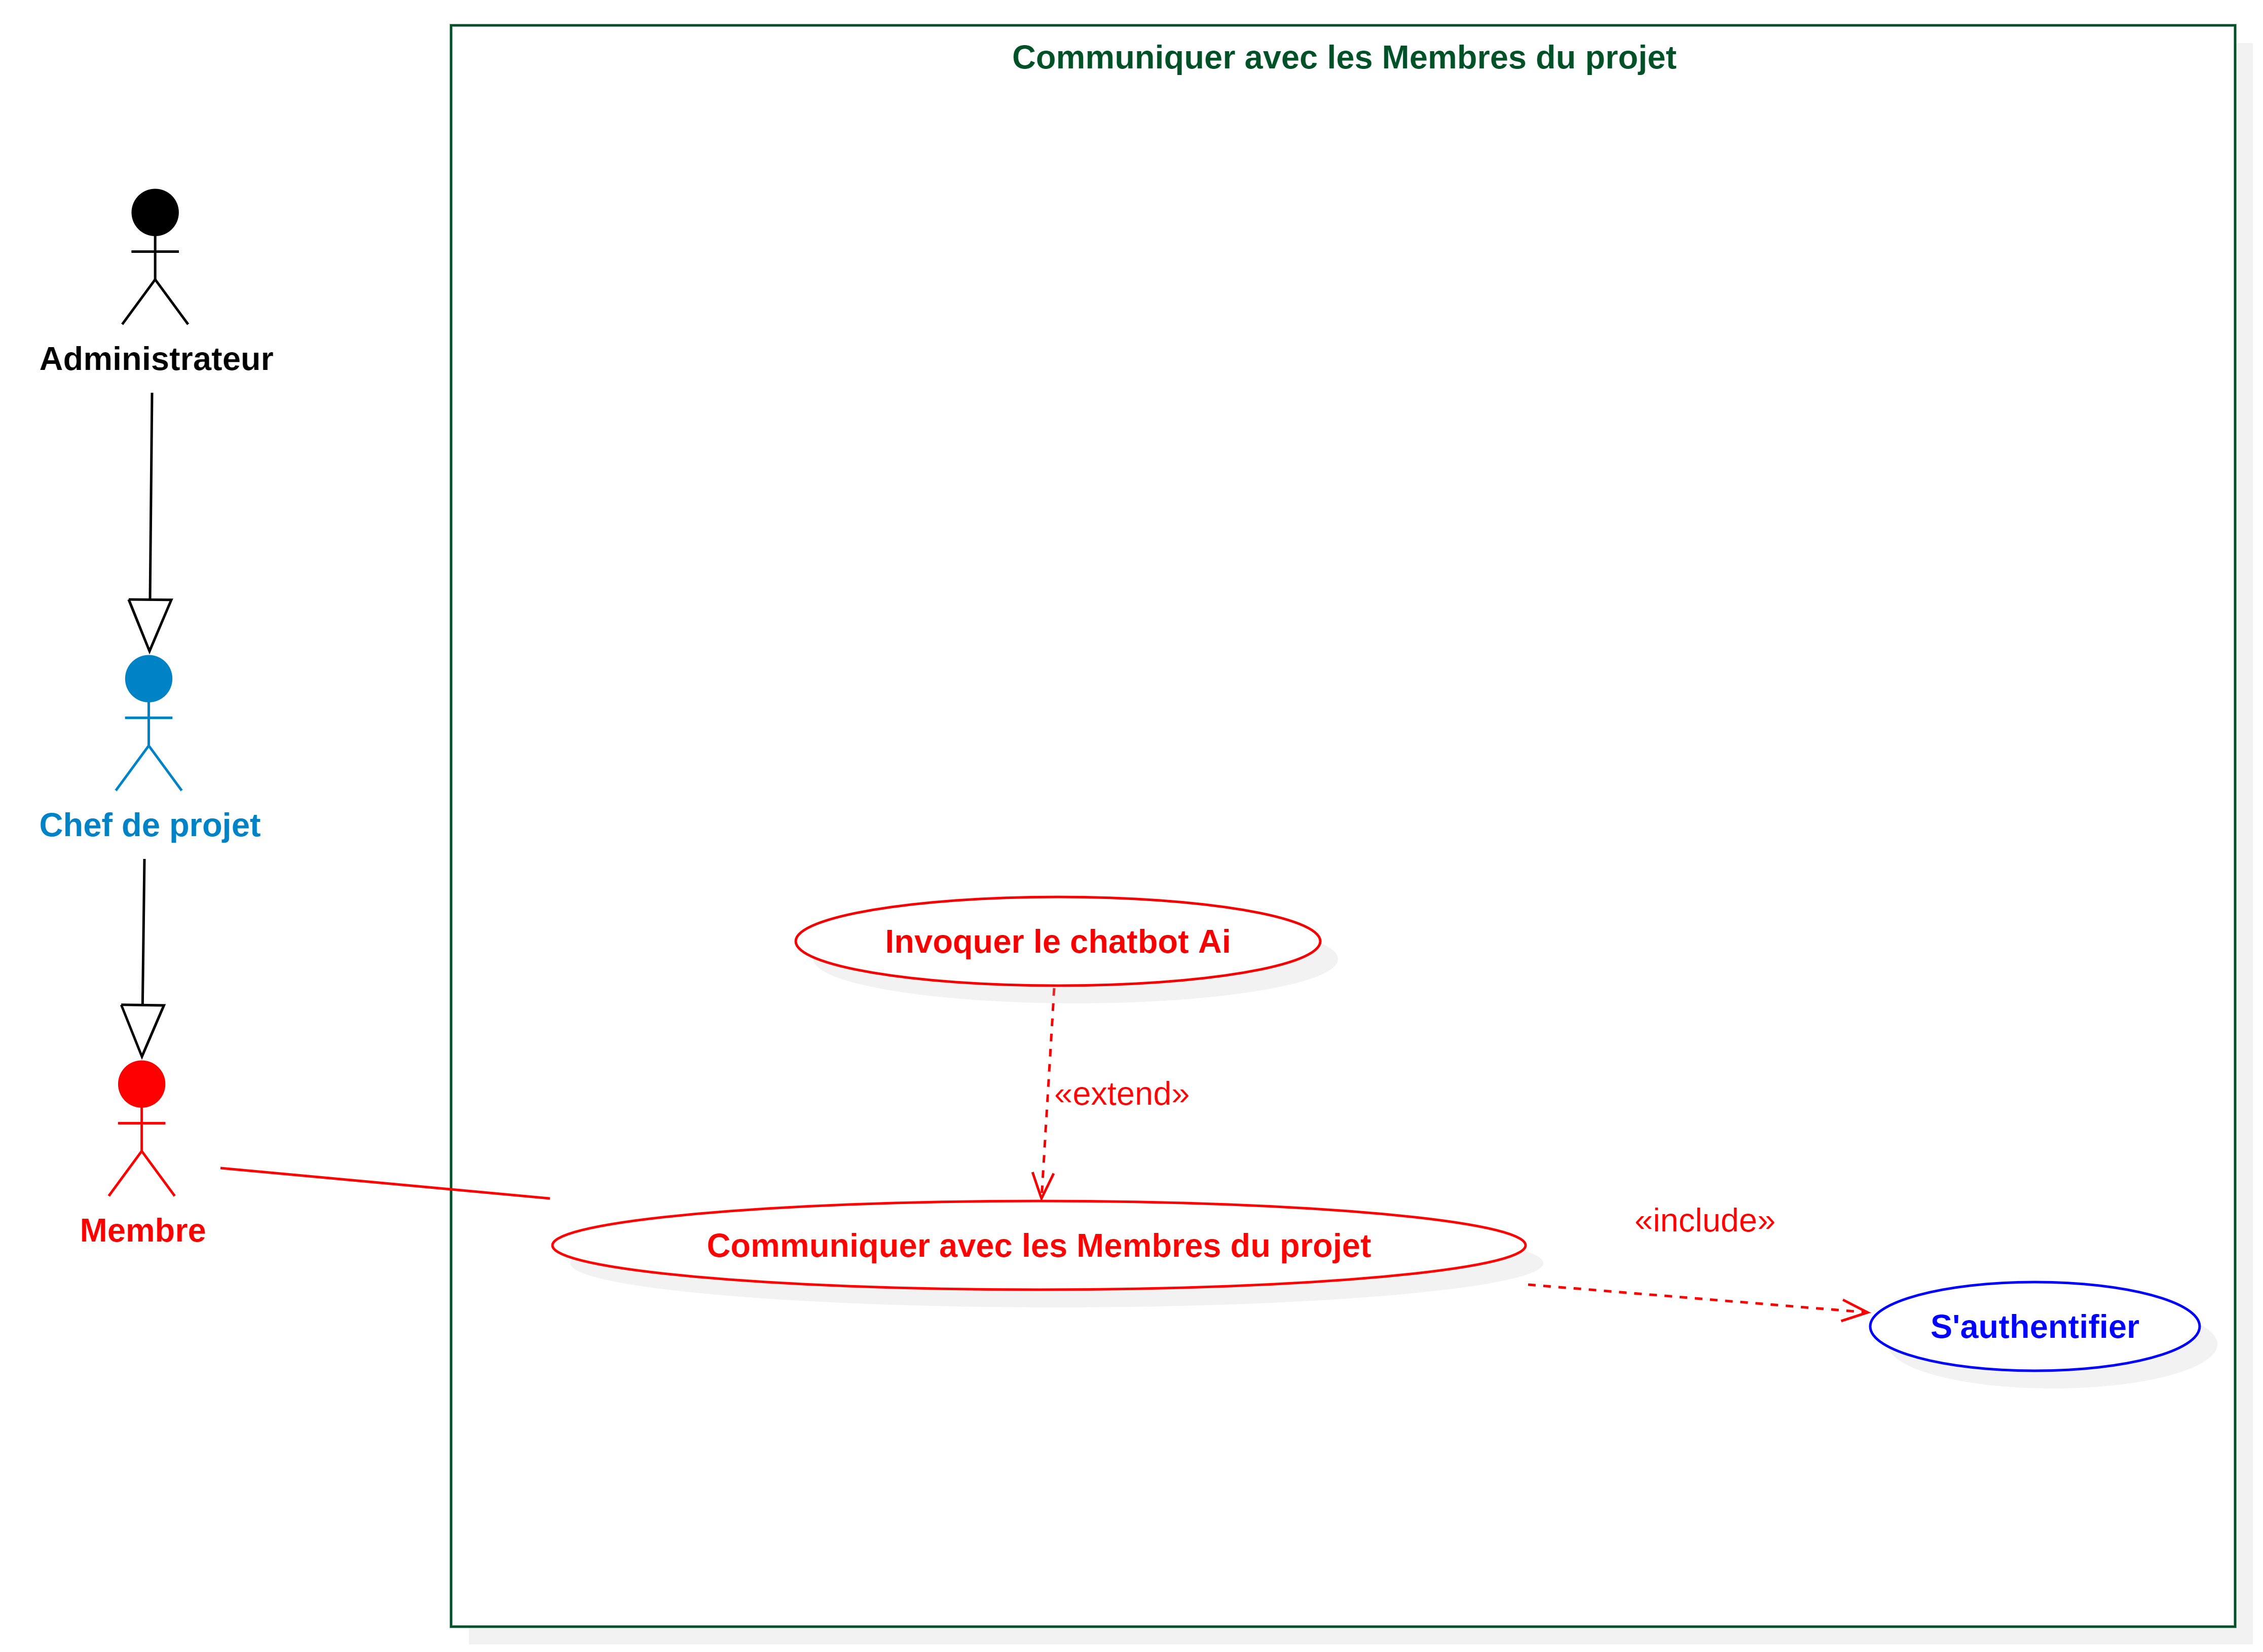
\includegraphics[width=1\columnwidth]{ComAi.png}
  \caption{Diagramme de cas d'utilisation « Communication entre les membres d'un projet »}
  \label{fig:TeamHealthUseCase}
\end{figure}

\begin{longtable}[c]{|p{0.3\linewidth}|p{0.65\linewidth}|}
  \hline
  \multicolumn{2}{|c|}{\textbf{Communication entre les membres d'un projet}}                                                           \\
  \hline
  \endfirsthead

  \hline
  \multicolumn{2}{|c|}{\textbf{Communication entre les membres d'un projet}}                                                           \\
  \hline
  \endhead

  \hline
  \endfoot

  \hline
  \endlastfoot

  \textbf{Objectif}      & Analyser les messages échangés afin d'évaluer l'ambiance générale de l'équipe.                \\
  \hline
  \textbf{Acteur(s)}     & Admin, ProjectManager, Membre                                                                        \\
  \hline
  \textbf{Précondition}  & L'utilisateur doit être authentifié et avoir accès au projet concerné.                        \\
  \hline
  \textbf{Scénario}      &
  1. L'utilisateur accède à la page de suivi de la santé de l'équipe.                                                    \\
                         & 2. Le système récupère les messages récents échangés dans le projet.                          \\
                         & 3. Le module d'intelligence artificielle analyse les messages.                                \\
                         & 4. Le système classe les messages selon leur sentiment : positif, neutre, stressé ou frustré. \\
                         & 5. Le système calcule un score global et affiche les indicateurs de santé de l'équipe.        \\
                         & 6. En cas de stress ou de frustration élevés, le système affiche des alertes.                 \\
  \hline
  \textbf{Postcondition} & Les indicateurs et alertes liés à la santé de l'équipe sont affichés à l'utilisateur.         \\
  \hline
  \caption{\centering Description textuelle du cas d'utilisation « Analyser la santé de l'équipe »}
\end{longtable}


\section*{Conclusion}


Dans le deuxième chapitre, nous avons nous avons effectué une analyse et une spécification des besoins en identifiant les acteurs clés du projet.Ensuite nous avons défini les exigences fonctionnelles et non fonctionnelles. Enfin, nous avons présenté une illustration du diagramme d'utilisation global ainsi que ses raffinements.


%%%%% Chapter three
\chapter{Conception}

\section*{Introduction}
Dans ce chapitre, nous explorons les différentes fonctionnalités de l'application à travers des diagrammes de classe et de séquences, décrivant ainsi la structure et les interactions entre les différents acteurs de l'application.

\section{Outil de conception}
\subsection{StarUML}
StarUML, développé par MKLab, est un outil de modélisation UML puissant et convivial. Il offre une interface intuitive pour créer des diagrammes de classe, de séquence et d'autres types de diagrammes UML. StarUML prend en charge la génération de code à partir des diagrammes, facilitant ainsi la transition entre la conception et le développement. \cite{StarUML}
La figure \ref{StarUML} ci-dessous illustre la méthodologie hybride adoptée :
\begin{figure}[H]
  \centering
  
\includegraphics[width=0.12\columnwidth]{Staruml_logo.png}
  \caption{Logo de StarUML}
  \label{StarUML}
\end{figure}
\section{Conception détaillée}

\subsection{Diagramme de classes général}

Le diagramme de classes général de l'application Planora est élaboré à partir des entités du domaine définies dans le backend. Il permet de représenter la structure principale du système ainsi que les relations entre les utilisateurs, les espaces de travail, les projets, les tâches, le backlog, les sprints, la messagerie et les réunions.

Le diagramme de classes général comprend principalement :
\begin{itemize}
  \item[$\bullet$] \textbf{Classe "Users"} : Représente l'utilisateur de l'application. Elle contient les informations personnelles de l'utilisateur, son état d'activation, son jeton de rafraîchissement ainsi que ses relations avec les workspaces, les projets, les espaces de travail, les tâches, les commentaires, les messages et les sessions de discussion.

  \item[$\bullet$] \textbf{Classe "Workspace"} : Représente un espace de travail. Elle contient le nom, la description, le propriétaire, le ProjectManager, les membres, les projets associés et les invitations envoyées.

  \item[$\bullet$] \textbf{Classe "Project"} : Représente un projet appartenant à un espace de travail. Elle contient le nom, la description, les dates de début et de fin, le ProjectManager, les membres du projet, les sprints, les éléments du backlog et les sessions de discussion.

  \item[$\bullet$] \textbf{Classe "BacklogItem"} : Représente un élément du backlog. Elle contient le titre, la description, la priorité, le statut, la complexité, les story points, la date d'échéance, le sprint associé et l'utilisateur assigné.

  \item[$\bullet$] \textbf{Classe "SubTask"} : Représente une sous-tâche liée à un élément du backlog. Elle contient le titre, l'état d'achèvement et l'identifiant de l'élément du backlog associé.

  \item[$\bullet$] \textbf{Classe "Sprint"} : Représente une itération de travail. Elle contient le nom, l'objectif, les dates de début et de fin, le statut, le projet associé et les tâches incluses dans le sprint.

  \item[$\bullet$] \textbf{Classe "TaskItem"} : Représente une tâche du projet. Elle contient le titre, la description, le statut, la priorité, le pourcentage d'avancement, la date d'échéance, le projet, le sprint et l'utilisateur assigné.

  \item[$\bullet$] \textbf{Classe "Comment"} : Représente un commentaire rédigé par un utilisateur. Il peut être associé soit à une tâche, soit à un élément du backlog.

  \item[$\bullet$] \textbf{Classe "ChatSession"} : Représente une session de discussion liée à un projet. Elle contient le titre, le créateur de la session et la collection des messages associés.

  \item[$\bullet$] \textbf{Classe "ChatMessage"} : Représente un message envoyé dans une session de discussion. Elle contient le contenu, l'expéditeur, le type du message, les informations de modification, les pièces jointes et les réactions.

  \item[$\bullet$] \textbf{Classe "MeetingEvent"} : Représente une réunion planifiée. Elle contient le projet concerné, le titre, la date de planification, le créateur, l'option de réunion en ligne et les membres visibles.

  \item[$\bullet$] \textbf{Classe "DailyCheckIn"} : Représente le suivi quotidien d'un membre. Elle contient le niveau d'énergie, les heures disponibles, l'existence d'un blocage, une note éventuelle, l'utilisateur et le projet concernés.

  \item[$\bullet$] \textbf{Classes "BacklogAttachment", "BacklogBranch", "BacklogCommit", "BacklogLink" et "BacklogWebLink"} : Représentent les éléments complémentaires liés au backlog, tels que les pièces jointes, les branches, les commits, les liens entre éléments du backlog et les liens web externes.
\end{itemize}
\newpage
La figure \ref{fig:DiagrammeClasseGeneral} illustre le diagramme de classes général de l'application Planora.

\begin{figure}[H]
  \centering
  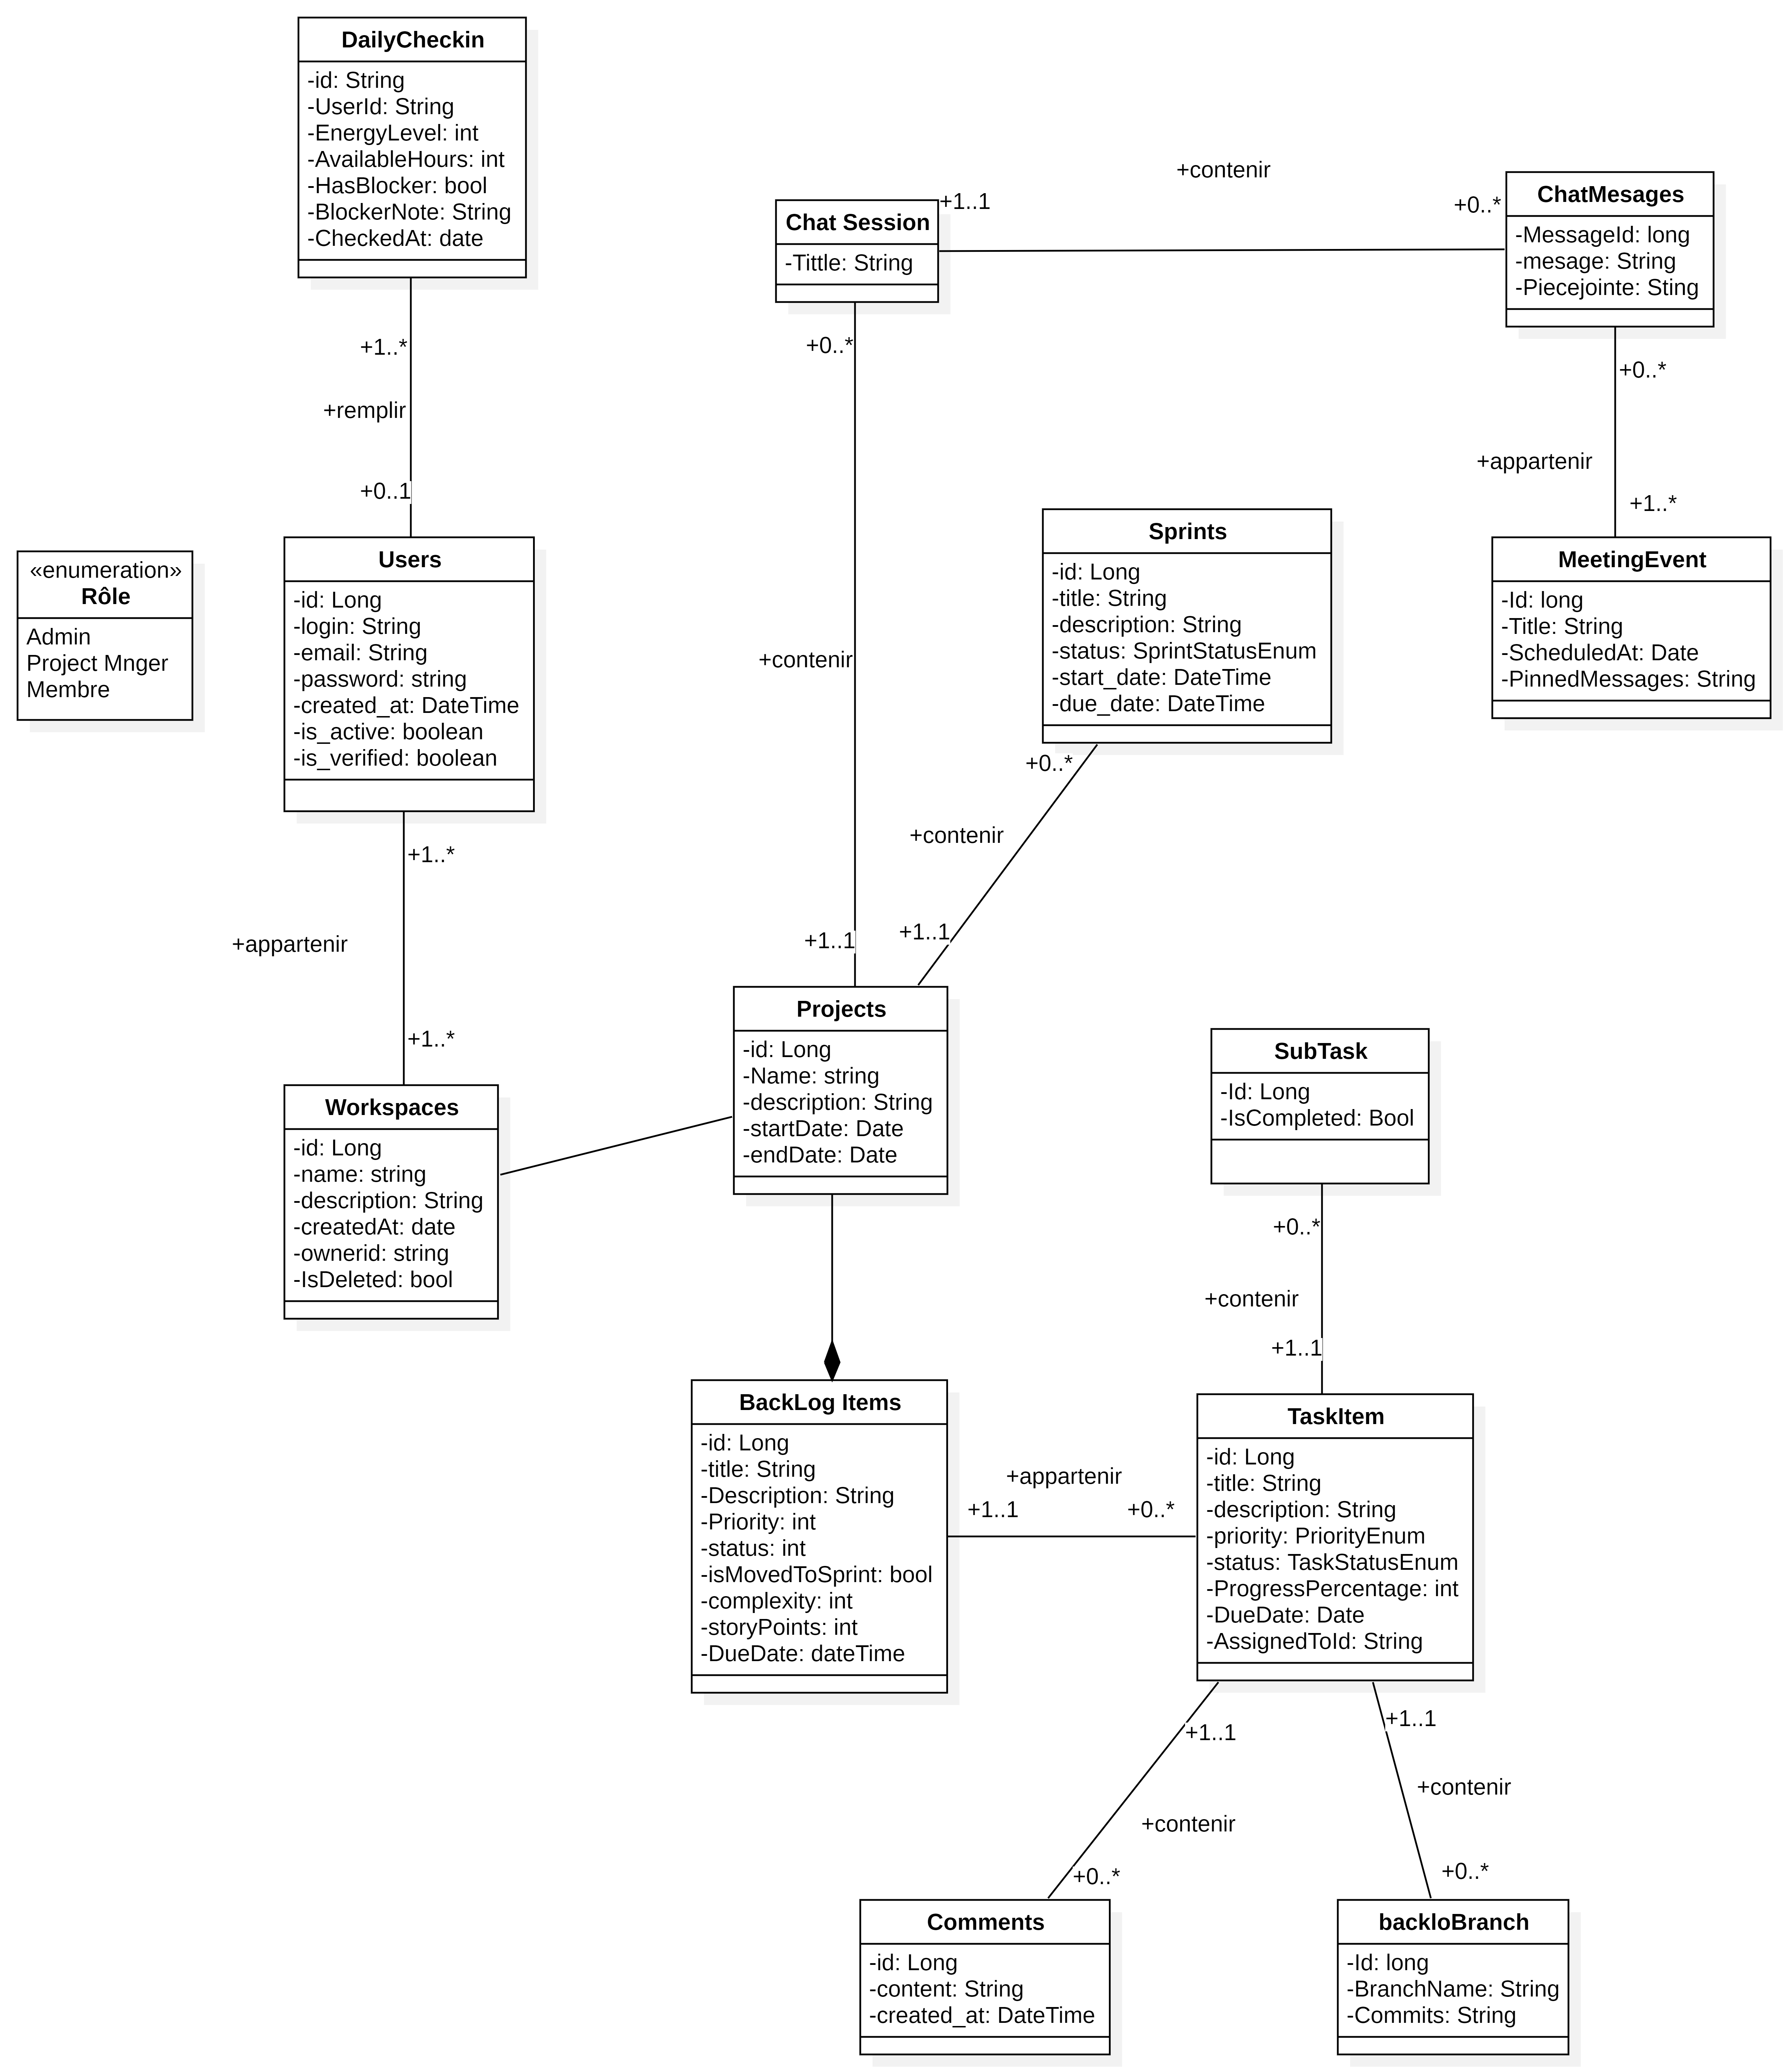
\includegraphics[width=1\linewidth]{ClassDiagram1.png}
  \caption{Diagramme de classes général de l'application Planora}
  \label{fig:DiagrammeClasseGeneral}
\end{figure}

\subsection{Gestion de l'authentification et des utilisateurs}

\subsubsection{Diagramme de séquence}

Au niveau de la page de connexion, l'utilisateur saisit son adresse email et son mot de passe afin d'accéder à l'application Planora. Le système vérifie les informations d'identification, puis génère un jeton d'authentification si les données saisies sont correctes.\\
Après authentification, l'utilisateur est redirigé vers le tableau de bord et accède aux fonctionnalités autorisées selon son rôle : Administrateur, ProjectManager ou Member.\\
L'administrateur peut également gérer les comptes utilisateurs, modifier leurs informations, attribuer des rôles, activer ou désactiver un compte.\\
La figure \ref{fig:GestionAuthentificationSequence} illustre le diagramme de séquence de la gestion de l'authentification et des utilisateurs.

\begin{figure}[H]
  \centering
   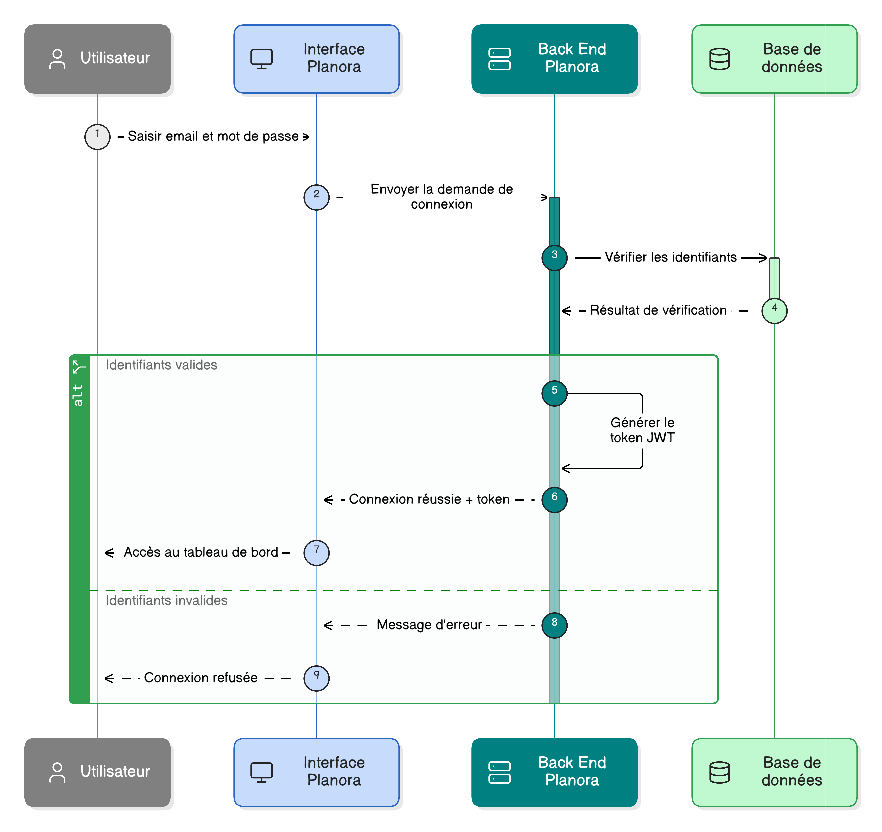
\includegraphics[width=0.7\linewidth]{Authentification.png}
  \caption{Diagramme de séquence de la gestion de l'authentification et des utilisateurs}
  \label{fig:GestionAuthentificationSequence}
\end{figure}

\subsection{Gestion des espaces de travail et des projets}

\subsubsection{Diagramme de séquence}

L'administrateur crée un espace de travail en renseignant les informations nécessaires, telles que le nom et la description. Une fois l'espace créé, il peut inviter des membres à le rejoindre. Les utilisateurs invités reçoivent une invitation qu'ils peuvent accepter ou refuser.\\
Après l'organisation de l'espace de travail, le ProjectManager peut créer un projet, définir ses informations principales, affecter des membres et suivre son avancement. Les membres ajoutés au projet peuvent ensuite accéder aux fonctionnalités qui leur sont autorisées.\\
La figure \ref{fig:GestionWorkspaceProjetSequence} illustre le diagramme de séquence de la gestion des espaces de travail et des projets.

\begin{figure}[H]
  \centering
   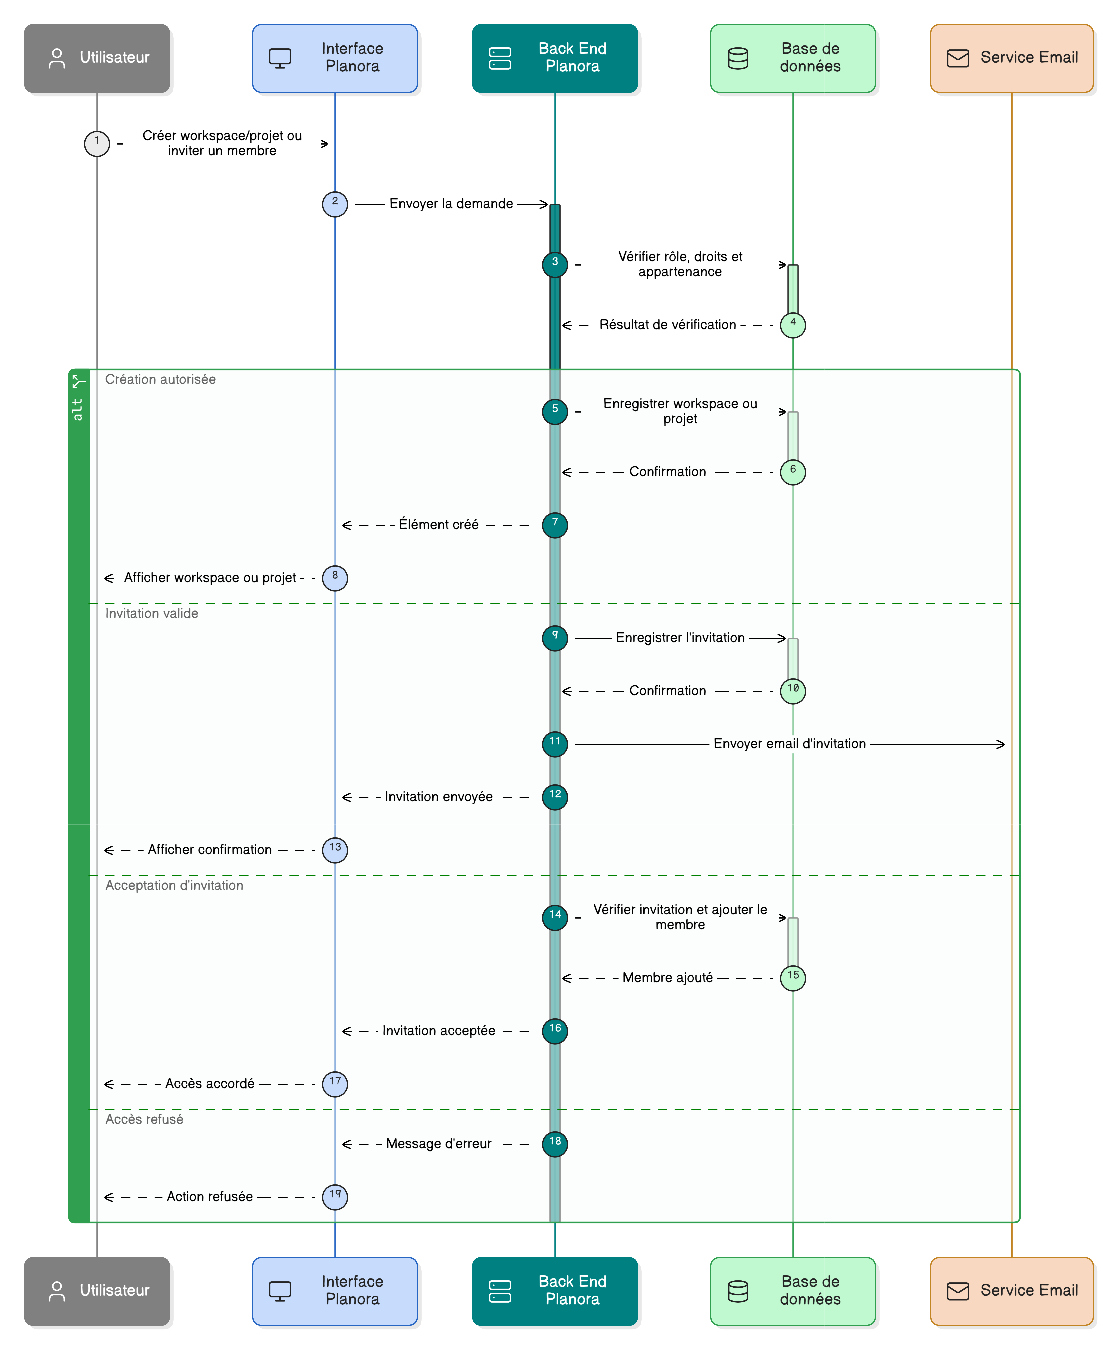
\includegraphics[width=0.7\linewidth]{Project Espace Travail.png}
  \caption{Diagramme de séquence de la gestion des espaces de travail et des projets}
  \label{fig:GestionWorkspaceProjetSequence}
\end{figure}

\subsection{Gestion du backlog, des tâches et des sprints}

\subsubsection{Diagramme de séquence}

Le ProjectManager ou un membre autorisé accède au backlog d'un projet afin de créer de nouveaux éléments. Chaque élément du backlog peut contenir un titre, une description, une priorité, une complexité, des story points, une date d'échéance et un membre assigné.\\
Les éléments du backlog peuvent être associés à un sprint afin d'organiser le travail selon une approche agile. Les membres peuvent ensuite suivre l'état d'avancement des tâches, ajouter des commentaires et mettre à jour les informations nécessaires.\\
La figure \ref{fig:GestionBacklogSprintSequence} illustre le diagramme de séquence de la gestion du backlog, des tâches et des sprints.

\begin{figure}[H]
  \centering
   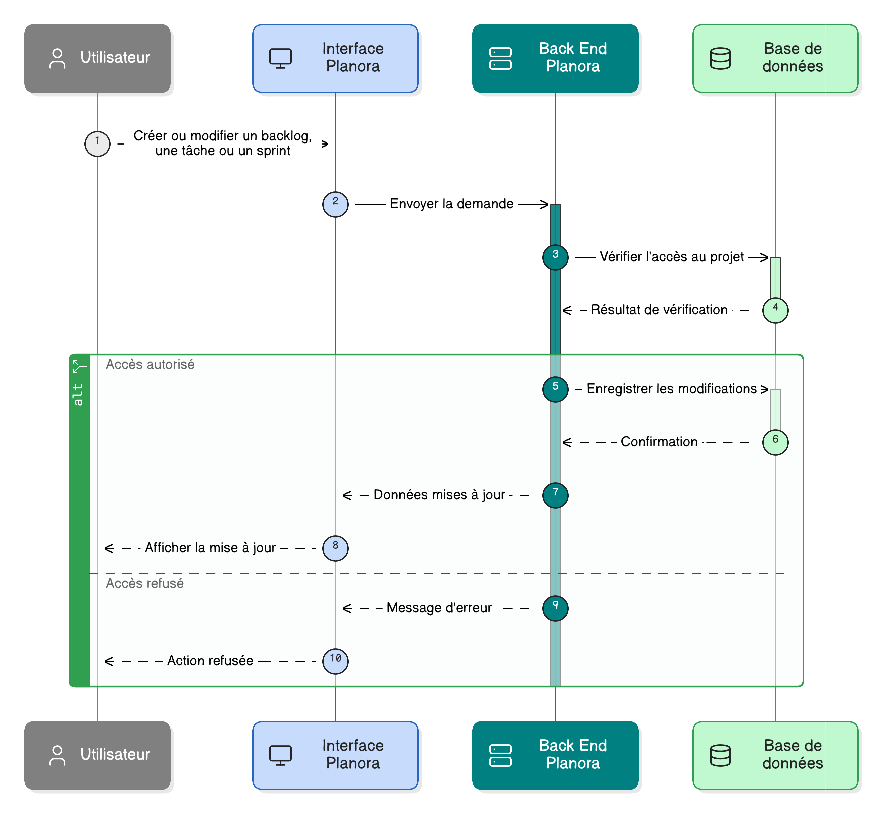
\includegraphics[width=0.7\linewidth]{Backlog And Stuff.png}
  \caption{Diagramme de séquence de la gestion du backlog, des tâches et des sprints}
  \label{fig:GestionBacklogSprintSequence}
\end{figure}

\subsection{Gestion de la collaboration et des réunions}

\subsubsection{Diagramme de séquence}

Les membres d'un projet peuvent communiquer à travers un espace de messagerie intégré. Lorsqu'un utilisateur envoie un message, celui-ci est enregistré et rattaché à une session de discussion liée au projet. Les autres membres concernés peuvent consulter les messages et suivre les échanges.\\
La plateforme permet également de planifier des réunions à travers un calendrier. L'utilisateur renseigne les informations de la réunion, telles que le titre, la date, l'heure et les membres concernés. Le système enregistre ensuite l'événement et l'affiche dans le calendrier du projet.\\
La figure \ref{fig:GestionCollaborationSequence} illustre le diagramme de séquence de la gestion de la collaboration et des réunions.

\begin{figure}[H]
  \centering
   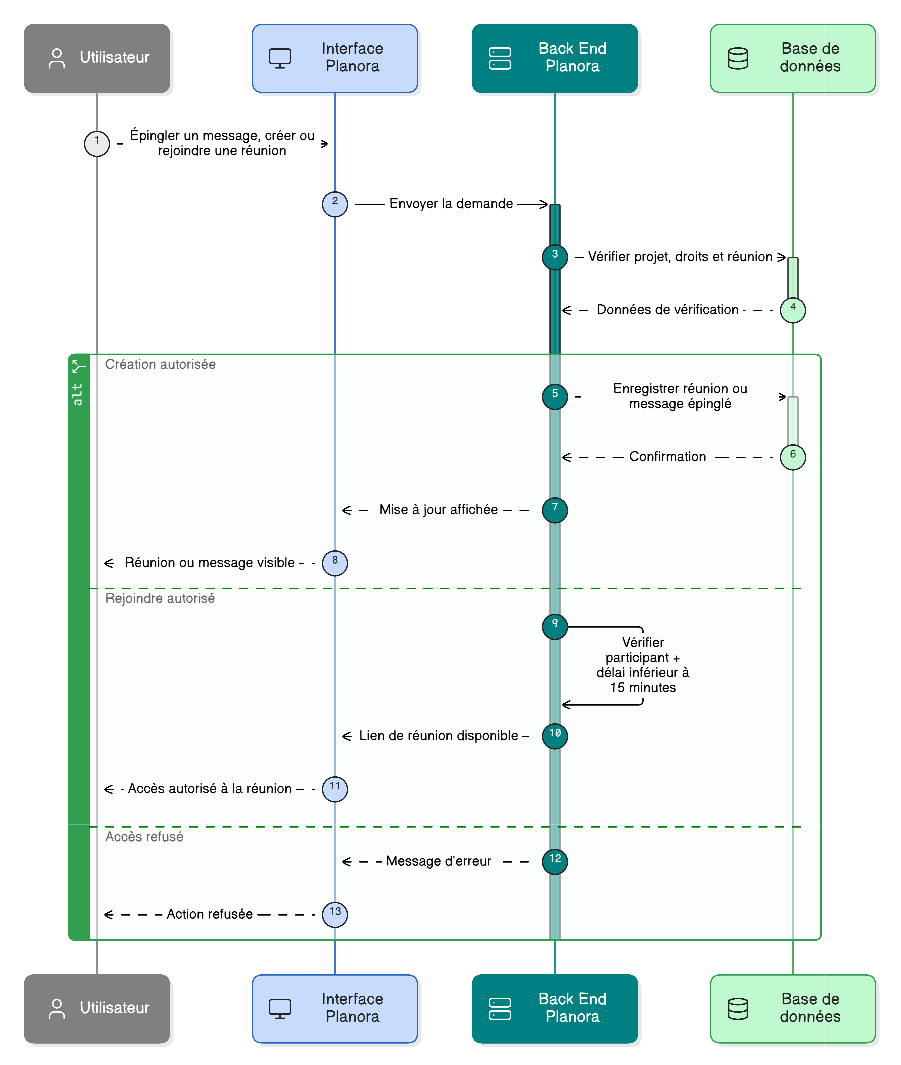
\includegraphics[width=0.7\linewidth]{Collaboration Reunion.png}
  \caption{Diagramme de séquence de la gestion de la collaboration et des réunions}
  \label{fig:GestionCollaborationSequence}
\end{figure}

\subsection{Suivi de la santé de l'équipe par intelligence artificielle}

\subsubsection{Diagramme de séquence}

Le suivi de la santé de l'équipe repose sur un module d'intelligence artificielle permettant d'analyser les messages échangés entre les membres d'un projet. Lorsqu'un utilisateur accède à la page dédiée, le système récupère les messages récents et les transmet au service d'analyse.\\
Le modèle d'intelligence artificielle classe les messages selon plusieurs sentiments, notamment positif, neutre, stressé ou frustré. À partir de ces résultats, le système calcule un score global, génère une distribution des sentiments et affiche des alertes lorsque des signes de stress ou de frustration sont détectés.\\
La figure \ref{fig:TeamHealthSequence} illustre le diagramme de séquence du suivi de la santé de l'équipe par intelligence artificielle.

\begin{figure}[H]
  \centering
   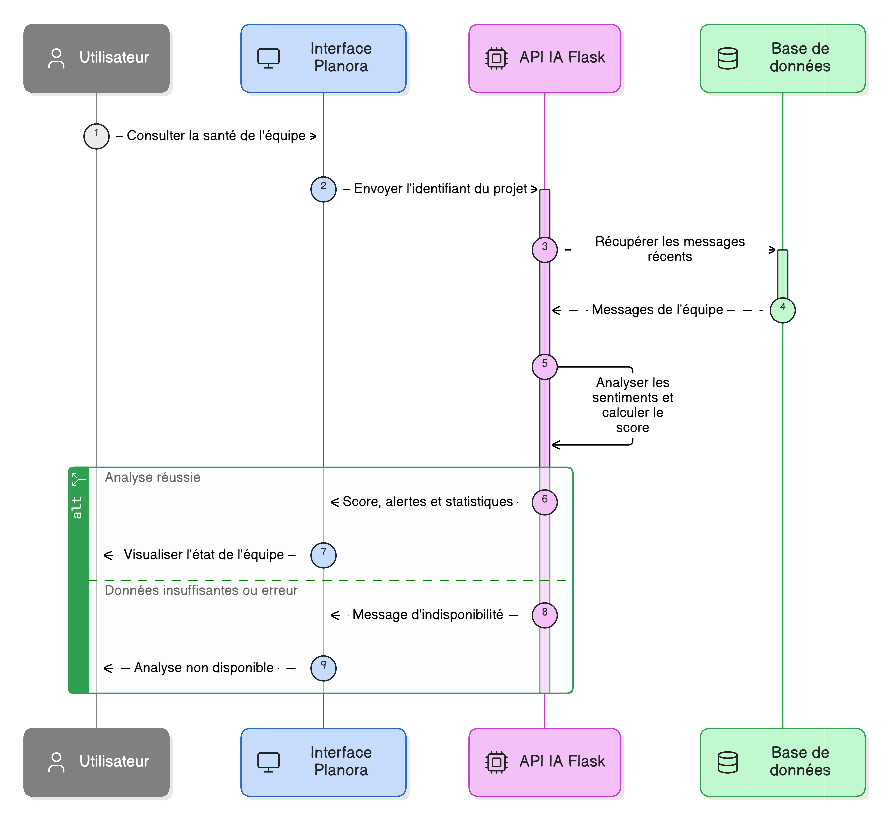
\includegraphics[width=1\linewidth]{Sante equipe suivie.png}
  \caption{Diagramme de séquence du suivi de la santé de l'équipe par intelligence artificielle}
  \label{fig:TeamHealthSequence}
\end{figure}

\subsubsection{Diagramme de séquence du chatbot IA}

Le chatbot intelligent permet aux utilisateurs d’interagir directement avec un assistant intégré dans la plateforme. Lorsqu’un utilisateur ouvre la fenêtre de chat, le système initialise la conversation et permet l’envoi de messages texte, emojis ou fichiers.

Le chatbot analyse les requêtes des utilisateurs et peut répondre à des questions, fournir des explications ou analyser le contenu d’un fichier ou d’une image envoyée. Les messages sont transmis au modèle d’intelligence artificielle, qui génère une réponse adaptée en fonction du contexte de la conversation.\\
La figure \ref{fig:ChatbotAISequence} illustre le diagramme de séquence du chatbot IA.

\begin{figure}[H]
  \centering
  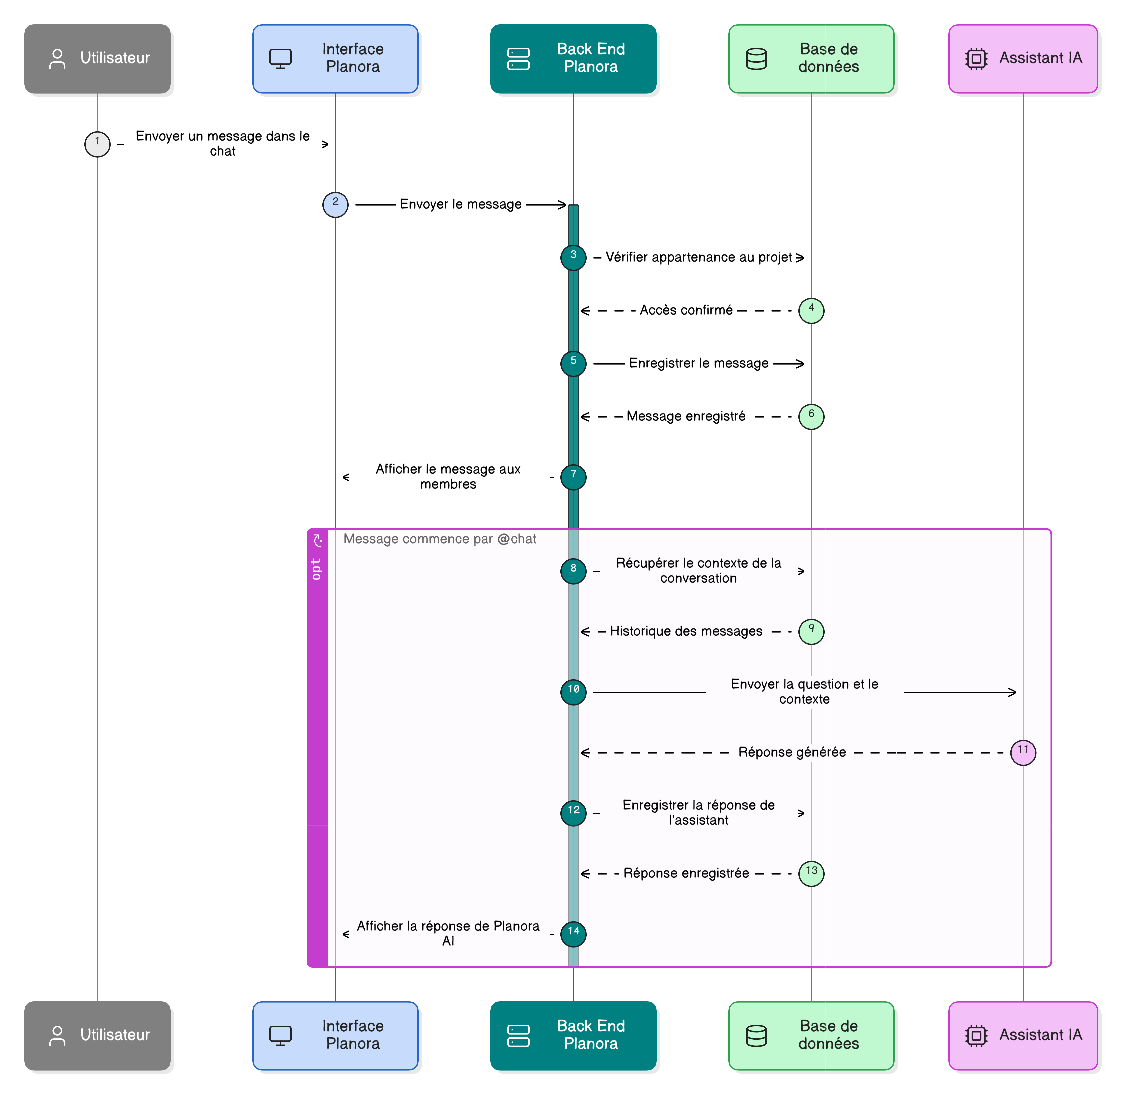
\includegraphics[width=1\linewidth]{Chat.png}
  \caption{Diagramme de séquence du chatbot IA}
  \label{fig:ChatbotAISequence}
\end{figure}
\section*{Conclusion}

Dans ce chapitre, nous avons présenté la conception détaillée de l'application Planora à travers les principaux diagrammes de séquence décrivant les interactions entre les acteurs et le système. Nous avons également présenté le diagramme de classes général afin de modéliser la structure globale de l'application et les relations entre ses principales entités.

%%%%% Conclusion
\chapter{Réalisation}

\section*{Introduction}
Dans ce chapitre, nous présenterons les outils de développement utilisés, ainsi que l'architecture technique adoptée pour le processus de développement. Ensuite, nous détaillerons les incréments réalisés à chaque sprint, illustrant les différentes fonctionnalités du projet.

\section{Environnement de développement}
\subsection{SQL Server Management Studio}
SQL Server Management Studio (\ac{SSMS}), développé par Microsoft en 2005, est un environnement de gestion intégré pour les bases de données SQL Server. Il offre une interface graphique complète pour la gestion, le développement et l'administration des bases de données SQL Server, facilitant ainsi les tâches telles que la création de requêtes, la gestion des objets de base de données et la surveillance des performances. \cite{SSMS}

\begin{figure}[H]
  \centering
  
\includegraphics[width=0.14\columnwidth]{SSMS_Logo.jpg}
  \caption{Logo de SQL Server Management Studio}
  \label{fig:SSMS}
\end{figure}

\subsection{Visual Studio}
Visual Studio (\ac{VS}), développé par Microsoft en 2005, est un environnement de développement intégré (IDE) puissant. Il propose une suite complète de fonctionnalités concentrées pour faciliter la création, la modification et le débogage des applications .NET. \cite{VisualStudio}

\begin{figure}[H]
  \centering
  
\includegraphics[width=0.14\columnwidth]{Visual_Studio_Icon_2026.svg.png}
  \caption{Logo de Visual Studio}
  \label{fig:VisualStudio}
\end{figure}

\subsection{Visual Studio Code}
Visual Studio Code (\ac{VSCode}), développé par Microsoft en 2015, est un éditeur de code qui peut être étendu avec des extensions pour le transformer en un environnement de développement intégré (IDE) complet. \cite{VsCode}

\begin{figure}[H]
  \centering
  
\includegraphics[width=0.14\columnwidth]{Visual_Studio_Code_1.35_icon.svg.png}
  \caption{Logo de Visual Studio Code}
  \label{fig:VsCode}
\end{figure}

\subsection{Swagger}
Swagger est un ensemble d'outils open source développé par SmartBear Software,
permettant de concevoir, documenter et tester les APIs RESTful de manière
standardisée et interactive \cite{swagger}.

\begin{figure}[H]
  \centering
  
\includegraphics[width=0.15\columnwidth]{images.png}
  \caption{Logo de Swagger}
  \label{fig:Swagger}
\end{figure}

\section{Environnement logiciel}
\subsection{Microsoft SQL Server}
SQL Server, initialement lancé en 1989, est un système de gestion de bases de données relationnelles développé par Microsoft. Il offre une plateforme complète pour la gestion et l'analyse des données, avec des fonctionnalités avancées de sécurité, de performance et de disponibilité. \cite{SQLServer}

\begin{figure}[H]
  \centering
  
\includegraphics[width=0.2\columnwidth]{Microsoft_SQL_Server_2025_icon.svg.png}
  \caption{Logo de Microsoft SQL Server}
  \label{fig:SQLServer}
\end{figure}

\subsection{Dotnet}
Dotnet (\ac{DOTNET}), développé par Microsoft et lancé en 2002, est une plateforme de développement logiciel qui permet de créer et d'exécuter des applications sur plusieurs systèmes d'exploitation. Elle offre une grande variété de langages de programmation et d'outils pour faciliter le développement d'applications modernes.\cite{Dotnet}

\begin{figure}[H]
  \centering
  
\includegraphics[width=0.14\columnwidth]{dotnet-logo.png}
  \caption{Logo de Dotnet}
  \label{fig:Dotnet}
\end{figure}

\subsection{LaTeX}
LaTeX, développé par Leslie Lamport en 1985, est un système de composition de documents qui permet de créer des documents de haute qualité typographique. Il est largement utilisé dans les domaines académiques et scientifiques pour la rédaction d'articles, de rapports et de thèses.\cite{Latex}

\begin{figure}[H]
  \centering
  
\includegraphics[width=0.18\columnwidth]{latex-logo.png}
  \caption{Logo de LaTeX}
  \label{fig:Latex}
\end{figure}

\section{Pilotage du cycle de vie de développement avec Scrum}
Dans cette section, nous mettrons en lumière l'application de la méthode Scrum pour piloter le projet. Nous présenterons les membres de l'équipe ainsi que leurs rôles respectifs, puis nous examinerons le backlog du produit.
\subsection{Équipe Scrum et rôles}
La création d'une équipe Scrum solide est une étape essentielle pour la réussite d'un projet.\\
Les membres de l'équipe Scrum ainsi que leurs rôles sont illustrés dans la figure \ref{fig:scrum_team} ci-dessous :

\begin{figure}[H]
  \centering
  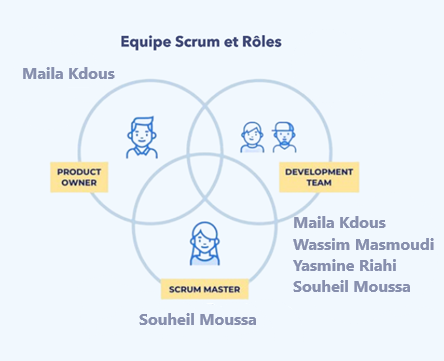
\includegraphics[width=0.7\columnwidth]{equipeScrum.png}
  \caption{Équipe Scrum et rôles}
  \label{fig:scrum_team}
\end{figure}

\section{Architecture technique}
\subsection{Architecture générale}
L'application web conçue sera déployée selon une architecture à 3 niveaux (3-Tiers). \\
Cette architecture est représentée par la figure \ref{fig:ArchitectureGenerale} :
\begin{figure}[H]
  \centering
  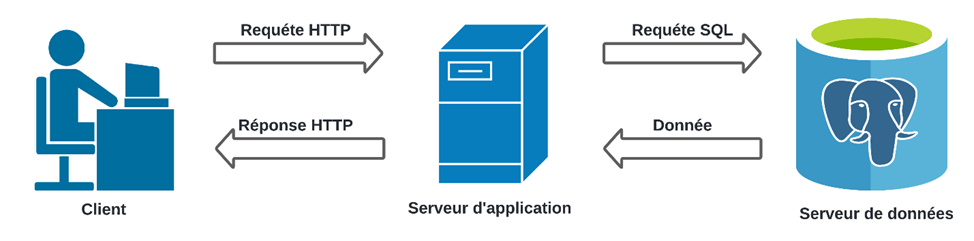
\includegraphics[width=1\linewidth]{ArchitectureGenerale.png}
  \caption{Architecture générale}
  \label{fig:ArchitectureGenerale}
\end{figure}

\subsection{Architecture de l'environnement}
Dans cette section, nous explorerons l'architecture technique de l'application, en décrivant ses différentes composantes techniques, à savoir, le Back End et le Front End.
\subsubsection{Architecture du Back End}
Le Back End de l'application Planora est développé avec ASP.NET Core et repose sur une architecture basé sur la "Clean Architecture". Cette organisation permet de séparer les responsabilités entre la présentation des services API, la logique applicative, la logique métier et l'accès aux données. Elle facilite également la maintenance, l'évolution et le test de l'application.

L'architecture Back End est composée principalement des couches suivantes :
\begin{itemize}
  \item[$\bullet$] \textbf{Couche \ac{API} "Planora"} : Cette couche représente le point d'entrée de l'application côté serveur. Elle contient les contrôleurs \ac{API} REST qui reçoivent les requêtes HTTP provenant du Front End, valident l'accès de l'utilisateur, appellent les services nécessaires et retournent les réponses sous forme d'objets \ac{JSON}. Elle contient également la configuration générale de l'application, le middleware de gestion des erreurs et le hub \ac{SignalR} utilisé pour la communication en temps réel.

  \item[$\bullet$] \textbf{Couche Application "Planora.Application"} : Cette couche regroupe les contrats et les objets de transfert de données utilisés par l'application. Elle contient les interfaces des services, les DTOs, les validateurs et les profils de mapping. Son rôle est de définir les opérations disponibles sans dépendre directement de leur implémentation technique.

  \item[$\bullet$] \textbf{Couche Domaine "Planora.Domain"} : Cette couche contient les entités principales du système, telles que ApplicationUser, Workspace, Project, BacklogItem, Sprint, TaskItem, Comment et ChatMessage. Elle représente le cœur métier de l'application et définit la structure des données manipulées par Planora.

  \item[$\bullet$] \textbf{Couche Infrastructure "Planora.Infrastructure"} : Cette couche contient les implémentations concrètes des services, les repositories, le contexte de base de données, les configurations Entity Framework Core, les migrations et les services techniques comme l'authentification par \ac{JWT}, l'envoi d'emails et l'intégration avec la base de données. Elle assure la communication avec SQL Server et réalise les traitements nécessaires à la persistance des données.

  \item[$\bullet$] \textbf{Module IA "planora-ai"} : Ce module est développé en Python avec Flask. Il expose une API dédiée à l'analyse des messages échangés entre les membres d'un projet. Le modèle d'intelligence artificielle classe les messages selon leur sentiment et renvoie les résultats au Back End ou au Front End afin d'afficher les indicateurs de santé de l'équipe.
\end{itemize}

Ainsi, cette architecture permet de garantir une séparation claire entre les différentes responsabilités du système.

\subsubsection{Architecture du Front End}
L'architecture utilisée dans la partie Front End est une architecture basée sur les composants, comprenant les différentes parties suivantes :
\begin{itemize}
  \item[$\bullet$] \textbf{Composants}: Ce sont les blocs de construction de l'interface utilisateur (UI). Chaque composant représente une partie de l'UI et est responsable de sa propre logique afin de réaliser une fonction spécifique.
  \item[$\bullet$] \textbf{Services}: Ils sont utilisés pour encapsuler la logique métier qui n'appartient pas spécifiquement à un composant particulier, telle que gérer les appels \ac{API} REST, et les fonctionnalités transversales à plusieurs composants.
  \item[$\bullet$] \textbf{Modules}: Ce sont des regroupements logiques de composants, de services et d'autres fonctionnalités de l'application afin de permettre une organisation du code de manière modulaire.
\end{itemize}
Il convient de noter que cette architecture favorise la création d'applications modulaires grâce à des composants interchangeables et réutilisables.

\subsection{Protocole de sécurité}
Le protocole de sécurité est un ensemble de règles et de procédures destiné à protéger
les données et les systèmes informatiques contre les accès non autorisés, les attaques et
les dommages.
\subsubsection{Protocole de sécurité LDAP}
LDAP est un protocole utilisé pour accéder et gérer les services d'annuaire distribué,
permettant de rechercher et de modifier des informations dans un annuaire de réseau,
souvent utilisé pour l'authentification et la gestion des utilisateurs.
\begin{figure}[H]
  \centering
  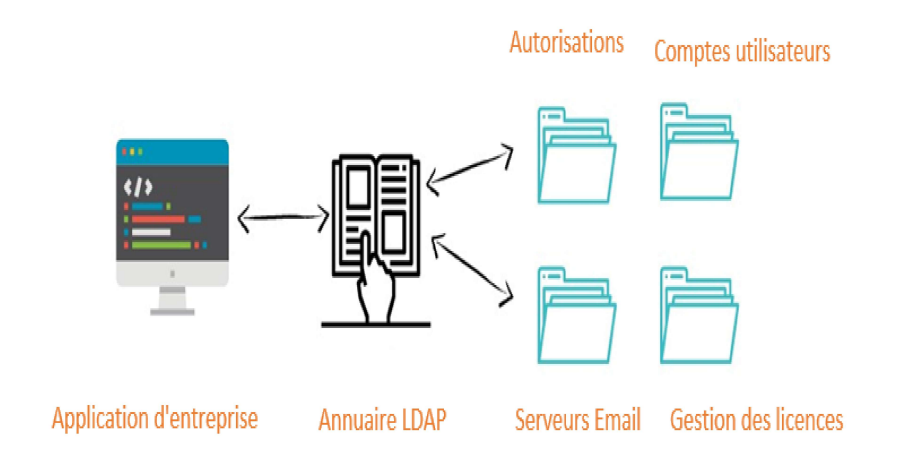
\includegraphics[width=1\linewidth]{i12.png}
  \caption{Protocole de sécurité LDAP}
  \label{fig:Protocole de sécurité LDAP}
\end{figure}

\subsection{Backlog du produit}
Dans cette section, nous présenterons les différentes fonctionnalités du produit et décrirons les scénarios d'utilisation associés à travers des stories utilisateur. Cette approche permettra de formaliser efficacement les besoins des utilisateurs et de prioriser le travail de développement.\\
Ci-dessous, nous détaillons la signification des différents termes utilisés dans le backlog produit :
\begin{itemize}
  \item \textbf{ID} : Identifiant unique de chaque fonctionnalité.
  \item \textbf{Fonctionnalité} : Une caractéristique particulière proposée par l'application.
  \item \textbf{User Story} : Une fonctionnalité que l'utilisateur final souhaite accomplir avec le système applicatif.
  \item \textbf{Priorité} : Niveau d'importance ou d'urgence attribué à une User Story.
\end{itemize}
Le tableau \ref{tab:backlog-produit} présente le backlog du produit ainsi que la priorisation des fonctionnalités.

\subsubsection{Légende des priorités}
\begin{table}[H]
  \centering
  \caption{Légende des priorités du backlog}
  \label{tab:legende-priorites-backlog}
  \renewcommand{\arraystretch}{1.2}
  \begin{tabular}{|p{3cm}|p{10cm}|}
    \hline
    \textbf{Priorité}                           & \textbf{Signification}                                                          \\
    \hline
    \cellcolor{niveauCritique}\textbf{Critique} & À réaliser en premier car l'élément conditionne plusieurs autres tâches.        \\
    \hline
    \cellcolor{niveauEleve}\textbf{Élevé}       & À traiter rapidement car l'impact fonctionnel ou technique est important.       \\
    \hline
    \cellcolor{niveauMoyen}\textbf{Moyen}       & À planifier après les fondations principales, avec une dépendance plus limitée. \\
    \hline
    \cellcolor{niveauFaible}\textbf{Faible}     & À intégrer en dernier, une fois le socle applicatif stabilisé.                  \\
    \hline
  \end{tabular}
\end{table}

\subsubsection{Backlog du produit}
\small
\renewcommand{\arraystretch}{1.25}
\enlargethispage{3\baselineskip}
\begin{longtable}{|p{0.8cm}|p{3.7cm}|p{5.3cm}|p{1.8cm}|p{3.8cm}|}
  \caption{Backlog du produit et priorisation des tâches}\label{tab:backlog-produit}                                                                                                                                                                                                                                                                                \\
  \hline
  \textbf{ID} & \textbf{Fonctionnalité}                   & \textbf{User Story}                                                                                                                                          & \textbf{Priorité}                           & \textbf{Remarques}                                                                         \\
  \hline
  \endfirsthead

  \hline
  \textbf{ID} & \textbf{Fonctionnalité}                   & \textbf{User Story}                                                                                                                                          & \textbf{Priorité}                           & \textbf{Remarques}                                                                         \\
  \hline
  \endhead

  \hline
  \endfoot

  \hline
  \endlastfoot

  1           & Authentification et inscription           & En tant qu'utilisateur, je veux créer un compte et m'authentifier afin d'accéder à l'application Planora de manière sécurisée.                               & \cellcolor{niveauCritique}\textbf{Critique} & Fonction de base nécessaire pour accéder aux autres modules.                               \\
  \hline

  2           & Gestion des rôles et des utilisateurs     & En tant qu'administrateur, je veux gérer les comptes utilisateurs, leurs rôles et leur état d'activation afin de contrôler les accès à la plateforme.        & \cellcolor{niveauCritique}\textbf{Critique} & Conditionne la sécurité et la séparation des droits entre Admin, ProjectManager et Member. \\
  \hline

  3           & Gestion des espaces de travail            & En tant qu'administrateur, je veux créer des espaces de travail et inviter des membres afin d'organiser les équipes dans des environnements séparés.         & \cellcolor{niveauCritique}\textbf{Critique} & Structure principale de l'organisation des projets.                                        \\
  \hline

  4           & Gestion des projets                       & En tant que ProjectManager, je veux créer et gérer des projets afin de planifier le travail et suivre l'avancement de l'équipe.                              & \cellcolor{niveauCritique}\textbf{Critique} & Dépend de la gestion des espaces de travail et des membres.                                \\
  \hline

  5           & Gestion du backlog                        & En tant que ProjectManager, je veux créer, modifier, prioriser et assigner les éléments du backlog afin d'organiser les besoins du projet.                   & \cellcolor{niveauEleve}\textbf{Élevé}       & Module central pour la gestion agile du projet.                                            \\
  \hline

  6           & Gestion des tâches et sous-tâches         & En tant que membre de projet, je veux consulter, mettre à jour et suivre mes tâches afin de contribuer efficacement à l'avancement du projet.                & \cellcolor{niveauEleve}\textbf{Élevé}       & Complète la gestion du backlog et permet le suivi opérationnel.                            \\
  \hline

  7           & Gestion des sprints                       & En tant que ProjectManager, je veux créer des sprints et y associer des éléments du backlog afin de planifier le travail par itérations.                     & \cellcolor{niveauEleve}\textbf{Élevé}       & Nécessaire pour organiser le projet selon une approche agile.                              \\
  \hline

  8           & Tableau de bord                           & En tant qu'utilisateur autorisé, je veux consulter des statistiques et indicateurs afin de suivre l'avancement des projets et des espaces de travail.        & \cellcolor{niveauEleve}\textbf{Élevé}       & Permet une vision synthétique de l'état des projets.                                       \\
  \hline

  9           & Messagerie de projet                      & En tant que membre de projet, je veux échanger des messages avec les autres membres afin de faciliter la collaboration.                                      & \cellcolor{niveauMoyen}\textbf{Moyen}       & Supporte la communication interne et alimente le module d'analyse de santé.                \\
  \hline

  10          & Gestion des réunions et calendrier        & En tant que membre de projet, je veux planifier et consulter les réunions afin de mieux organiser les échanges de l'équipe.                                  & \cellcolor{niveauMoyen}\textbf{Moyen}       & Complète les fonctionnalités collaboratives du projet.                                     \\
  \hline

  11          & Commentaires et pièces jointes du backlog & En tant que membre de projet, je veux ajouter des commentaires, liens et pièces jointes aux éléments du backlog afin de centraliser les informations utiles. & \cellcolor{niveauMoyen}\textbf{Moyen}       & Enrichit le suivi détaillé des éléments du backlog.                                        \\
  \hline

  12          & Suivi de la santé de l'équipe par IA      & En tant que ProjectManager, je veux analyser les messages de l'équipe afin de détecter le stress, la frustration et l'ambiance générale du projet.           & \cellcolor{niveauMoyen}\textbf{Moyen}       & Dépend de la messagerie et du module IA Python Flask.                                      \\
  \hline

  13          & Notifications par email                   & En tant qu'utilisateur, je veux recevoir des notifications importantes afin d'être informé des invitations et des affectations de tâches.                    & \cellcolor{niveauFaible}\textbf{Faible}     & Améliore l'expérience utilisateur sans bloquer les modules principaux.                     \\
  \hline

  14          & Check-in quotidien                        & En tant que membre de projet, je veux renseigner mon niveau d'énergie, mes disponibilités et mes blocages afin d'aider au suivi de l'équipe.                 & \cellcolor{niveauFaible}\textbf{Faible}     & Fonction complémentaire au suivi de la santé de l'équipe.                                  \\
  \hline
\end{longtable}

\normalsize

\section{Sprints de réalisation}

Dans cette section, nous présentons les incréments réalisés sprint par sprint, en détaillant le backlog associé à chaque itération ainsi que les interfaces livrées. Le découpage respecte les dépendances fonctionnelles du projet : d'abord l'authentification, la gestion des utilisateurs, des espaces de travail et des projets, ensuite la gestion agile et le tableau de bord, et enfin la collaboration, les réunions et le module d'intelligence artificielle.

%------------------------------------------------------------
\subsection{Sprint 1 - Authentification, gestion des utilisateurs, des espaces de travail et des projets}
%------------------------------------------------------------
\subsubsection{Backlog du sprint}
Le tableau \ref{tab:backlog-sprint1} illustre le backlog du Sprint 1.

\enlargethispage{2\baselineskip}
\begin{longtable}{|p{5.8cm}|p{1.3cm}|p{7.2cm}|}
  \caption{Backlog du Sprint 1 : Authentification, gestion des utilisateurs, des espaces de travail et des projets}\label{tab:backlog-sprint1} \\
  \hline
  \textbf{User Story} & \textbf{ID} & \textbf{Tâches} \\
  \hline
  \endfirsthead
  \hline
  \textbf{User Story} & \textbf{ID} & \textbf{Tâches} \\
  \hline
  \endhead
  \hline
  \endfoot
  \hline
  \endlastfoot

  En tant qu'utilisateur, je veux créer un compte afin d'accéder à l'application Planora.
                      & 1.1         & \textbullet~Créer l'interface d'inscription. \\
  \cline{2-3}
                      & 1.2         & \textbullet~Implémenter l'\ac{API} d'inscription côté Back End. \\
  \cline{2-3}
                      & 1.3         & \textbullet~Valider les informations saisies par l'utilisateur. \\
  \hline

  En tant qu'utilisateur, je veux m'authentifier afin d'accéder aux fonctionnalités selon mon rôle.
                      & 1.4         & \textbullet~Créer l'interface de connexion. \\
  \cline{2-3}
                      & 1.5         & \textbullet~Mettre en place l'authentification par \ac{JWT}. \\
  \cline{2-3}
                      & 1.6         & \textbullet~Protéger les routes du Front End avec un guard d'authentification. \\
  \hline

  En tant qu'administrateur, je veux gérer les utilisateurs et leurs rôles afin de contrôler les accès à la plateforme.
                      & 1.7         & \textbullet~Créer les rôles Admin, ProjectManager et Member. \\
  \cline{2-3}
                      & 1.8         & \textbullet~Développer la gestion des utilisateurs côté Back End. \\
  \cline{2-3}
                      & 1.9         & \textbullet~Permettre l'activation, la désactivation et l'attribution des rôles. \\
  \hline

  En tant qu'administrateur, je veux créer des espaces de travail afin d'organiser les équipes et les projets.
                      & 1.10        & \textbullet~Créer l'entité Workspace et ses relations. \\
  \cline{2-3}
                      & 1.11        & \textbullet~Développer les API de création, consultation et suppression des espaces de travail. \\
  \cline{2-3}
                      & 1.12        & \textbullet~Créer les interfaces de gestion des espaces de travail. \\
  \hline

  En tant qu'administrateur ou ProjectManager, je veux inviter des membres afin de constituer une équipe de travail.
                      & 1.13        & \textbullet~Mettre en place le système d'invitations aux espaces de travail. \\
  \cline{2-3}
                      & 1.14        & \textbullet~Permettre l'acceptation et le refus des invitations. \\
  \cline{2-3}
                      & 1.15        & \textbullet~Afficher la liste des membres d'un espace de travail. \\
  \hline

  En tant que ProjectManager, je veux créer et gérer des projets afin de suivre leur avancement.
                      & 1.16        & \textbullet~Créer l'entité Project et ses relations avec Workspace et ApplicationUser. \\
  \cline{2-3}
                      & 1.17        & \textbullet~Développer les API de création, modification et consultation des projets. \\
  \cline{2-3}
                      & 1.18        & \textbullet~Créer les interfaces de liste et de détail des projets. \\
  \hline
\end{longtable}


\subsubsection{Interfaces livrables}

La figure \ref{fig:sprint1-login} illustre l'interface de connexion permettant à l'utilisateur de s'authentifier avec son adresse email et son mot de passe.

\begin{figure}[H]
  \centering
  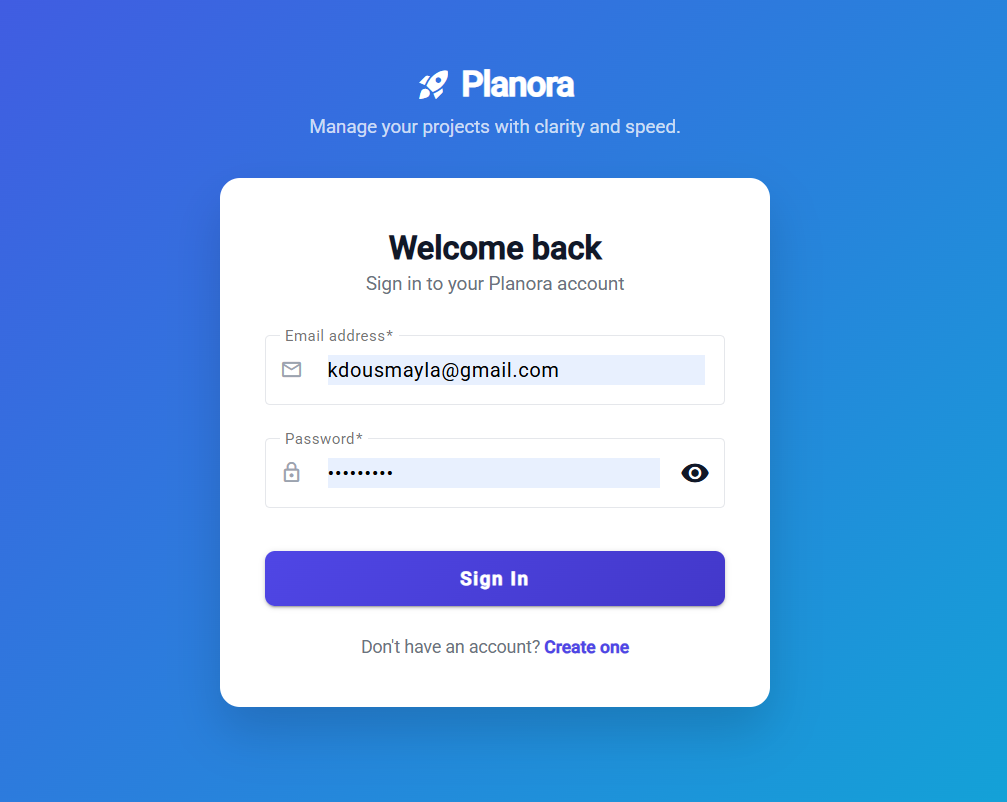
\includegraphics[width=0.6\columnwidth]{i1.png}
  \caption{Sprint 1 - Interface de connexion}
  \label{fig:sprint1-login}
\end{figure}

La figure \ref{fig:sprint1-register} présente l'interface d'inscription permettant à un nouvel utilisateur de créer son compte.

\begin{figure}[H]
  \centering
  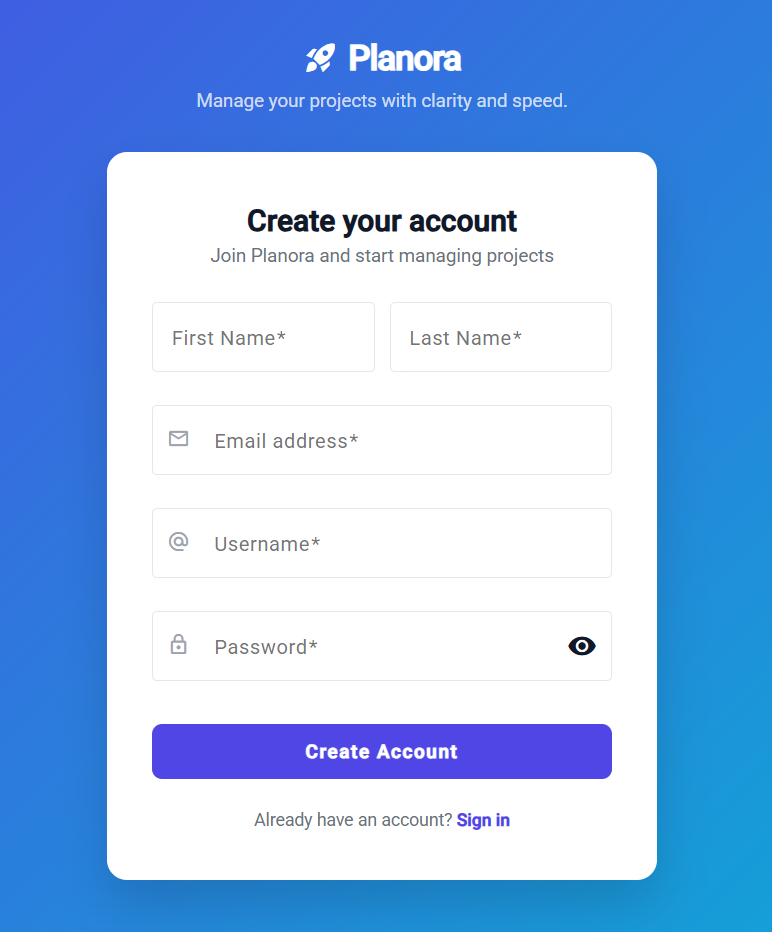
\includegraphics[width=0.4\columnwidth]{i2.png}
  \caption{Sprint 1 - Interface d'inscription}
  \label{fig:sprint1-register}
\end{figure}

La figure \ref{fig:sprint1-users} illustre l'interface de gestion des utilisateurs réservée à l'administrateur.

\begin{figure}[H]
  \centering
  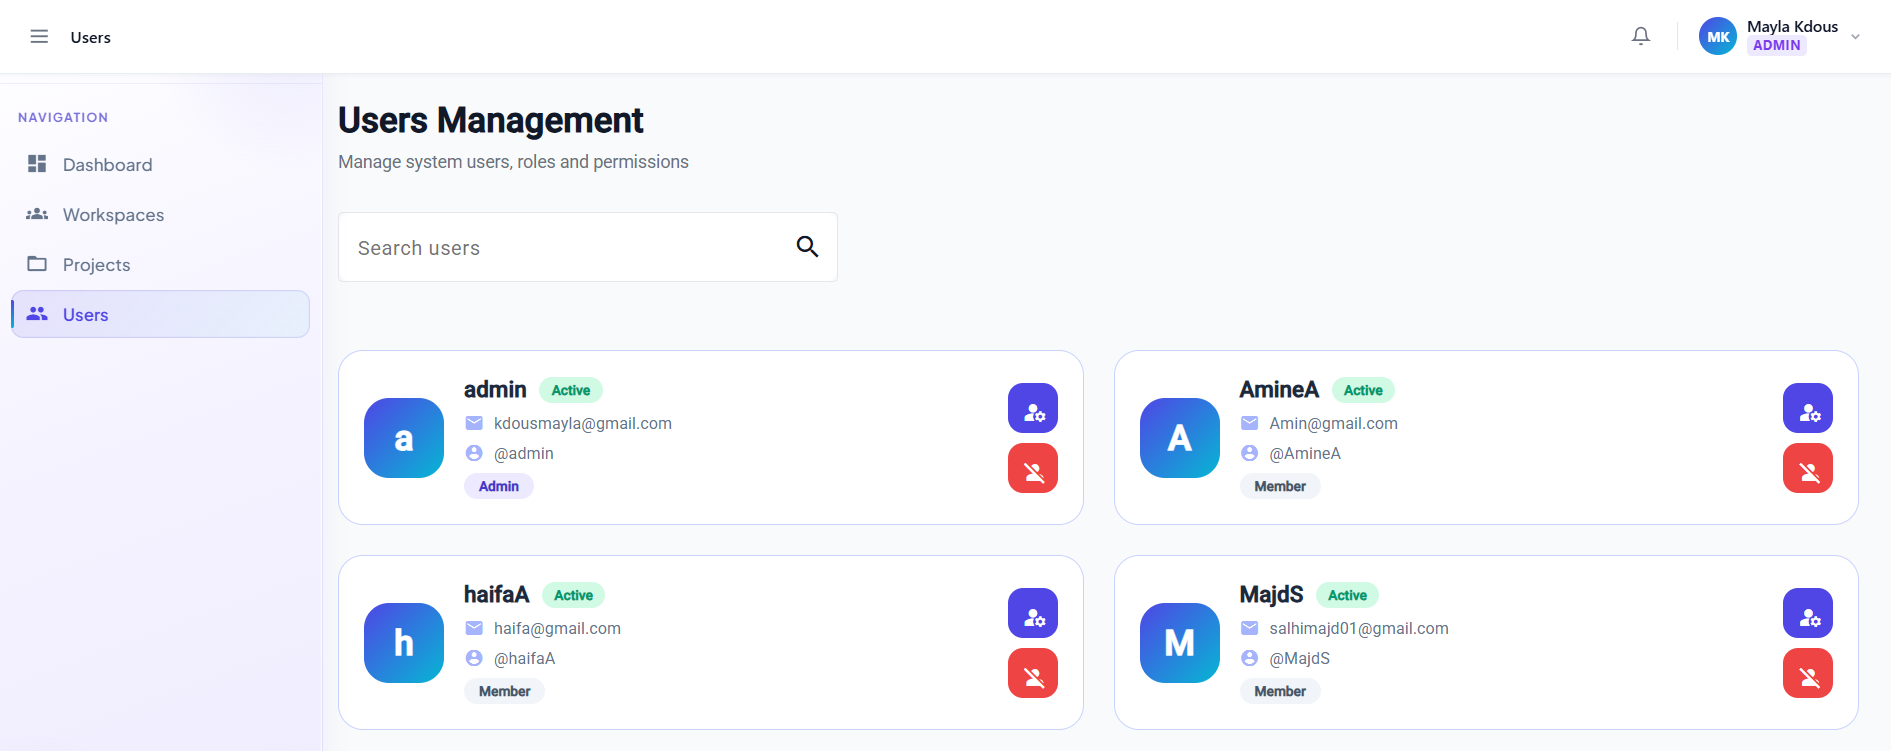
\includegraphics[width=0.9\columnwidth]{i3.png}
  \caption{Sprint 1 - Interface de gestion des utilisateurs}
  \label{fig:sprint1-users}
\end{figure}

La figure \ref{fig:sprint1-workspaces} illustre l'interface de consultation des espaces de travail accessibles à l'utilisateur.

\begin{figure}[H]
  \centering
  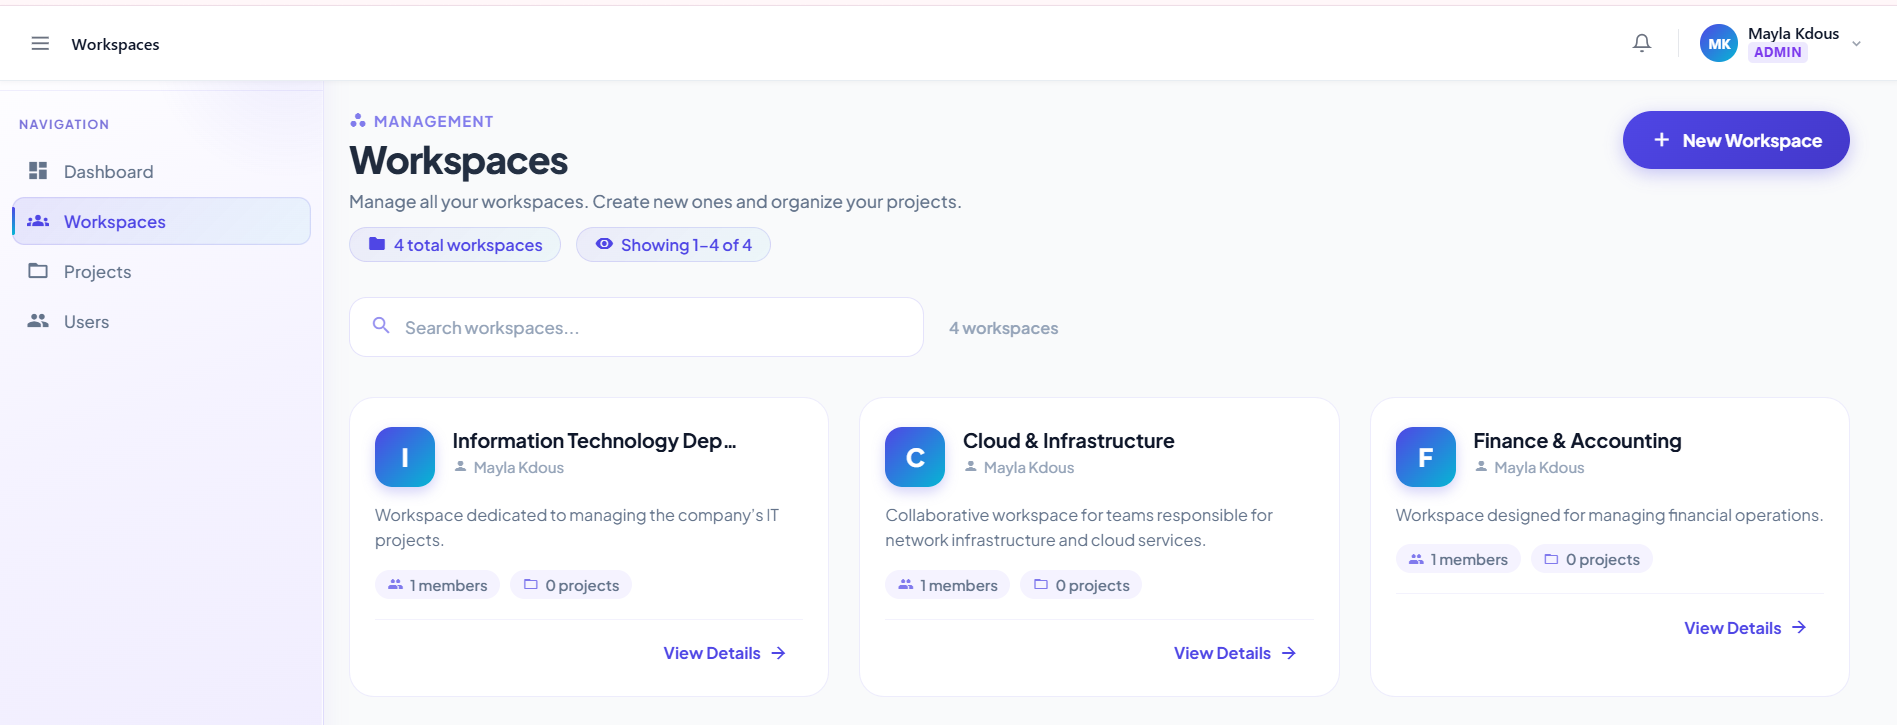
\includegraphics[width=0.9\columnwidth]{i4.png}
  \caption{Sprint 1 - Interface des espaces de travail}
  \label{fig:sprint1-workspaces}
\end{figure}

La figure \ref{fig:sprint1-projects} présente l'interface de gestion des projets.

\begin{figure}[H]
  \centering
  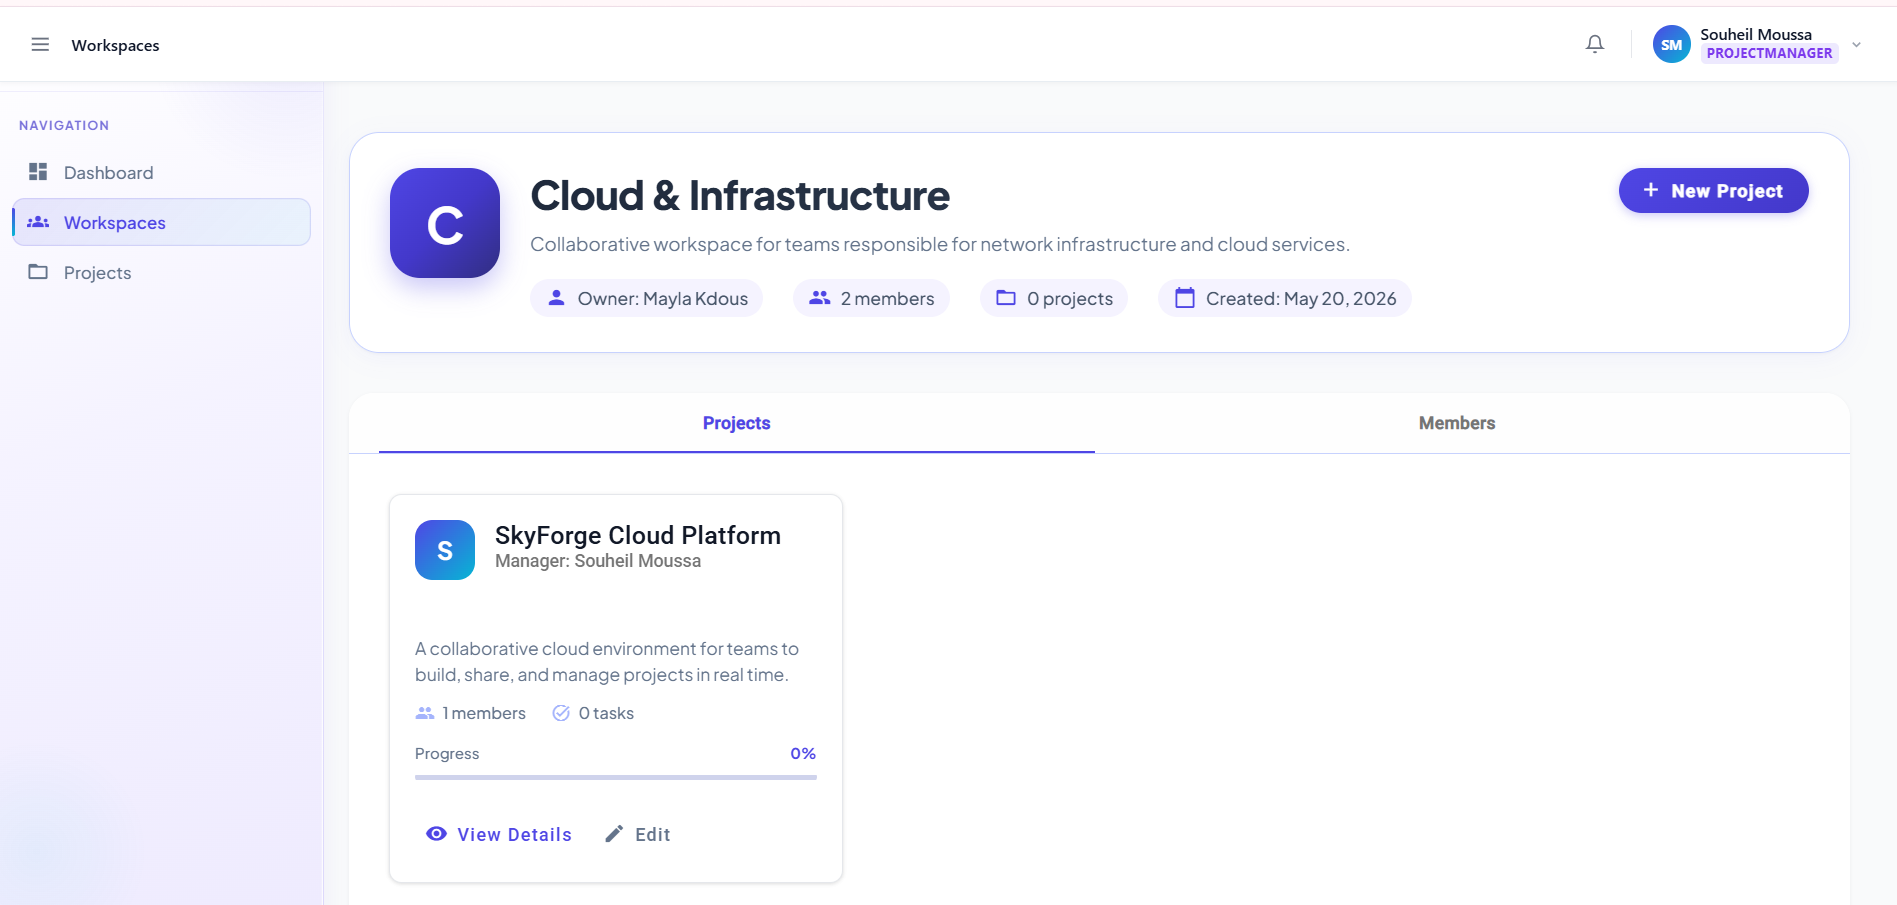
\includegraphics[width=0.9\columnwidth]{i5.png}
  \caption{Sprint 1 - Interface de gestion des projets}
  \label{fig:sprint1-projects}
\end{figure}

%------------------------------------------------------------
\subsection{Sprint 2 - Gestion agile : backlog, tâches, sprints et tableau de bord}
%------------------------------------------------------------
\subsubsection{Backlog du sprint}
Le tableau \ref{tab:backlog-sprint2} illustre le backlog du Sprint 2.

\begin{longtable}{|p{5.8cm}|p{1.3cm}|p{7.2cm}|}
  \caption{Backlog du Sprint 2 : Gestion agile, tâches, sprints et tableau de bord}\label{tab:backlog-sprint2} \\
  \hline
  \textbf{User Story} & \textbf{ID} & \textbf{Tâches} \\
  \hline
  \endfirsthead
  \hline
  \textbf{User Story} & \textbf{ID} & \textbf{Tâches} \\
  \hline
  \endhead
  \hline
  \endfoot
  \hline
  \endlastfoot

  \multirow{4}{*}{\begin{minipage}[t]{5.8cm}En tant que ProjectManager, je veux gérer le backlog afin d'organiser les besoins du projet.\end{minipage}}
                      & 2.1         & \textbullet~Créer l'entité BacklogItem et ses relations. \\
  \cline{2-3}
                      & 2.2         & \textbullet~Développer les opérations de création, modification et suppression des éléments du backlog. \\
  \cline{2-3}
                      & 2.3         & \textbullet~Ajouter la priorité, la complexité, les story points et la date d'échéance. \\
  \cline{2-3}
                      & 2.4         & \textbullet~Permettre l'affectation des éléments du backlog aux membres. \\
  \hline

  \multirow{3}{*}{\begin{minipage}[t]{5.8cm}En tant que membre, je veux suivre mes tâches afin de connaître mon travail à réaliser.\end{minipage}}
                      & 2.5         & \textbullet~Créer la gestion des tâches et des sous-tâches. \\
  \cline{2-3}
                      & 2.6         & \textbullet~Permettre la mise à jour de l'état et du pourcentage d'avancement. \\
  \cline{2-3}
                      & 2.7         & \textbullet~Ajouter les commentaires liés aux tâches et au backlog. \\
  \hline

  \multirow{3}{*}{\begin{minipage}[t]{5.8cm}En tant que ProjectManager, je veux gérer les sprints afin de planifier le travail par itérations.\end{minipage}}
                      & 2.8         & \textbullet~Créer l'entité Sprint et ses relations avec Project et TaskItem. \\
  \cline{2-3}
                      & 2.9         & \textbullet~Développer la création et la consultation des sprints. \\
  \cline{2-3}
                      & 2.10        & \textbullet~Créer le tableau de sprint pour suivre l'avancement. \\
  \hline

  \multirow{2}{*}{\begin{minipage}[t]{5.8cm}En tant qu'utilisateur, je veux consulter un tableau de bord afin de suivre l'avancement global.\end{minipage}}
                      & 2.11        & \textbullet~Calculer les indicateurs d'avancement des projets et workspaces. \\
  \cline{2-3}
                      & 2.12        & \textbullet~Créer l'interface du tableau de bord. \\
  \hline
\end{longtable}

\subsubsection{Interfaces livrables}

La figure \ref{fig:sprint2-backlog} illustre l'interface de gestion du backlog.

\begin{figure}[H]
  \centering
  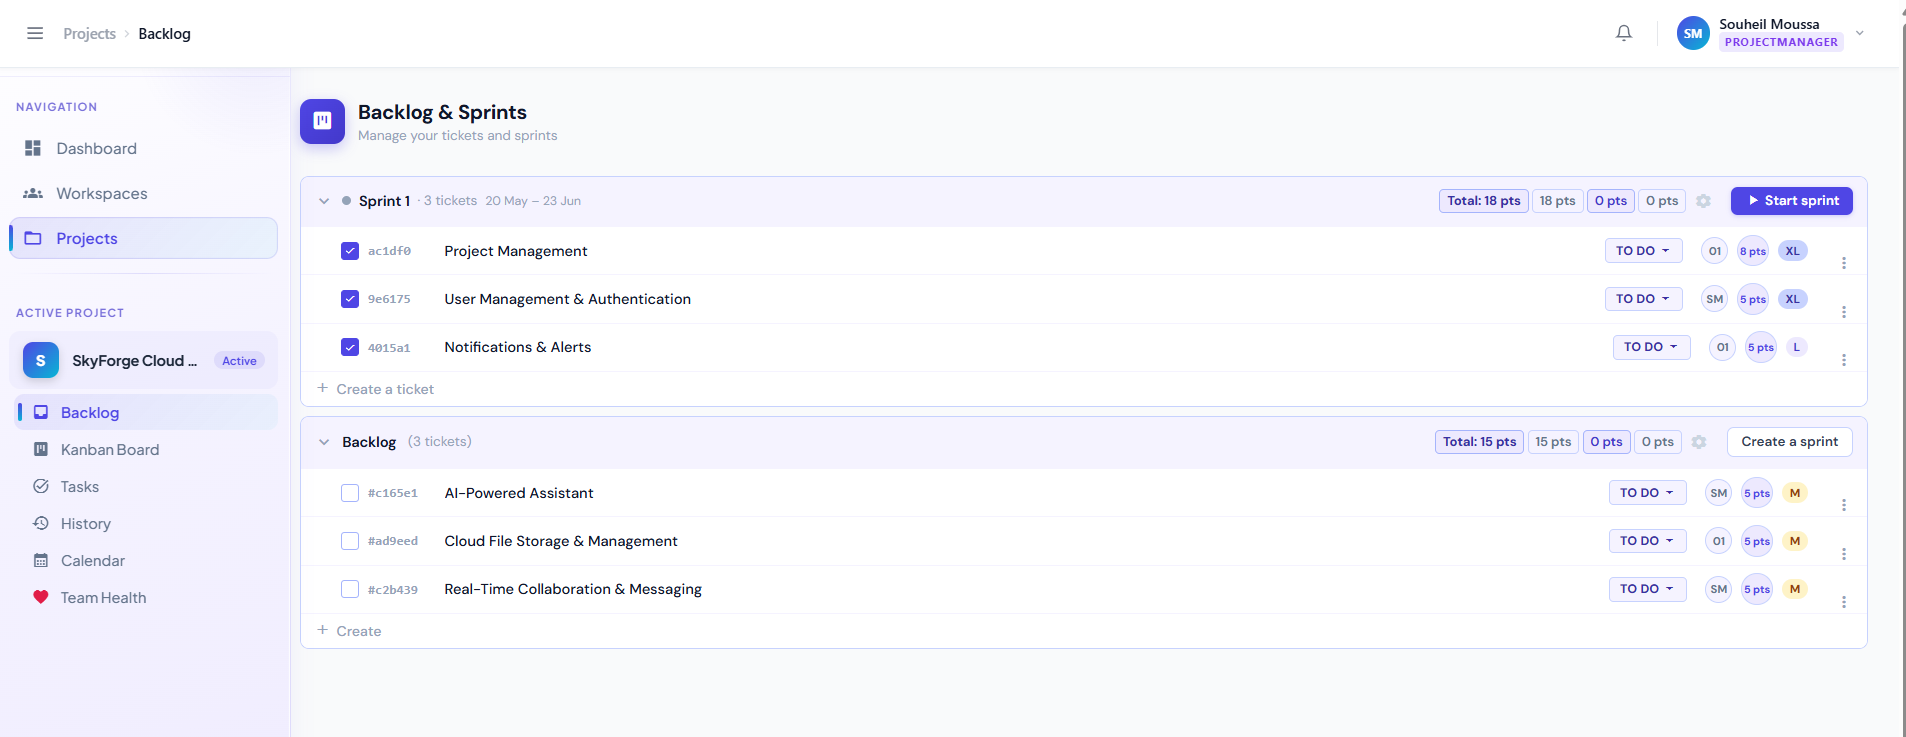
\includegraphics[width=0.9\columnwidth]{i6.png}
  \caption{Sprint 2 - Interface de gestion du backlog}
  \label{fig:sprint2-backlog}
\end{figure}

La figure \ref{fig:sprint2-board} présente le tableau agile permettant de suivre l'avancement des tâches du sprint.

\begin{figure}[H]
  \centering
  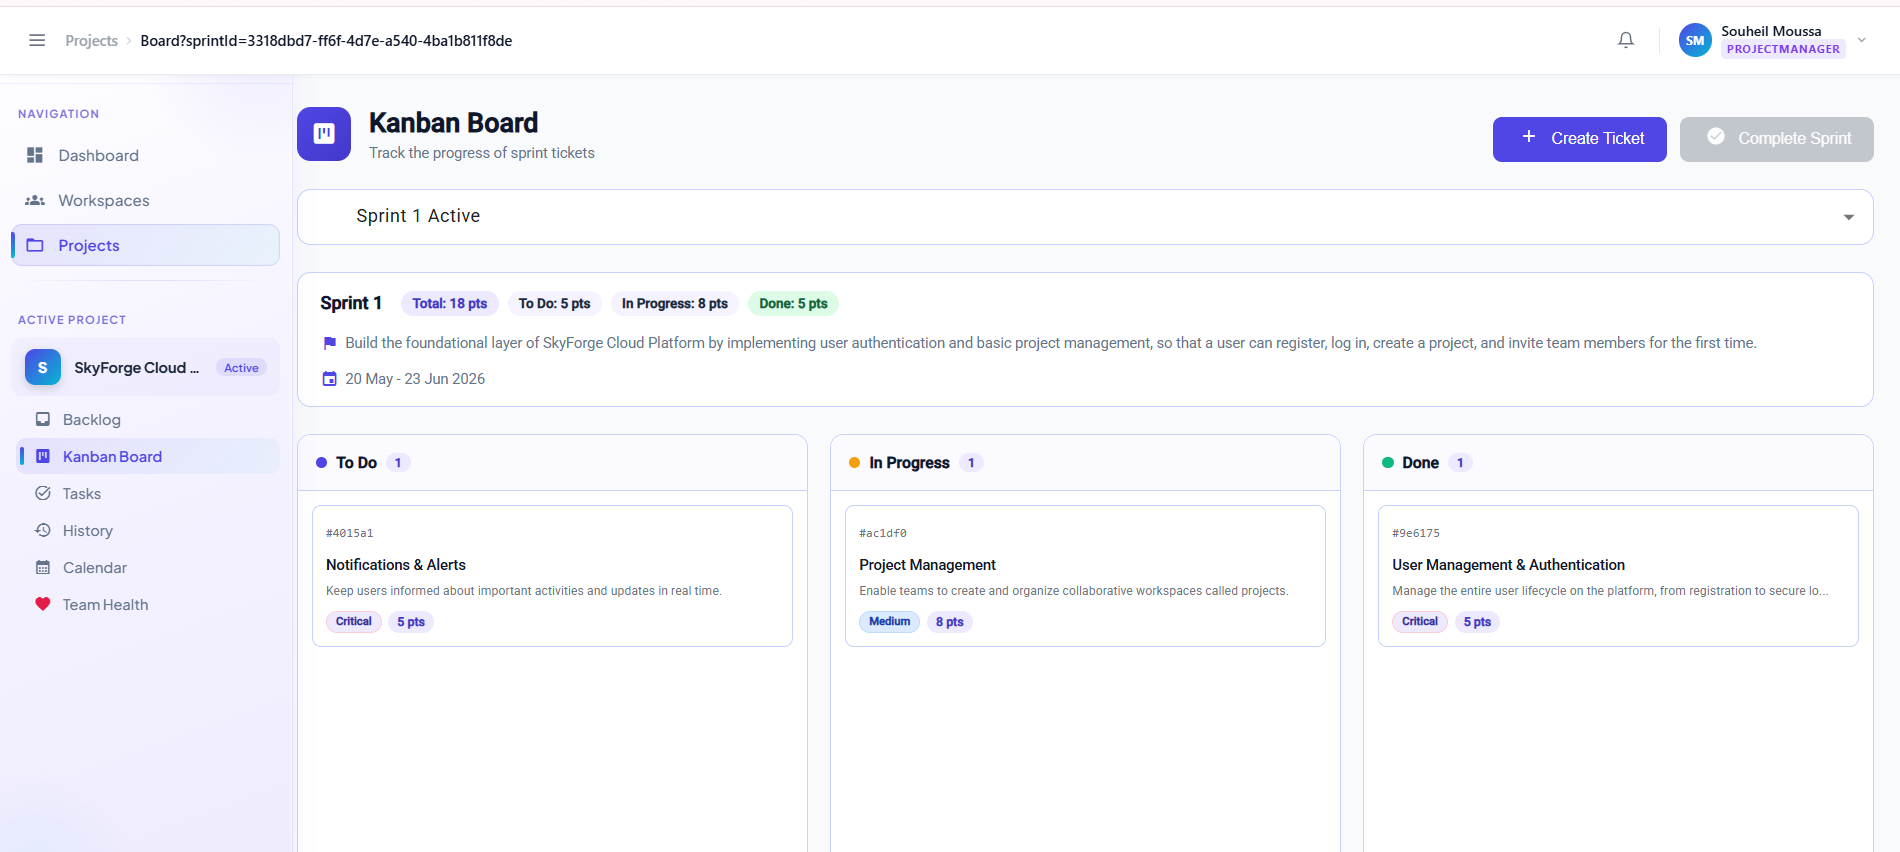
\includegraphics[width=0.9\columnwidth]{i7.png}
  \caption{Sprint 2 - Tableau de sprint}
  \label{fig:sprint2-board}
\end{figure}

La figure \ref{fig:sprint2-dashboard} illustre l'interface du tableau de bord.

\begin{figure}[H]
  \centering
  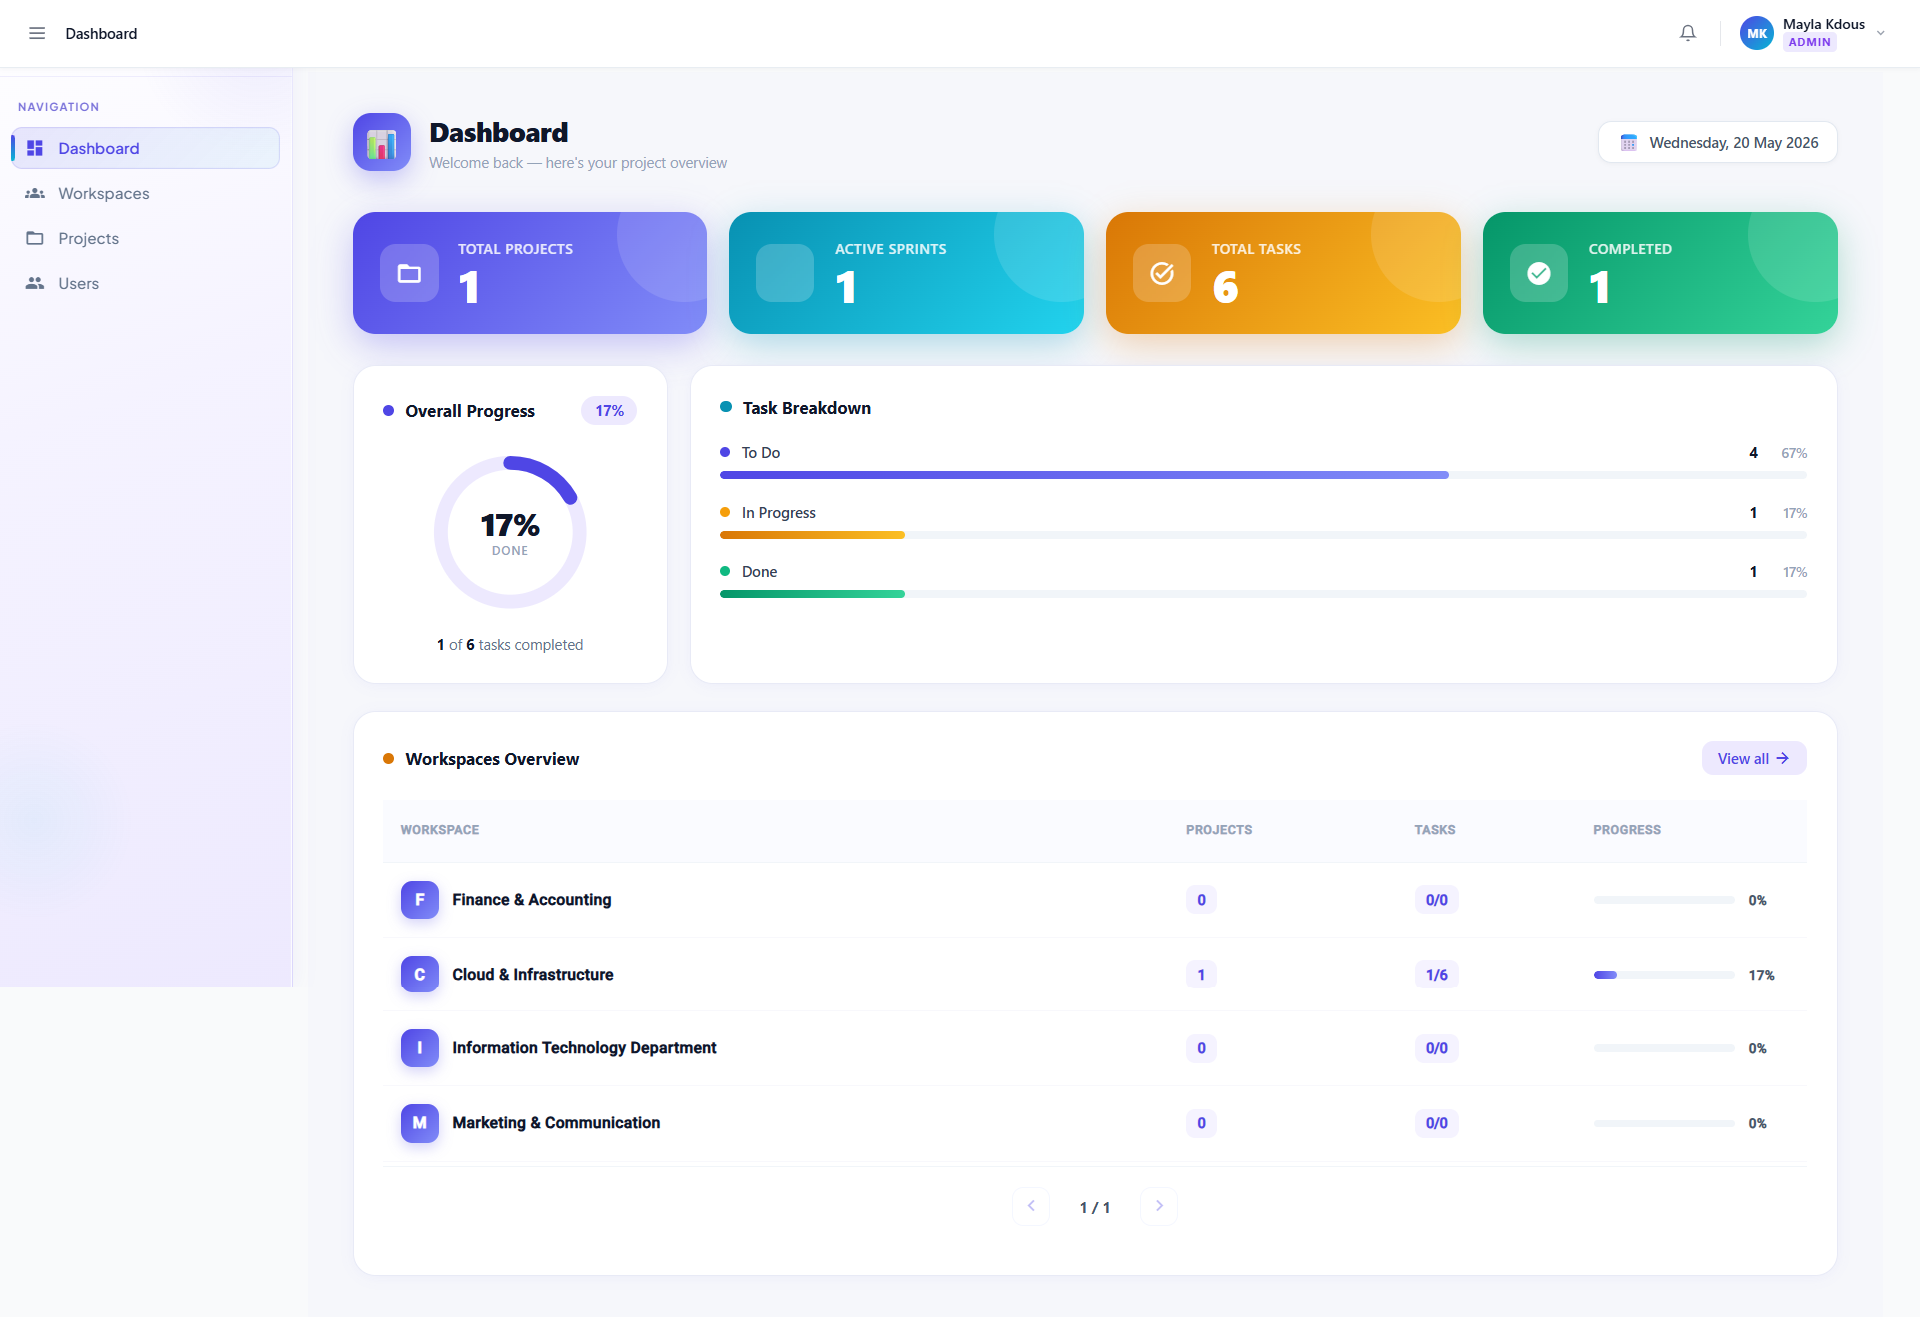
\includegraphics[width=0.7\columnwidth]{Planora.png}
  \caption{Sprint 2 - Interface de tableau de bord}
  \label{fig:sprint2-dashboard}
\end{figure}

%------------------------------------------------------------
\subsection{Sprint 3 - Collaboration, réunions et suivi de la santé de l'équipe par IA}
%------------------------------------------------------------
\subsubsection{Backlog du sprint}
Le tableau \ref{tab:backlog-sprint3} illustre le backlog du Sprint 3.

\begin{longtable}{|p{5.8cm}|p{1.3cm}|p{7.2cm}|}
  \caption{Backlog du Sprint 3 : Collaboration, réunions et suivi de la santé de l'équipe par IA}\label{tab:backlog-sprint3} \\
  \hline
  \textbf{User Story} & \textbf{ID} & \textbf{Tâches} \\
  \hline
  \endfirsthead
  \hline
  \textbf{User Story} & \textbf{ID} & \textbf{Tâches} \\
  \hline
  \endhead
  \hline
  \endfoot
  \hline
  \endlastfoot

  \multirow{3}{*}{\begin{minipage}[t]{5.8cm}En tant que membre de projet, je veux échanger avec mon équipe afin de faciliter la collaboration.\end{minipage}}
                      & 3.1         & \textbullet~Créer les entités ChatSession et ChatMessage. \\
  \cline{2-3}
                      & 3.2         & \textbullet~Développer l'espace de messagerie par projet. \\
  \cline{2-3}
                      & 3.3         & \textbullet~Ajouter les réactions, réponses et pièces jointes aux messages. \\
  \hline

  \multirow{3}{*}{\begin{minipage}[t]{5.8cm}En tant que membre de projet, je veux planifier des réunions afin d'organiser les échanges de l'équipe.\end{minipage}}
                      & 3.4         & \textbullet~Créer la gestion des événements de réunion. \\
  \cline{2-3}
                      & 3.5         & \textbullet~Afficher les réunions dans un calendrier. \\
  \cline{2-3}
                      & 3.6         & \textbullet~Permettre la sélection des membres concernés par une réunion. \\
  \hline

  \multirow{3}{*}{\begin{minipage}[t]{5.8cm}En tant que ProjectManager, je veux analyser les messages de l'équipe afin de détecter l'ambiance générale du projet.\end{minipage}}
                      & 3.7         & \textbullet~Préparer le modèle d'analyse des sentiments. \\
  \cline{2-3}
                      & 3.8         & \textbullet~Développer l'\ac{API} Flask d'analyse des messages. \\
  \cline{2-3}
                      & 3.9         & \textbullet~Connecter le module IA à la base de données et aux messages du projet. \\
  \hline

  \multirow{3}{*}{\begin{minipage}[t]{5.8cm}En tant que membre ou ProjectManager, je veux consulter les indicateurs de santé de l'équipe afin d'identifier les situations à risque.\end{minipage}}
                      & 3.10        & \textbullet~Classifier les messages en positif, neutre, stressé ou frustré. \\
  \cline{2-3}
                      & 3.11        & \textbullet~Calculer un score global de santé de l'équipe. \\
  \cline{2-3}
                      & 3.12        & \textbullet~Afficher la distribution des sentiments, les alertes et le résumé par membre. \\
  \hline
\end{longtable}

\subsubsection{Interfaces livrables}

La figure \ref{fig:sprint3-chat} illustre l'interface de messagerie du projet.

\begin{figure}[H]
  \centering
  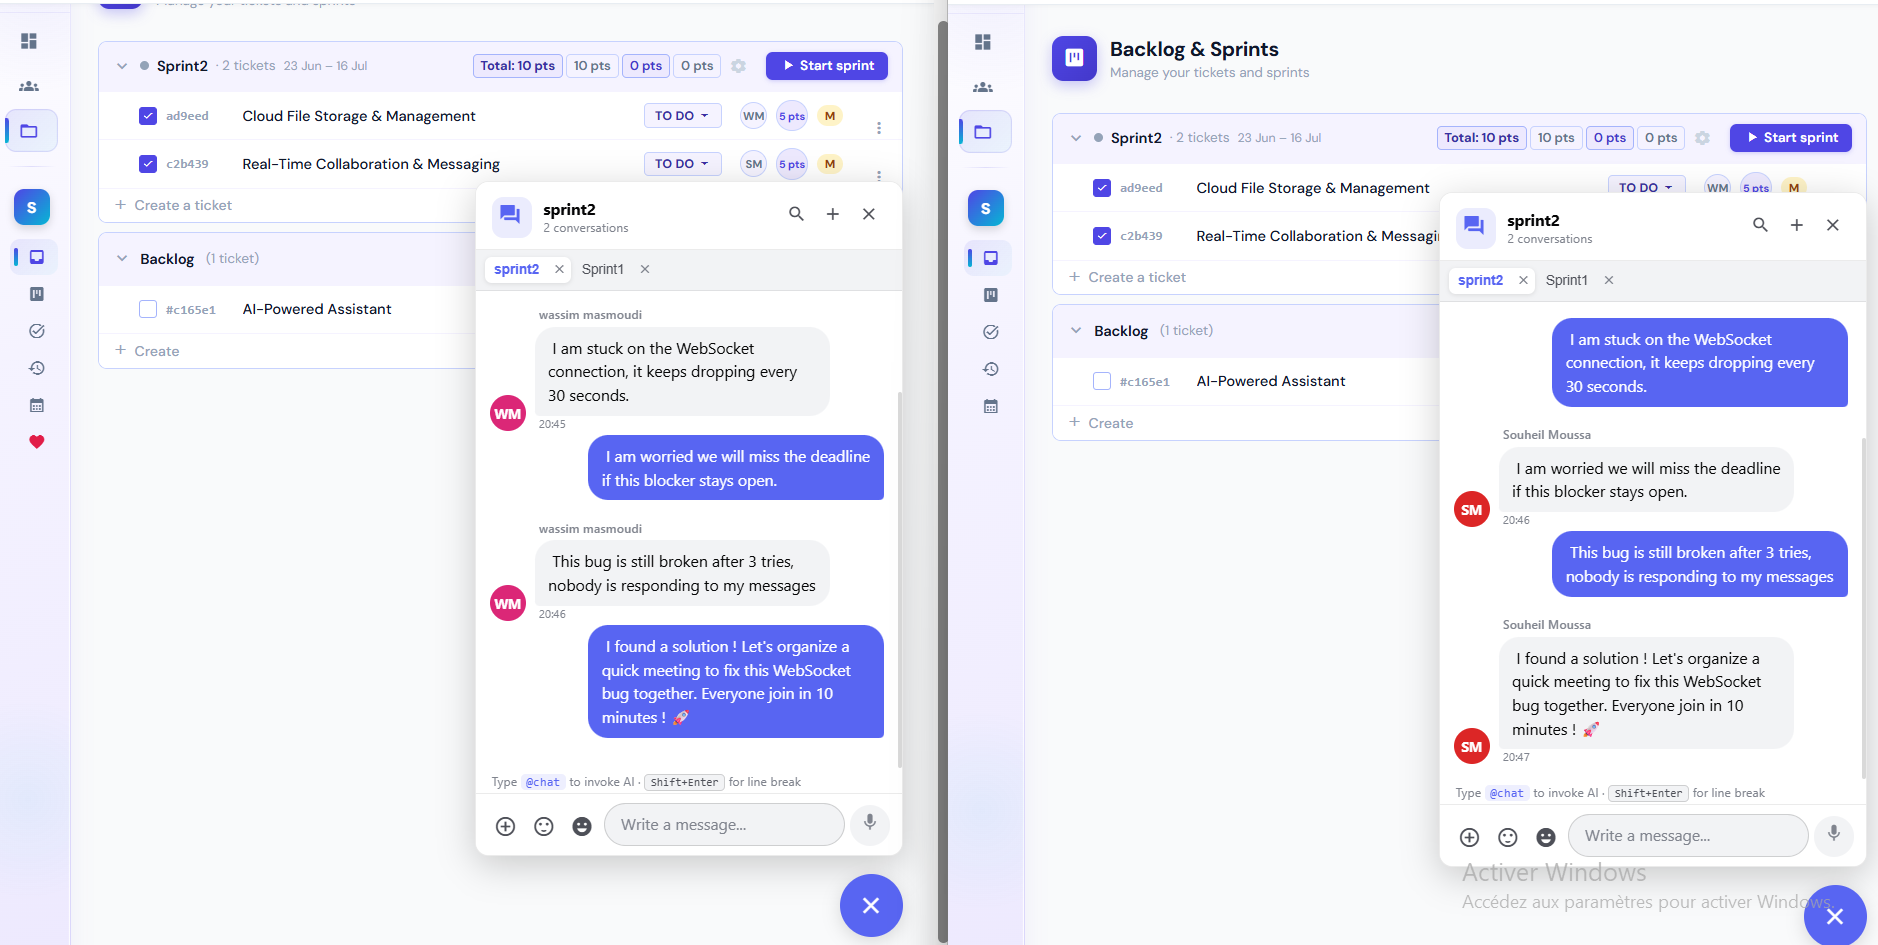
\includegraphics[width=0.9\columnwidth]{i8.png}
  \caption{Sprint 3 - Interface de messagerie}
  \label{fig:sprint3-chat}
\end{figure}

La figure \ref{fig:sprint3-calendar} présente le calendrier des réunions du projet.

\begin{figure}[H]
  \centering
  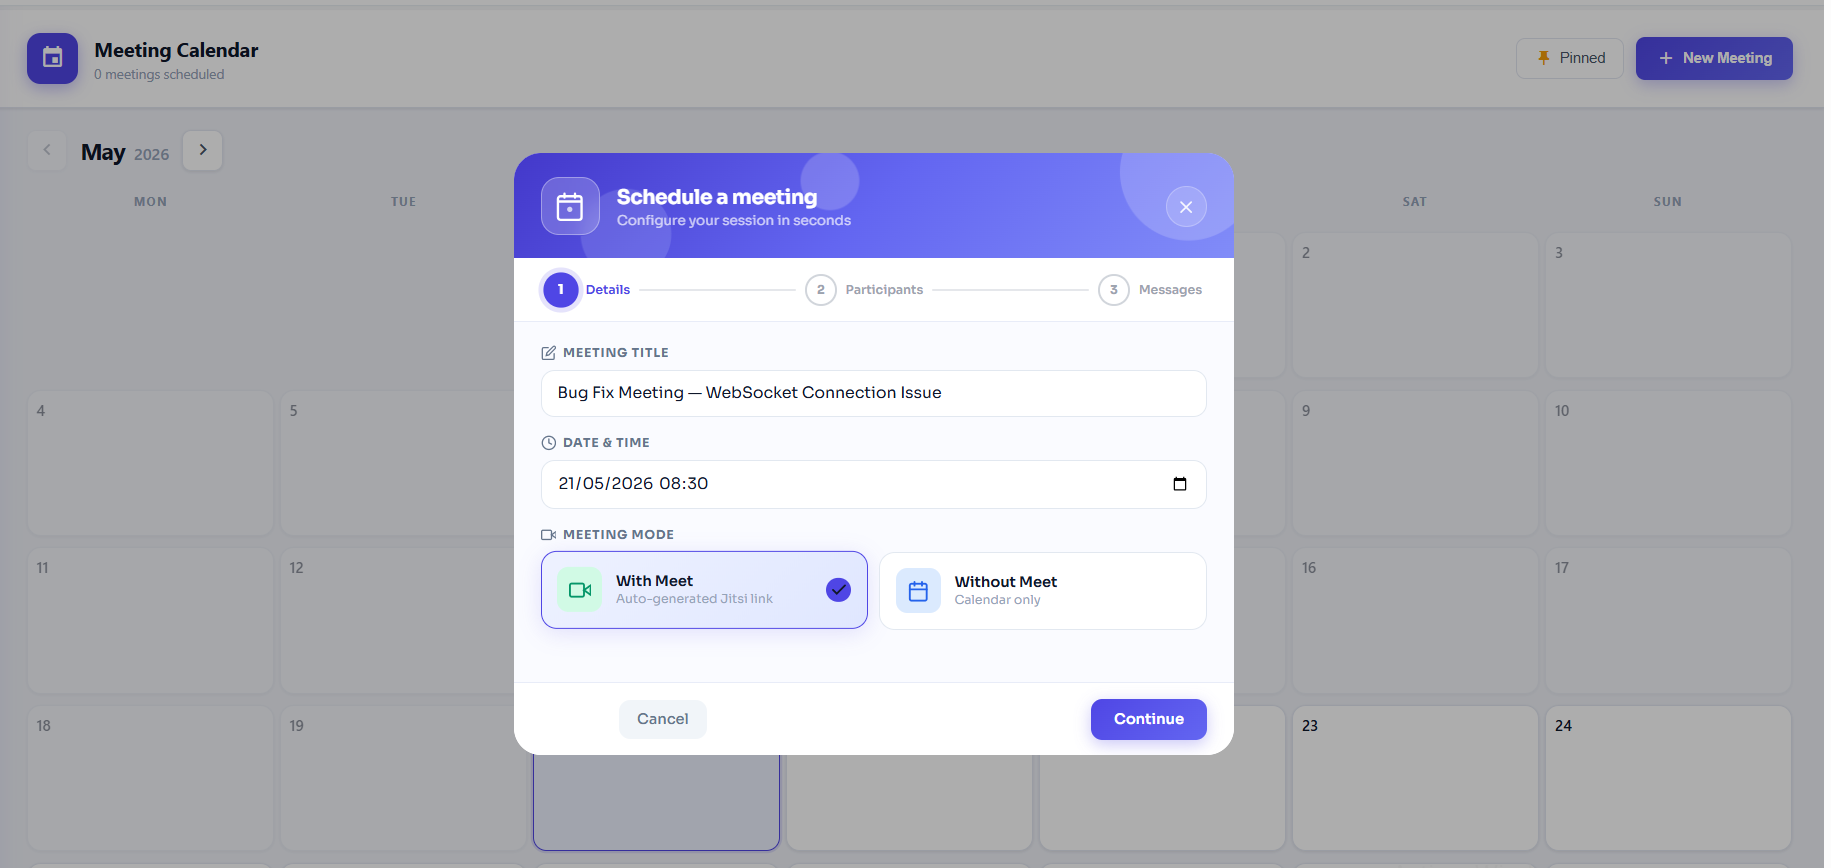
\includegraphics[width=0.9\columnwidth]{i9.png}
  \caption{Sprint 3 - Calendrier des réunions}
  \label{fig:sprint3-calendar}
\end{figure}

La figure \ref{fig:sprint3-teamhealth} illustre l'interface de suivi de la santé de l'équipe.

\begin{figure}[H]
  \centering
  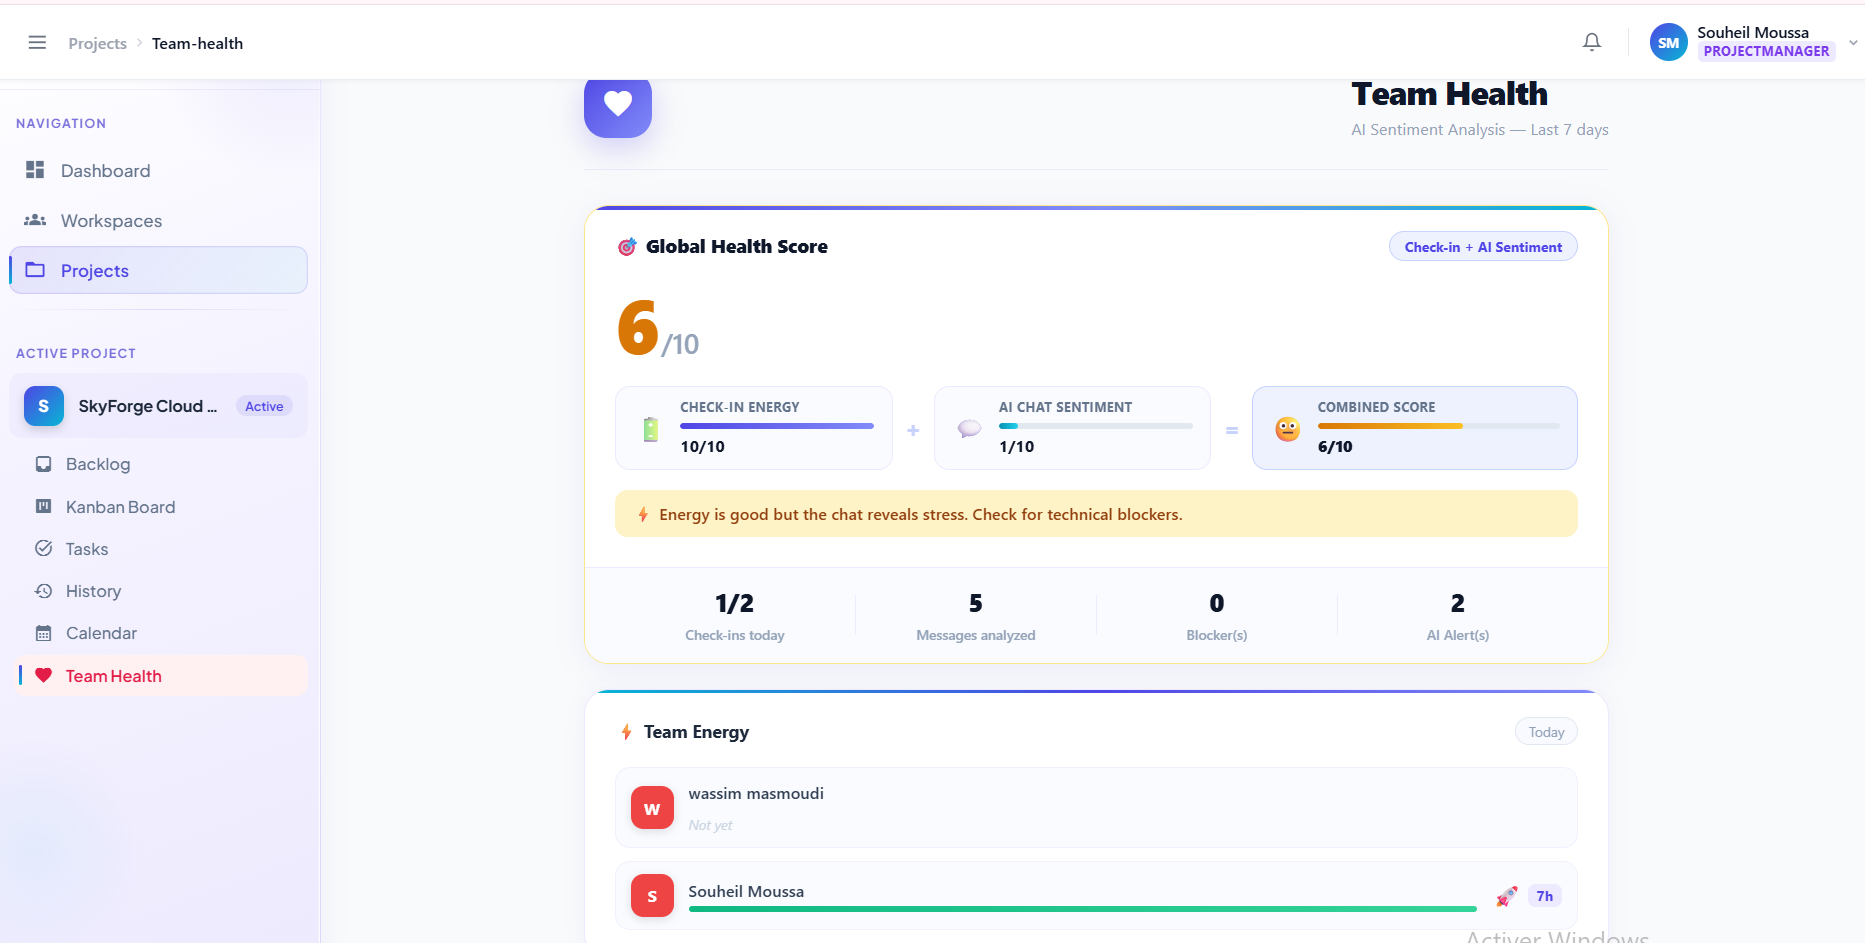
\includegraphics[width=0.7\columnwidth]{i10.png}
  \caption{Sprint 3 - Interface de suivi de la santé de l'équipe}
  \label{fig:sprint3-teamhealth}
\end{figure}

La figure \ref{fig:sprint3-ai-health} présente le résultat de test de l'API Flask dédiée à l'analyse des sentiments.

\begin{figure}[H]
  \centering
  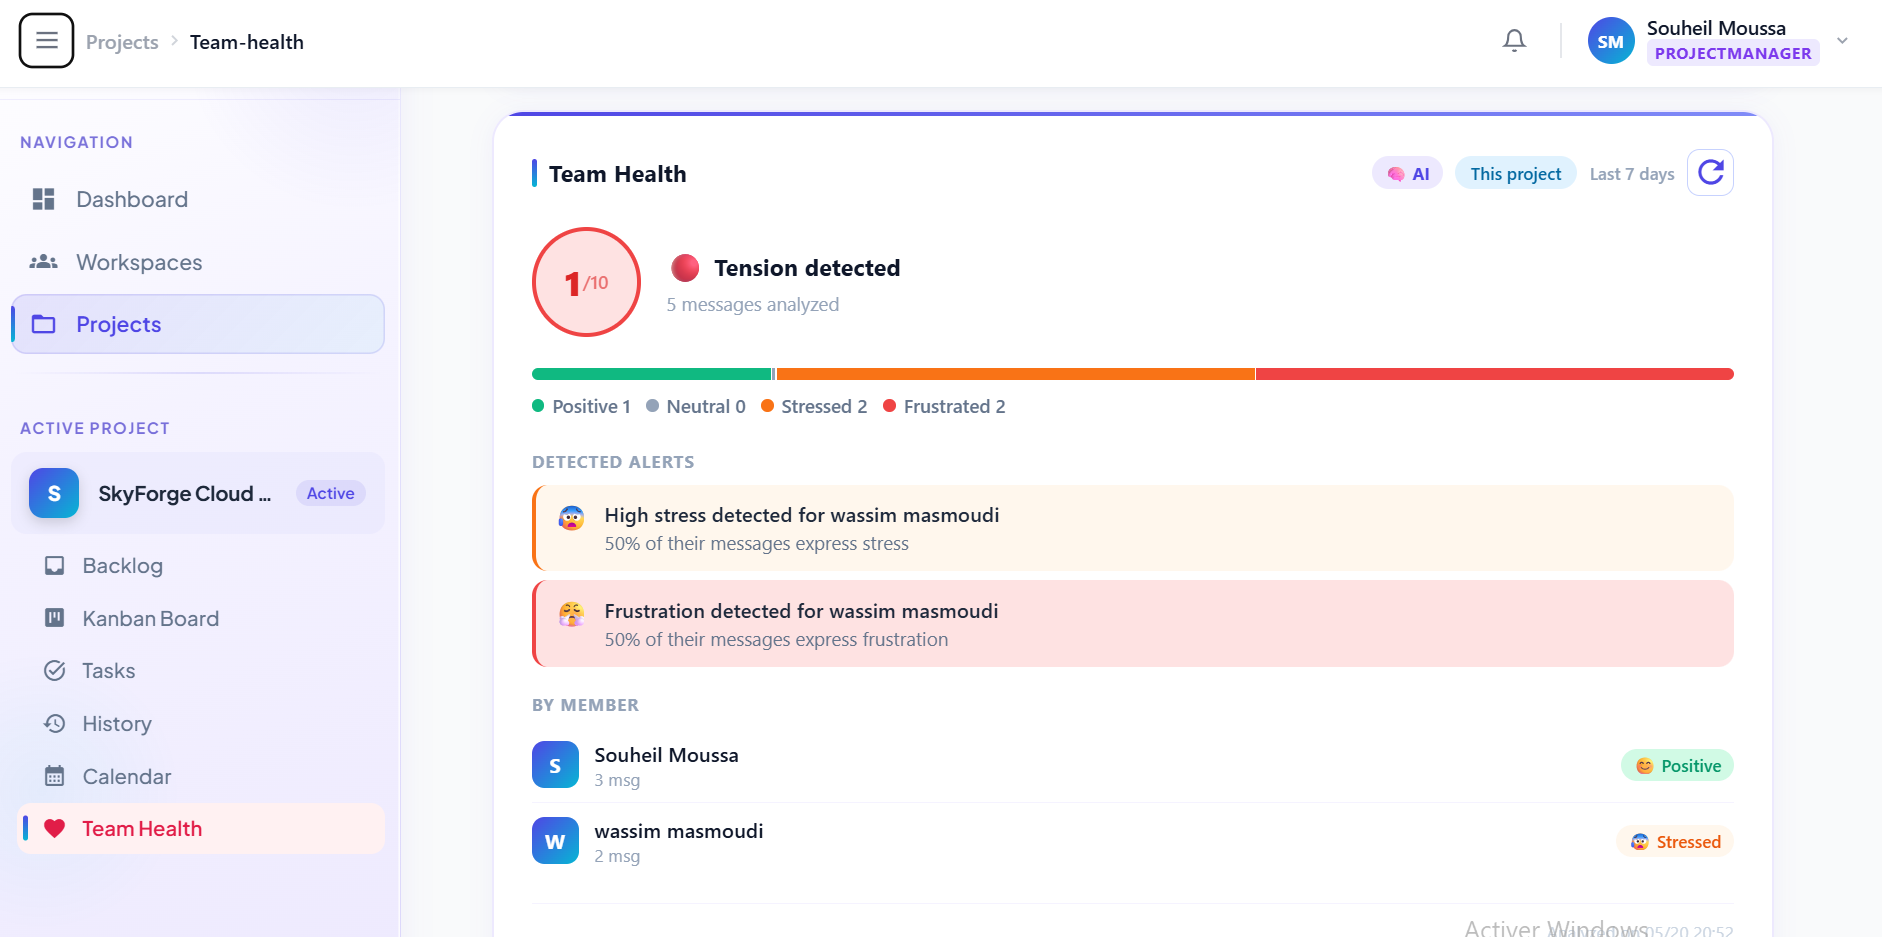
\includegraphics[width=0.7\columnwidth]{i11.png}
  \caption{Sprint 3 - Test du service IA d'analyse des sentiments}
  \label{fig:sprint3-ai-health}
\end{figure}

\section*{Conclusion}
Dans ce chapitre, nous avons présenté l'environnement logiciel, suivi de la mise en évidence de l'architecture technique des différentes couches de l'application. Enfin, nous avons détaillé les interfaces réalisées sprint par sprint, accompagnées des captures d'écran et des tests des services implémentés.

%\appendix
\chapter*{}
\vspace{-3em}
{\raggedleft\huge\bfseries Conclusion générale\par}
\vspace{2em}
\label{chap:concl}

Ce rapport présente le travail accompli dans le cadre de notre projet de développement portant sur la conception et le développement de l'application Planora. Il expose en détail les différentes étapes suivies pour analyser, concevoir et réaliser une plateforme web de gestion de projet, itération par itération, en suivant une méthodologie hybride.\\
Le champ d'application de Planora englobe plusieurs modules, notamment la gestion des utilisateurs et de leurs rôles, la gestion des espaces de travail, la création et le suivi des projets, la gestion du backlog, des tâches, des sous-tâches et des sprints, ainsi que la collaboration entre les membres à travers la messagerie et les réunions. L'application intègre également un module d'intelligence artificielle permettant d'analyser les messages échangés afin de suivre la santé de l'équipe et de détecter les signes de stress ou de frustration.\\
Au cours de la réalisation de ce projet, nous avons eu l'opportunité d'appliquer et de renforcer nos connaissances en développement web, en architecture logicielle, en conception UML, en gestion de projet agile et en intégration de services intelligents. Ce travail nous a également permis de mieux comprendre les besoins liés à la collaboration au sein des équipes projet et l'importance d'une solution centralisée pour améliorer l'organisation et le suivi.\\
En ce qui concerne les perspectives futures, plusieurs améliorations peuvent être envisagées, notamment l'enrichissement du module d'intelligence artificielle, l'ajout de notifications en temps réel plus avancées, l'intégration avec des outils externes tels que GitHub, Google Calendar ou Slack, ainsi que l'amélioration des tableaux de bord analytiques. Ces évolutions permettront de renforcer l'efficacité de Planora et d'offrir une expérience plus complète aux équipes de projet.

\backmatter
%%%%% Bibliography, in BibTeX format (the references.bib file)
\bibliography{references}

% \newgeometry{
bottom=18mm,
left=20mm,
top=18mm,
right=20mm
}

\thispagestyle{empty}

\begin{center}

\begin{minipage}{0.9\textwidth}

% ---------------- Arabic ----------------

\begin{Arabic}

{\Large\textbf{ملخّص}}

\vspace{4mm}

يوضع الملخص باللغة العربية هنا. يجب أن يقدّم هذا القسم وصفاً موجزاً
لموضوع المشروع، الأهداف الرئيسية، والمنهجية المتبعة والنتائج
المتحصل عليها. يُفضّل أن لا يتجاوز الملخص عشر أسطر.

\vspace{4mm}

\textbf{كلمات مفتاحيّة:} كلمة1، كلمة2، كلمة3، كلمة4، كلمة5

\end{Arabic}

\vspace{10mm}

% ---------------- French ----------------

\begin{french}

{\Large\textbf{Résumé}}

\vspace{4mm}

Mettez le résumé en français ici. Cette section doit présenter
brièvement le contexte du projet, les objectifs principaux,
la méthodologie utilisée ainsi que les résultats obtenus.
Merci de ne pas dépasser une dizaine de lignes.

\vspace{4mm}

\textbf{Mots clés :} mot1, mot2, mot3, mot4, mot5

\end{french}

\vspace{10mm}

% ---------------- English ----------------

{\Large\textbf{Abstract}}

\vspace{4mm}

Put the English abstract here. This section should briefly describe
the project context, the main objectives, the methodology used,
and the obtained results. Please do not exceed ten lines.

\vspace{4mm}

\textbf{Keywords:} keyword1, keyword2, keyword3, keyword4, keyword5

\end{minipage}

\end{center}

\restoregeometry

\end{document}
